%=====================================================================
% CUADERNO DE ALGORITMOS CUÁNTICOS
% Notas de estudio sobre el capítulo 6 (secciones 6.1-6.4) de
% N. S. Yanofsky y M. A. Mannucci, "Quantum Computing for Computer Scientists".
% Sigue la estructura de cuaderno_cuantica.tex. Pensado para imprimir a doble
% cara: capítulos y secciones empiezan en página derecha (impar), las páginas
% en blanco no llevan cabecera ni número, y las cajas no se parten entre páginas.
%
% Para compilar en Overleaf: subir este archivo y la carpeta figuras_yanofsky/.
%=====================================================================
\documentclass[11pt, a4paper, twoside, openright]{report}

% --- Idioma y codificación ---
\usepackage[utf8]{inputenc}
\usepackage[T1]{fontenc}
\usepackage[spanish, es-noshorthands, es-tabla]{babel}

% --- Márgenes: margen extra en el lado del lomo para encuadernar ---
\usepackage[a4paper, top=2.5cm, bottom=2.5cm, inner=3cm, outer=2cm, bindingoffset=0.5cm]{geometry}

% --- Matemáticas, figuras, color, código ---
\usepackage{amsmath, amssymb, amsthm}
\usepackage{graphicx}
\graphicspath{{figuras_yanofsky/}}
\usepackage{xcolor}
\usepackage{listings}
\usepackage[most]{tcolorbox}   % las cajas NO se parten entre páginas (no se usa breakable)
\usepackage{array}

% --- Circuitos cuánticos ---
\usepackage{tikz}
\usetikzlibrary{quantikz2}
\usetikzlibrary{arrows.meta, calc}

% --- Páginas en blanco sin cabecera ni número ---
\usepackage{emptypage}

% --- Colores: rosa claro y salmón ---
\definecolor{rosa}{RGB}{194,24,91}        % marcos de teoría
\definecolor{rosaclaro}{RGB}{248,187,208} % fondos de ejemplos
\definecolor{rosaviejo}{RGB}{199,94,128}  % marcos de ejemplos y ejercicios
\definecolor{salmon}{RGB}{233,114,76}     % aclaraciones y convenciones
\definecolor{tinta}{RGB}{51,51,51}

% --- Cabeceras: capítulo en páginas pares, sección en impares ---
\usepackage{fancyhdr}
\pagestyle{fancy}
\fancyhf{}
\fancyhead[LE]{\small\nouppercase{\leftmark}}
\fancyhead[RO]{\small\nouppercase{\rightmark}}
\fancyfoot[LE,RO]{\thepage}
\renewcommand{\headrulewidth}{0.4pt}
\renewcommand{\headrule}{\hbox to\headwidth{\color{rosa!60}\leaders\hrule height \headrulewidth\hfill}}
\setlength{\headheight}{14.5pt}
\setlength{\emergencystretch}{3em}  % evita líneas que se salen del margen

% --- Cajas (mismo código de colores en todo el documento) ---
\tcbset{enhanced, fonttitle=\bfseries, before skip=8pt, after skip=8pt}
\newtcolorbox{teoria}[1]{colback=rosa!5!white, colframe=rosa!85!black, title={#1}}
\newtcolorbox{demo}[1][Demostración]{colback=gray!5!white, colframe=gray!65!black, title={#1}}
\newtcolorbox{aclaracion}[1]{colback=salmon!7!white, colframe=salmon!85!black, title={#1}}
\newtcolorbox{ejemplo}[1]{colback=rosaclaro!18!white, colframe=rosaviejo, title={#1}}
\newtcolorbox{ejercicio}[1]{colback=white, colframe=rosaviejo, title={#1}, borderline={0.4pt}{2pt}{rosaviejo!40}}
\newtcolorbox{convencion}[1]{colback=salmon!14!white, colframe=salmon!70!black, title={Diferencia con Yanofsky: #1}}
\newtcolorbox{tfg}[1][Conexión con el TFG]{colback=rosa!9!white, colframe=rosa!55!black, title={#1}}
% Cajas de imágenes: fondo gris clarito y bordes rectos
\newtcolorbox{cajafigura}{colback=gray!10, colframe=gray!40, sharp corners, boxrule=0.4pt, halign=center}

% Paso del resumen guiado: cálculo arriba, concepto abajo
\newcommand{\pasoguiado}[3]{%
\begin{tcolorbox}[colback=gray!6!white,colframe=gray!55!black,title={#1}]
#2
\tcblower
\small #3
\end{tcolorbox}}

% --- Notación ---
\providecommand{\ket}[1]{|#1\rangle}
\providecommand{\bra}[1]{\langle #1|}
\providecommand{\braket}[2]{\langle #1|#2\rangle}
\newcommand{\bx}{\mathbf{x}}
\newcommand{\by}{\mathbf{y}}
\newcommand{\bz}{\mathbf{z}}
\newcommand{\bc}{\mathbf{c}}
\newcommand{\bw}{\mathbf{w}}
\newcommand{\bcero}{\mathbf{0}}
\newcommand{\bits}[1]{\{0,1\}^{#1}}
\newcommand{\F}{\mathbb{F}_2}
\newcommand{\Yan}[1]{\textcolor{rosaviejo}{\small[Y~#1]}}  % referencia a una ecuación del libro

% --- Configuración del código Python ---
\lstset{
    language=Python,
    basicstyle=\small\ttfamily,
    backgroundcolor=\color{gray!10},
    frame=single,
    rulecolor=\color{black!30},
    keywordstyle=\color{rosa}\bfseries,
    commentstyle=\color{gray!70!black}\itshape,
    stringstyle=\color{salmon!80!black},
    showstringspaces=false,
    breaklines=true,
    inputencoding=utf8,
    extendedchars=true,
    literate={á}{{\'a}}1 {é}{{\'e}}1 {í}{{\'i}}1 {ó}{{\'o}}1 {ú}{{\'u}}1 {ñ}{{\~n}}1 {Á}{{\'A}}1 {É}{{\'E}}1 {Í}{{\'I}}1 {Ó}{{\'O}}1 {Ú}{{\'U}}1 {Ñ}{{\~N}}1 {¿}{{?`}}1 {⊗}{{$\otimes$}}1 {⟩}{{$\rangle$}}1 {√}{{$\surd$}}1 {·}{{$\cdot$}}1
}
% Bloque de código que no se parte entre páginas
\lstnewenvironment{codigo}[1][]{\lstset{#1}\endgraf\noindent\minipage{\linewidth}}{\endminipage\endgraf\medskip}

% --- Enlaces (se carga el último) ---
\usepackage{hyperref}
\hypersetup{colorlinks=true, linkcolor=rosa!80!black, urlcolor=salmon!80!black, citecolor=rosaviejo,
            pdftitle={Cuaderno de Algoritmos Cuánticos}}

\begin{document}

% =========================== PORTADA ================================
\begin{titlepage}
\centering
\vspace*{4cm}
{\Huge\bfseries Cuaderno de Algoritmos Cuánticos\par}
\vspace{1cm}
{\Large Deutsch, Deutsch--Jozsa, Simon y Grover\par}
\vspace{1cm}
{\color{rosa!60}\rule{0.5\textwidth}{1pt}\par}
\vspace{1cm}
{\large Notas de estudio sobre el capítulo 6 (secciones 6.1--6.4) de\\[2mm] N.~S.~Yanofsky y M.~A.~Mannucci, \textit{Quantum Computing for Computer Scientists}\par}
\vfill
{\large Elia Torres Simón\par}
\vspace{0.5cm}
{\large Trabajo de Fin de Grado --- Grado en Matemáticas, UCM\par}
\vspace{0.5cm}
{\large \today\par}
\end{titlepage}

% ========================== PRESENTACIÓN ============================
\cleardoublepage
\thispagestyle{empty}
\section*{Sobre este cuaderno}

\noindent Este cuaderno desarrolla la lectura asignada para la próxima reunión: las secciones 6.1 a 6.4 del capítulo 6 (\textit{Algorithms}) de Yanofsky y Mannucci \cite{yanofsky2008}. \textbf{La sección 6.5, el algoritmo de factorización de Shor, queda fuera.} Cada algoritmo se explica con todos los pasos intermedios, se demuestran los resultados que el libro solo enuncia (por ejemplo, el número de iteraciones de Grover, que el libro declara ``fuera del alcance del texto''), se resuelven los ejercicios del libro y se comprueba todo numéricamente en Qiskit.

\noindent Cada capítulo tiene la misma estructura que el \textit{Cuaderno de Computación Cuántica}:
\begin{itemize}
    \item \textbf{El problema y la solución clásica}, que hace de punto de referencia (el papel que allí tenía la ``información clásica'').
    \item \textbf{El algoritmo cuántico}, con la teoría completa, las demostraciones y los ejercicios resueltos.
    \item \textbf{Implementación en Qiskit}, donde se comprueban numéricamente los resultados.
    \item \textbf{Resumen: un ejemplo guiado}, que recorre todos los conceptos con un solo ejemplo y números concretos.
\end{itemize}

\begin{center}
\small\renewcommand{\arraystretch}{1.2}
\begin{tabular}{l|l|l}
\textbf{Capítulo} & \textbf{Yanofsky} & \textbf{Páginas del libro} \\ \hline
1. El algoritmo de Deutsch & Sección 6.1 & 170--179 \\
2. El algoritmo de Deutsch--Jozsa & Sección 6.2 & 179--187 \\
3. El algoritmo de periodicidad de Simon & Sección 6.3 & 187--195 \\
4. El algoritmo de búsqueda de Grover & Sección 6.4 & 195--204 \\
\textit{(excluido)} El algoritmo de Shor & Sección 6.5 & 204--219
\end{tabular}
\end{center}

\noindent Las referencias del tipo \Yan{6.27} remiten a la ecuación (6.27) del libro, para poder leer los dos textos en paralelo. Los ejercicios del libro aparecen resueltos con su numeración original (\textit{Ejercicio 6.1.3}, etc.).

\noindent \textbf{Código de colores de las cajas:}
\begin{itemize}
    \item \colorbox{rosa!5}{Rosa}: definiciones, proposiciones y teoremas.
    \item \colorbox{gray!8}{Gris}: demostraciones y pasos de los ejemplos guiados.
    \item \colorbox{salmon!10}{Salmón}: notas aclaratorias e intuición.
    \item \colorbox{salmon!18}{Salmón intenso}: \textbf{diferencias de convención con Yanofsky} (léelas antes de comparar una fórmula con el libro).
    \item \colorbox{rosaclaro!25}{Rosa claro}: ejemplos con números y ejercicios resueltos del libro.
\end{itemize}
Las cajas de \textbf{Conexión con el TFG} señalan las ideas que reaparecerán en los kernels cuánticos.

\noindent El código completo está en \texttt{algoritmos\_yanofsky.py}, ejecutado con Qiskit \textbf{versión 2.2.3}; las figuras están en la carpeta \texttt{figuras\_yanofsky}.

% ============================ ÍNDICE ================================
\cleardoublepage
\tableofcontents

% ===================== CONVENCIONES ==================================
\cleardoublepage
\chapter*{Antes de empezar: convenciones}
\addcontentsline{toc}{chapter}{Antes de empezar: convenciones}
\markboth{Antes de empezar: convenciones}{Antes de empezar: convenciones}

\noindent Yanofsky y Mannucci escriben los estados de varios qubits con una convención distinta de la de Qiskit (y de la del \textit{Cuaderno de Computación Cuántica}). La diferencia no cambia ningún resultado físico, pero sí cambia el aspecto de las matrices y el orden de los factores en los productos tensoriales. Este cuaderno usa \textbf{siempre la convención de Qiskit}; aquí se explica la traducción una sola vez, y en cada capítulo una caja salmón recuerda dónde aparece.

\subsection*{El orden de los qubits}

\begin{teoria}{Convención de este cuaderno (la de Qiskit)}
El cable \textbf{de arriba} del circuito es el qubit $\mathsf{q}_0$ y corresponde al factor \textbf{de la derecha} del producto tensorial y al último carácter de las cadenas de bits. Con $n$ qubits,
\[ \ket{b_{n-1}\cdots b_1 b_0} = \ket{b_{n-1}}\otimes\cdots\otimes\ket{b_1}\otimes\ket{b_0}, \qquad b_0 = \text{valor de } \mathsf{q}_0 \text{ (cable de arriba)}. \]
\textbf{Leer los cables de abajo arriba equivale a leer el ket de izquierda a derecha.}
\end{teoria}

\noindent Yanofsky hace lo contrario: en sus circuitos el cable de arriba es el factor de la \textbf{izquierda}. Por ejemplo, en el algoritmo de Deutsch el cable de arriba lleva el qubit de consulta $x$ y el de abajo el qubit de salida $y$, y el libro escribe el estado conjunto como $\ket{x,y} = \ket{x}\otimes\ket{y}$.

\noindent En este cuaderno \textbf{los circuitos se dibujan igual que en el libro} (consulta arriba, salida abajo), que es además como los dibuja Qiskit, pero los estados se escriben en el orden de Qiskit:
\[ \underbrace{\ket{x,y}}_{\text{Yanofsky}} \quad\longleftrightarrow\quad \underbrace{\ket{y}\ket{x} = \ket{y}\otimes\ket{x}}_{\text{este cuaderno}}. \]

\begin{center}
\small\renewcommand{\arraystretch}{1.35}
\begin{tabular}{l|l|l}
\textbf{Objeto} & \textbf{Yanofsky} & \textbf{Este cuaderno (Qiskit)} \\ \hline
Estado de entrada de Deutsch & $\ket{0,1} = \ket{0}\otimes\ket{1}$ & $\ket{1}\ket{0} = \ket{10}$ \\
Oráculo & $U_f\ket{x,y} = \ket{x,\,y\oplus f(x)}$ & $U_f\ket{y}\ket{x} = \ket{y\oplus f(x)}\ket{x}$ \\
Hadamard solo en el cable de arriba & $H\otimes I$ & $I\otimes H$ \\
Hadamard solo en el cable de abajo & $I\otimes H$ & $H\otimes I$ \\
Algoritmo de Deutsch completo & $(H\otimes I)\,U_f\,(H\otimes H)\ket{0,1}$ & $(I\otimes H)\,U_f\,(H\otimes H)\ket{1}\ket{0}$ \\
Índice de una entrada de $U_f$ & fila/columna $xy$ & fila/columna $yx$
\end{tabular}
\end{center}

\begin{teoria}{Proposición: las dos matrices de $U_f$ son conjugadas por el SWAP}
Sea $U^{\mathrm{Y}}$ la matriz de un operador de dos qubits escrita en el orden de Yanofsky (índices $xy$) y $U^{\mathrm{Q}}$ la del mismo operador en el orden de Qiskit (índices $yx$). Entonces
\[ U^{\mathrm{Q}} = \mathrm{SWAP}\; U^{\mathrm{Y}}\; \mathrm{SWAP}, \qquad \mathrm{SWAP}\,(\ket{a}\otimes\ket{b}) = \ket{b}\otimes\ket{a}. \]
En particular, $U^{\mathrm{Q}}$ y $U^{\mathrm{Y}}$ tienen los mismos autovalores, la misma traza y son unitarias a la vez: son \textbf{la misma operación escrita en otra base ordenada}.
\end{teoria}

\begin{demo}
Las dos matrices representan la misma aplicación lineal; solo cambia el orden en que se listan los vectores de la base. La entrada de $U^{\mathrm{Y}}$ en la fila $x'y'$ y la columna $xy$ es el coeficiente de $\ket{x'}\otimes\ket{y'}$ en la imagen de $\ket{x}\otimes\ket{y}$; la entrada de $U^{\mathrm{Q}}$ en la fila $y'x'$ y la columna $yx$ es el mismo número. Reordenar filas y columnas según la permutación $xy \mapsto yx$ es exactamente multiplicar a izquierda y derecha por la matriz de permutación de esa biyección, que es el SWAP (y $\mathrm{SWAP}^{-1} = \mathrm{SWAP}$). La conjugación por una matriz invertible conserva autovalores y traza, y la conjugación por una unitaria conserva la unitariedad. \hfill$\square$
\end{demo}

\begin{aclaracion}{Nota Aclaratoria: los nombres de los bits en las cadenas}
Yanofsky nombra los bits de una cadena de izquierda a derecha, $\bx = x_0x_1\cdots x_{n-1}$ (y en algún ejemplo $\bc = c_1c_2c_3$). En Qiskit el último carácter es $\mathsf{q}_0$. Para no arrastrar dos numeraciones, en este cuaderno \textbf{las cadenas se usan como etiquetas}: la función que el libro define sobre la cadena \texttt{10} se define aquí sobre la misma cadena \texttt{10}, leída al modo de Qiskit ($\mathsf{q}_1 = 1$, $\mathsf{q}_0 = 0$). Todas las cuentas del libro siguen valiendo tal cual, porque ningún algoritmo depende del nombre que se dé a cada posición: el producto binario $\bx\cdot\bz$ de la siguiente sección es simétrico respecto de cualquier reordenación aplicada a la vez a las dos cadenas. Cuando haga falta hablar de una posición concreta se dirá ``el primer bit por la izquierda''.
\end{aclaracion}

\subsection*{Producto interno y producto binario}

\noindent \textbf{Producto interno de estados.} Como en el cuaderno, $\braket{\psi}{\phi} = \sum_a \overline{\psi_a}\,\phi_a$ es \textbf{antilineal en el primer argumento}. Yanofsky usa la misma convención ($\langle V_1, V_2\rangle = V_1^\dagger V_2$, capítulo 2 del libro), así que aquí no hay que traducir nada.

\noindent \textbf{Producto binario de cadenas.} A partir de la sección 6.2, Yanofsky usa $\langle \bx,\by\rangle$ para algo distinto: la paridad del número de posiciones en que dos cadenas de bits valen $1$ a la vez. Para no confundirlo con el producto interno de estados, aquí se escribe con un punto:
\[ \bx\cdot\bz = x_{n-1}z_{n-1}\oplus\cdots\oplus x_1z_1\oplus x_0z_0 \in\{0,1\} \qquad \text{(Yanofsky: } \langle\bx,\bz\rangle\text{)}. \]
Por ejemplo, $\texttt{101}\cdot\texttt{111} = 1\oplus0\oplus1 = 0$ y $\texttt{110}\cdot\texttt{011} = 0\oplus1\oplus0 = 1$.

\subsection*{El esquema común de los algoritmos}

\noindent Yanofsky abre el capítulo con el esquema que siguen todos los algoritmos cuánticos que se van a estudiar \Yan{p.~171}:
\begin{enumerate}
    \item Los qubits empiezan en un \textbf{estado clásico} (un vector de la base estándar).
    \item Se ponen en una \textbf{superposición} de muchos estados (casi siempre con puertas de Hadamard).
    \item Se aplican \textbf{operaciones unitarias} a esa superposición, entre ellas la que evalúa la función.
    \item Se \textbf{miden} los qubits.
\end{enumerate}

\begin{teoria}{Definición: modelo de consultas}
En los cuatro problemas de este cuaderno se da una función $f$ como \textbf{caja negra} (un \textbf{oráculo}): se puede evaluar en las entradas que se quiera, pero no se puede ``mirar dentro'' para ver cómo está definida. El coste de un algoritmo se mide por el \textbf{número de consultas}, es decir, de evaluaciones de $f$. En el caso cuántico, una consulta es una aplicación de la puerta $U_f$, que se define en el Capítulo~1.
\end{teoria}

\noindent Esta forma de medir el coste es la que permite comparar con rigor: se cuentan consultas, no segundos, y se demuestra que ningún algoritmo clásico puede hacerlo con menos. Así se obtienen las ventajas de la tabla siguiente, que se irán demostrando capítulo a capítulo.

\begin{center}
\small\renewcommand{\arraystretch}{1.25}
\begin{tabular}{l|l|l|l}
\textbf{Problema} & \textbf{Clásico (determinista)} & \textbf{Cuántico} & \textbf{Ventaja} \\ \hline
Deutsch ($n=1$) & $2$ consultas & $1$ consulta & $2 \to 1$ \\
Deutsch--Jozsa & $2^{n-1}+1$ & $1$ & exponencial \\
Simon & $2^{n-1}+1$ & menos de $n+1$ ejecuciones en media & exponencial \\
Grover & $2^n$ (peor caso) & unas $\frac{\pi}{4}\sqrt{2^n}$ & cuadrática
\end{tabular}
\end{center}

% =====================================================================
\chapter{El algoritmo de Deutsch}

\noindent El algoritmo de Deutsch \cite{deutsch1985, cleve1998} es el algoritmo cuántico más sencillo. Resuelve un problema algo artificial (decidir si una función de un bit es constante o equilibrada), pero contiene ya los tres ingredientes de todos los algoritmos de este cuaderno: \textbf{evaluar una función sobre una superposición}, \textbf{devolver el resultado en la fase} (el ``retroceso de fase'') e \textbf{interferir} con puertas de Hadamard para que la respuesta se pueda leer midiendo. Corresponde a la sección 6.1 de Yanofsky.

\cleardoublepage
\section{El problema y la solución clásica}

\noindent Hay exactamente $2^2 = 4$ funciones $f : \{0,1\}\to\{0,1\}$. Con los nombres del \textit{Cuaderno de Computación Cuántica} \Yan{6.1}:
\[
\begin{array}{c|c} a & f_1(a) \\ \hline 0 & 0 \\ 1 & 0 \end{array}
\qquad
\begin{array}{c|c} a & f_2(a) \\ \hline 0 & 0 \\ 1 & 1 \end{array}
\qquad
\begin{array}{c|c} a & f_3(a) \\ \hline 0 & 1 \\ 1 & 0 \end{array}
\qquad
\begin{array}{c|c} a & f_4(a) \\ \hline 0 & 1 \\ 1 & 1 \end{array}
\]

\begin{teoria}{Definición: funciones constantes y equilibradas (un bit)}
Una función $f:\{0,1\}\to\{0,1\}$ es \textbf{constante} si $f(0) = f(1)$ y \textbf{equilibrada} si $f(0)\neq f(1)$, es decir, si es biyectiva. De las cuatro, $f_1$ (constante $0$) y $f_4$ (constante $1$) son constantes, y $f_2$ (identidad) y $f_3$ (NOT) son equilibradas.
\end{teoria}

\begin{teoria}{El problema de Deutsch}
Se da $f:\{0,1\}\to\{0,1\}$ como caja negra. Hay que decidir si $f$ es \textbf{constante} o \textbf{equilibrada} con el menor número posible de consultas.
\end{teoria}

\noindent Observemos que $f$ es constante si y solo si $f(0)\oplus f(1) = 0$. El problema pide, por tanto, calcular \textbf{un solo bit}, $f(0)\oplus f(1)$, que depende de los dos valores de $f$.

\begin{teoria}{Proposición: un algoritmo clásico necesita dos consultas}
Todo algoritmo clásico determinista que resuelva el problema de Deutsch sin error tiene que evaluar $f$ en $0$ y en $1$.
\end{teoria}

\begin{demo}
Supongamos que un algoritmo solo hace una consulta, y que pregunta por $f(0)$ (el caso $f(1)$ es simétrico). Sea $a = f(0)$ la respuesta. Hay dos funciones compatibles con esa información: la constante $a$ y la equilibrada con $f(0) = a$, $f(1) = 1-a$. Ambas producen exactamente la misma ejecución del algoritmo (la misma consulta y la misma respuesta), así que el algoritmo da la misma salida para las dos y se equivoca en una de ellas. Por tanto hacen falta dos consultas, y con dos basta: se calcula $f(0)\oplus f(1)$. \hfill$\square$
\end{demo}

\noindent El árbol de decisión de Yanofsky \Yan{6.2} expresa lo mismo: tras la primera consulta, cada rama sigue conteniendo una función constante y una equilibrada.

\begin{center}
\begin{tikzpicture}[level distance=1.3cm, sibling distance=6.2cm, every node/.style={font=\small, align=center},
  edge from parent/.style={draw, -{Stealth}, rosaviejo}]
\node {consulta $f(0)$}
  child {node {$f(0)=0$: consulta $f(1)$}
    child[sibling distance=3cm] {node {$f(1)=0$\\ \textbf{constante} ($f_1$)}}
    child[sibling distance=3cm] {node {$f(1)=1$\\ \textbf{equilibrada} ($f_2$)}}}
  child {node {$f(0)=1$: consulta $f(1)$}
    child[sibling distance=3cm] {node {$f(1)=0$\\ \textbf{equilibrada} ($f_3$)}}
    child[sibling distance=3cm] {node {$f(1)=1$\\ \textbf{constante} ($f_4$)}}};
\end{tikzpicture}
\end{center}

\subsection{Las funciones como matrices}

\noindent Como en el Capítulo~1 del cuaderno, cada función $f:\{0,1\}\to\{0,1\}$ actúa sobre los vectores de la base mediante la matriz $M_f = \sum_a \ket{f(a)}\bra{a}$, cuya columna $a$ es $\ket{f(a)}$ (la columna es la entrada y la fila es la salida, como dice Yanofsky en \Yan{6.5}).

\begin{ejercicio}{Ejercicio 6.1.1 (Yanofsky): las matrices de las cuatro funciones}
La función NOT de \Yan{6.4} tiene matriz $M_3$ (es la de \Yan{6.5}). Las cuatro son
\[
M_1 = \begin{pmatrix} 1 & 1 \\ 0 & 0 \end{pmatrix}, \quad
M_2 = \begin{pmatrix} 1 & 0 \\ 0 & 1 \end{pmatrix}, \quad
M_3 = \begin{pmatrix} 0 & 1 \\ 1 & 0 \end{pmatrix}, \quad
M_4 = \begin{pmatrix} 0 & 0 \\ 1 & 1 \end{pmatrix}.
\]
Por ejemplo, $M_4\ket{0} = \ket{1} = \ket{f_4(0)}$ y $M_4\ket{1} = \ket{1} = \ket{f_4(1)}$.
\end{ejercicio}

\noindent $M_1$ y $M_4$ tienen determinante $0$: no son invertibles y, por tanto, \textbf{no son unitarias}. Un ordenador cuántico no puede aplicarlas tal cual. Hace falta otra forma de evaluar $f$, que es el punto de partida de la sección siguiente.

\cleardoublepage
\section{El algoritmo cuántico}

\subsection{El oráculo $U_f$}

\noindent La solución estándar para evaluar una función no invertible de forma reversible es \textbf{conservar la entrada} y escribir la salida en un qubit adicional mediante un XOR \Yan{6.6}.

\begin{teoria}{Definición: oráculo de una función}
Para $f:\{0,1\}\to\{0,1\}$, el \textbf{oráculo} $U_f$ es la operación de dos qubits definida sobre la base estándar por
\[ U_f\big(\ket{y}\ket{x}\big) = \ket{y\oplus f(x)}\ket{x}, \qquad x, y\in\{0,1\}, \]
y extendida por linealidad. El qubit $x$ (cable de arriba, $\mathsf{q}_0$) es la \textbf{entrada} o \textbf{consulta}; el qubit $y$ (cable de abajo, $\mathsf{q}_1$) es la \textbf{salida}.
\begin{center}
\begin{quantikz}
\lstick{$\ket{x}$} & \gate[2]{U_f} & \rstick{$\ket{x}$} \\
\lstick{$\ket{y}$} & & \rstick{$\ket{y\oplus f(x)}$}
\end{quantikz}
\end{center}
Con $y = 0$ se obtiene $U_f\ket{0}\ket{x} = \ket{f(x)}\ket{x}$: el oráculo \textbf{calcula} $f(x)$.
\end{teoria}

\begin{convencion}{el orden de los factores en el oráculo}
Yanofsky escribe $U_f\ket{x,y} = \ket{x,\,y\oplus f(x)}$, con la entrada a la izquierda. Es el mismo circuito; solo cambia el orden en el ket. En consecuencia, las matrices de $U_f$ del libro y las de este cuaderno \textbf{no coinciden entrada a entrada}: son conjugadas por el SWAP (véase ``Antes de empezar'').
\end{convencion}

\begin{teoria}{Proposición: $U_f$ es una permutación, es su propia inversa y es unitaria}
Para toda $f$, la matriz de $U_f$ es una matriz de permutación, $U_f^2 = I$ y $U_f^\dagger = U_f = U_f^{-1}$.
\end{teoria}

\begin{demo}
\textit{Permutación.} $U_f$ envía cada vector de la base estándar a otro vector de la base estándar, $\ket{y}\ket{x}\mapsto\ket{y\oplus f(x)}\ket{x}$. La aplicación $(y,x)\mapsto(y\oplus f(x), x)$ es una biyección de $\{0,1\}^2$, porque es su propia inversa (punto siguiente). Una matriz cuyas columnas son los vectores de la base estándar permutados es una matriz de permutación.

\textit{Involución.} Aplicando $U_f$ dos veces \Yan{6.8}:
\begin{align*} U_f^2\ket{y}\ket{x} &= U_f\ket{y\oplus f(x)}\ket{x} = \ket{(y\oplus f(x))\oplus f(x)}\ket{x} \\ &= \ket{y\oplus\big(f(x)\oplus f(x)\big)}\ket{x} = \ket{y\oplus 0}\ket{x} = \ket{y}\ket{x}, \end{align*}
usando la asociatividad de $\oplus$ y que $b\oplus b = 0$ para todo bit $b$ (Yanofsky dice que $\oplus$ es ``idempotente'', pero la propiedad que se usa es esta: \textbf{todo bit es su propio opuesto}). Como $U_f^2$ coincide con la identidad sobre una base, $U_f^2 = I$.

\textit{Unitariedad.} Las matrices de permutación $P$ son reales y cumplen $P^T P = I$ (las columnas son vectores distintos de la base canónica, luego ortonormales). Así $U_f^\dagger U_f = I$. Combinando con $U_f^2 = I$ se obtiene $U_f^\dagger = U_f^{-1} = U_f$. \hfill$\square$
\end{demo}

\noindent La misma demostración vale sin cambios para los oráculos de varios qubits de los capítulos siguientes, en los que $x$ e $y$ son cadenas de bits y $\oplus$ es el XOR bit a bit.

\begin{ejercicio}{Ejercicios 6.1.2 y 6.1.3 (Yanofsky): las cuatro matrices $U_f$}
Ordenamos la base como $\ket{y}\ket{x}$: $\ket{00}, \ket{01}, \ket{10}, \ket{11}$. La columna $yx$ es la imagen de $\ket{y}\ket{x}$:
\[
U_{f_1} = \begin{pmatrix} 1&0&0&0\\0&1&0&0\\0&0&1&0\\0&0&0&1 \end{pmatrix}\!, \;
U_{f_2} = \begin{pmatrix} 1&0&0&0\\0&0&0&1\\0&0&1&0\\0&1&0&0 \end{pmatrix}\!, \]
\[
U_{f_3} = \begin{pmatrix} 0&0&1&0\\0&1&0&0\\1&0&0&0\\0&0&0&1 \end{pmatrix}\!, \;
U_{f_4} = \begin{pmatrix} 0&0&1&0\\0&0&0&1\\1&0&0&0\\0&1&0&0 \end{pmatrix}\!.
\]
Comprobación de una columna de $U_{f_3}$: $U_{f_3}\ket{0}\ket{0} = \ket{0\oplus 1}\ket{0} = \ket{10}$, que es el tercer vector de la base: la primera columna tiene su $1$ en la tercera fila.

Las cuatro son simétricas y reales, luego \textbf{autoadjuntas} ($U^\dagger = \overline{U}^{T} = U$), y por la proposición anterior $U^2 = I$; por tanto $U^\dagger U = I$: son unitarias. En forma de circuito, $U_{f_1} = I$ (no hace nada), $U_{f_2}$ es un CNOT con control en $x$ y objetivo en $y$, $U_{f_3}$ es ese CNOT seguido de una $X$ sobre $y$, y $U_{f_4} = X\otimes I$ (una $X$ sobre $y$).

\textbf{Comparación con el libro.} La matriz de $U_{f_3}$ en el orden de Yanofsky \Yan{6.9} es
$\left(\begin{smallmatrix} 0&1&0&0\\1&0&0&0\\0&0&1&0\\0&0&0&1 \end{smallmatrix}\right)$ (índices $xy$): intercambia $\ket{0,0}\leftrightarrow\ket{0,1}$. La nuestra intercambia $\ket{00}\leftrightarrow\ket{10}$, que en el orden $yx$ son los mismos dos estados ($x = 0$, $y = 0$ o $1$). El Ejercicio 6.1.2 pide su adjunta: como es real y simétrica, es ella misma, y es su propia inversa.
\end{ejercicio}

\subsection{Primer intento: evaluar sobre una superposición}

\noindent La primera idea \Yan{6.12} es poner la entrada en $\ket{+} = H\ket{0} = \frac{1}{\sqrt2}(\ket{0}+\ket{1})$ y la salida en $\ket{0}$, para evaluar $f$ ``en $0$ y en $1$ a la vez'':
\begin{center}
\begin{quantikz}
\lstick{$\ket{0}$ \;($x$)} & \gate{H} & \gate[2]{U_f} & \\
\lstick{$\ket{0}$ \;($y$)} & & &
\end{quantikz}
\end{center}
Los estados son $\ket{\varphi_0} = \ket{0}\ket{0}$, $\ket{\varphi_1} = (I\otimes H)\ket{0}\ket{0} = \frac{1}{\sqrt2}\big(\ket{0}\ket{0} + \ket{0}\ket{1}\big)$ y, por linealidad,
\[ \ket{\varphi_2} = U_f\ket{\varphi_1} = \frac{1}{\sqrt2}\Big(\ket{f(0)}\ket{0} + \ket{f(1)}\ket{1}\Big). \qquad \Yan{6.18} \]

\begin{ejercicio}{Ejercicio 6.1.4 (Yanofsky): $\ket{\varphi_2}$ del primer intento para las cuatro funciones}
\[
\begin{array}{c|c|c}
f & \ket{\varphi_2} & \text{¿qué se ve al medir?} \\ \hline
f_1 & \tfrac{1}{\sqrt2}(\ket{00}+\ket{01}) = \ket{0}\ket{+} & y = 0 \text{ siempre}; \; x \text{ al azar} \\
f_2 & \tfrac{1}{\sqrt2}(\ket{00}+\ket{11}) & y = x, \text{ cada par con prob. } \tfrac12 \\
f_3 & \tfrac{1}{\sqrt2}(\ket{10}+\ket{01}) & y \neq x, \text{ cada par con prob. } \tfrac12 \\
f_4 & \tfrac{1}{\sqrt2}(\ket{10}+\ket{11}) = \ket{1}\ket{+} & y = 1 \text{ siempre}; \; x \text{ al azar}
\end{array}
\]
El caso $f_3$ es el de \Yan{6.19}: Yanofsky obtiene $\frac{1}{\sqrt2}(\ket{0,1}+\ket{1,0})$, que con el orden cambiado es $\frac{1}{\sqrt2}(\ket{10}+\ket{01})$, el mismo vector.
\end{ejercicio}

\begin{aclaracion}{Nota Aclaratoria: por qué el primer intento no sirve}
Medir $\ket{\varphi_2}$ da \textbf{un} par $(y, x)$ con $y = f(x)$ y $x$ al azar: exactamente lo mismo que una consulta clásica a una entrada elegida al azar. Por ejemplo, el resultado $(y,x) = (0,0)$ es posible tanto para $f_1$ como para $f_2$, así que una medición nunca permite decidir con certeza. La superposición ``evalúa $f$ en las dos entradas'', pero al medir solo se recupera una de ellas. \textbf{La superposición sola no basta: hace falta interferencia.}

Obsérvese también que para las funciones equilibradas $\ket{\varphi_2}$ es un \textbf{estado de Bell}, entrelazado (Capítulo~2 del cuaderno): $\frac{1}{\sqrt2}(\ket{00}+\ket{11}) = \ket{\phi^+}$ y $\frac{1}{\sqrt2}(\ket{01}+\ket{10}) = \ket{\psi^+}$.
\end{aclaracion}

\subsection{Segundo intento: la salida en $\ket{-}$ y el retroceso de fase}

\noindent La segunda idea \Yan{6.21} es poner el qubit de salida en $\ket{-} = H\ket{1} = \frac{1}{\sqrt2}(\ket{0}-\ket{1})$. El resultado es la observación más importante del capítulo.

\begin{teoria}{Lema: retroceso de fase (\textit{phase kickback})}
Para todo $x\in\{0,1\}$,
\[ U_f\big(\ket{-}\ket{x}\big) = (-1)^{f(x)}\,\ket{-}\ket{x}. \qquad \Yan{6.27} \]
Es decir, $\ket{-}\ket{x}$ es un \textbf{autovector} de $U_f$ con autovalor $(-1)^{f(x)}$: el valor de $f$ no se escribe en el qubit de salida, sino que ``retrocede'' en forma de \textbf{signo} sobre la entrada.
\end{teoria}

\begin{demo}
Por linealidad,
\[ U_f\big(\ket{-}\ket{x}\big) = \tfrac{1}{\sqrt2}\Big(U_f\ket{0}\ket{x} - U_f\ket{1}\ket{x}\Big) = \tfrac{1}{\sqrt2}\Big(\ket{f(x)}\ket{x} - \ket{1\oplus f(x)}\ket{x}\Big). \]
Si $f(x) = 0$, esto es $\frac{1}{\sqrt2}(\ket{0}-\ket{1})\ket{x} = \ket{-}\ket{x}$. Si $f(x) = 1$, es $\frac{1}{\sqrt2}(\ket{1}-\ket{0})\ket{x} = -\ket{-}\ket{x}$. En ambos casos queda $(-1)^{f(x)}\ket{-}\ket{x}$. \hfill$\square$
\end{demo}

\noindent Si $x$ es un estado de la base, el signo es una \textbf{fase global} y no se observa (Capítulo~3 del cuaderno): por eso el segundo intento, con $x$ fijo, tampoco da información \Yan{p.~176}. Pero si $x$ está en superposición, cada componente recibe \textbf{su propio} signo y el signo pasa a ser una \textbf{fase relativa}, que sí se puede detectar.

\subsection{El algoritmo de Deutsch}

\noindent El algoritmo combina los dos intentos: la entrada en superposición y la salida en $\ket{-}$, y una Hadamard final sobre la entrada \Yan{6.28}.
\begin{center}
\begin{quantikz}
\lstick{$\ket{0}$ \;($x$, $\mathsf{q}_0$)} & \slice{$\ket{\varphi_0}$} & \gate{H} \slice{$\ket{\varphi_1}$} & \gate[2]{U_f} \slice{$\ket{\varphi_2}$} & \gate{H} \slice{$\ket{\varphi_3}$} & \meter{} & \setwiretype{c} \\
\lstick{$\ket{1}$ \;($y$, $\mathsf{q}_1$)} & & \gate{H} & & & &
\end{quantikz}
\end{center}
En matrices, con el orden de Qiskit,
\[ \ket{\varphi_3} = (I\otimes H)\,U_f\,(H\otimes H)\,\ket{1}\ket{0}. \]

\begin{convencion}{la fórmula del algoritmo}
Yanofsky escribe \Yan{6.29} $(H\otimes I)\,U_f\,(H\otimes H)\ket{0,1}$. Su $H\otimes I$ actúa sobre el factor de la izquierda, que para él es el cable de arriba; aquí el cable de arriba es el factor de la derecha y la misma puerta es $I\otimes H$. Igualmente, su $\ket{0,1}$ (arriba $0$, abajo $1$) es nuestro $\ket{1}\ket{0}$.
\end{convencion}

\begin{teoria}{Teorema: corrección del algoritmo de Deutsch}
Para toda $f:\{0,1\}\to\{0,1\}$,
\[ \ket{\varphi_3} = (-1)^{f(0)}\;\ket{-}\otimes\ket{f(0)\oplus f(1)}. \]
En consecuencia, al medir el qubit de arriba se obtiene $f(0)\oplus f(1)$ \textbf{con probabilidad $1$}: el resultado es $0$ si $f$ es constante y $1$ si es equilibrada. El algoritmo usa \textbf{una sola} consulta.
\end{teoria}

\begin{demo}
Seguimos el estado paso a paso.

\textit{Paso 0.} $\ket{\varphi_0} = \ket{1}\ket{0}$.

\textit{Paso 1.} $\ket{\varphi_1} = (H\otimes H)\ket{1}\ket{0} = H\ket{1}\otimes H\ket{0} = \ket{-}\ket{+} = \ket{-}\otimes\frac{1}{\sqrt2}\big(\ket{0}+\ket{1}\big)$. Desarrollando, $\ket{\varphi_1} = \frac12\big(\ket{00}+\ket{01}-\ket{10}-\ket{11}\big)$, que es \Yan{6.32} con el orden cambiado.

\textit{Paso 2.} Por linealidad y el lema del retroceso de fase,
\[ \ket{\varphi_2} = \tfrac{1}{\sqrt2}\Big(U_f\ket{-}\ket{0} + U_f\ket{-}\ket{1}\Big) = \ket{-}\otimes\tfrac{1}{\sqrt2}\Big((-1)^{f(0)}\ket{0} + (-1)^{f(1)}\ket{1}\Big). \qquad \Yan{6.34} \]
Sacando factor común $(-1)^{f(0)}$ y usando $(-1)^{f(1)-f(0)} = (-1)^{f(0)\oplus f(1)}$ (para bits, $a - b$ y $a\oplus b$ tienen la misma paridad):
\[ \ket{\varphi_2} = (-1)^{f(0)}\;\ket{-}\otimes\tfrac{1}{\sqrt2}\Big(\ket{0} + (-1)^{f(0)\oplus f(1)}\ket{1}\Big). \]
El paréntesis es $\ket{+}$ si $f(0)\oplus f(1) = 0$ y $\ket{-}$ si $f(0)\oplus f(1) = 1$.

\textit{Paso 3.} Como $H\ket{+} = \ket{0}$ y $H\ket{-} = \ket{1}$, aplicar $H$ al qubit de arriba da
\[ \ket{\varphi_3} = (-1)^{f(0)}\;\ket{-}\otimes\ket{f(0)\oplus f(1)}. \]

\textit{Medición.} El estado es un producto cuyo factor de arriba es un vector de la base, $\ket{b}$ con $b = f(0)\oplus f(1)$; por la regla de Born, el resultado es $b$ con probabilidad $\big|(-1)^{f(0)}\big|^2 = 1$. \hfill$\square$
\end{demo}

\begin{ejercicio}{Ejercicios 6.1.5 y 6.1.6 (Yanofsky): $\ket{\varphi_2}$ y $\ket{\varphi_3}$ para las cuatro funciones}
En todos los casos el qubit de abajo es $\ket{-}$; la tabla da el factor del qubit de arriba.
\[
\renewcommand{\arraystretch}{1.3}
\begin{array}{c|c|c|c|c}
f & f(0), f(1) & \text{arriba en } \ket{\varphi_2} & \text{arriba en } \ket{\varphi_3} & \text{resultado} \\ \hline
f_1 & 0, 0 & +\ket{+} & +\ket{0} & 0 \text{ (constante)} \\
f_2 & 0, 1 & +\ket{-} & +\ket{1} & 1 \text{ (equilibrada)} \\
f_3 & 1, 0 & -\ket{-} & -\ket{1} & 1 \text{ (equilibrada)} \\
f_4 & 1, 1 & -\ket{+} & -\ket{0} & 0 \text{ (constante)}
\end{array}
\]
Para $f_3$ (el ejemplo del libro, \Yan{6.35} y \Yan{6.41}): $\ket{\varphi_2} = \ket{-}\otimes\frac{1}{\sqrt2}(-\ket{0}+\ket{1}) = -\ket{-}\ket{-}$ y $\ket{\varphi_3} = -\ket{-}\ket{1}$. Desarrollado en la base, $\ket{\varphi_3} = \frac{1}{\sqrt2}\big(-\ket{01}+\ket{11}\big)$.
\end{ejercicio}

\begin{aclaracion}{Nota Aclaratoria: ¿hemos sacado información de la nada?}
No \Yan{p.~178}. Para identificar cuál de las cuatro funciones es $f$ hacen falta dos bits, y clásicamente cada consulta da un bit. El algoritmo cuántico \textbf{no} identifica $f$: la fase global $\pm1$ distingue $f_1$ de $f_4$ y $f_2$ de $f_3$, pero ninguna medición la detecta. Lo que hace es responder con una sola consulta a otra pregunta, ``¿cuánto vale $f(0)\oplus f(1)$?'', que clásicamente necesitaba dos. Es lo que Yanofsky llama \textbf{cambiar la pregunta} (cambio de base): las Hadamard pasan a la base $\{\ket{+},\ket{-}\}$, en la que la información útil está en las fases, y vuelven a la base estándar para leerla \Yan{6.43}.

Una forma de verlo: $U_{f_2}$ es un CNOT con control en $x$ y objetivo en $y$. En la base de Hadamard los papeles se invierten, $(H\otimes H)\,\mathrm{CNOT}_{x\to y}\,(H\otimes H) = \mathrm{CNOT}_{y\to x}$, así que, con $y$ en $\ket{-}$ (que es $\ket{1}$ en la base de Hadamard), el ``control'' $y$ actúa sobre $x$.
\end{aclaracion}

\begin{aclaracion}{Una corrección al libro: el algoritmo no usa entrelazamiento}
Yanofsky atribuye el funcionamiento del algoritmo a que ``los qubits de arriba y de abajo están entrelazados'' \Yan{p.~178}. No es así: como muestra la demostración, \textbf{en todos los pasos el estado es un producto} $\ket{-}\otimes(\cdots)$. El mecanismo es el \textbf{retroceso de fase} (el qubit de salida es un autovector de $U_f$) seguido de \textbf{interferencia}. El entrelazamiento aparece en el \textit{primer intento} (estados de Bell para $f_2$ y $f_3$), que es precisamente el que no funciona. Esta presentación con retroceso de fase es la de Cleve, Ekert, Macchiavello y Mosca \cite{cleve1998}.
\end{aclaracion}

\begin{tfg}
El patrón ``Hadamard, fases que dependen de la entrada, Hadamard y medir'' es el mismo del mapa de características de Havlíček et al.\ \cite{havlicek2019supervised}: allí las fases no son $(-1)^{f(x)}$, sino $e^{i\phi(\mathbf{x})}$ con $\phi$ dependiente del dato. En el Capítulo~2 se verá que la probabilidad de medir $\ket{0\cdots0}$ es el módulo al cuadrado de un producto interno, igual que el kernel cuántico.
\end{tfg}

\cleardoublepage
\section{Implementación en Qiskit}

\noindent Comprobamos el algoritmo con las cuatro funciones. El código completo está en \texttt{algoritmos\_yanofsky.py}. Para ejecutar circuitos con mediciones usamos la misma función auxiliar que en el cuaderno, con una semilla para que los resultados sean reproducibles:
\begin{codigo}
sampler = StatevectorSampler(seed=np.random.default_rng(2026))

def contar(circuito, shots=1000):
    """Ejecuta un circuito con mediciones y devuelve el recuento."""
    resultado = sampler.run([circuito], shots=shots).result()[0]
    return resultado.data.c.get_counts()
\end{codigo}
\noindent El nombre \texttt{c} es el que Qiskit da al registro clásico cuando el circuito se crea con \texttt{QuantumCircuit(n, m)}.

\subsection{Experimento 1: los cuatro oráculos con puertas}

\noindent Construimos cada $U_f$ con las puertas del Ejercicio 6.1.3: $\mathsf{q}_0$ es $x$ y $\mathsf{q}_1$ es $y$.
\begin{codigo}
def oraculo_deutsch(nombre):
    qc = QuantumCircuit(2, name="U_f")
    if nombre == "f2":      # identidad: y <- y xor x
        qc.cx(0, 1)
    elif nombre == "f3":    # NOT: y <- y xor x xor 1
        qc.cx(0, 1)
        qc.x(1)
    elif nombre == "f4":    # constante 1: y <- y xor 1
        qc.x(1)
    return qc               # f1 (constante 0): no hace nada
\end{codigo}
\noindent Para comprobar que son los oráculos correctos, los comparamos con la matriz de la definición, $U_f\ket{y}\ket{x} = \ket{y\oplus f(x)}\ket{x}$, que construye la función general \texttt{oraculo(f, n, m)} del programa (una \texttt{UnitaryGate} a partir de la matriz de permutación). La salida es \texttt{True} para las cuatro funciones.

\begin{aclaracion}{Nota Aclaratoria: \texttt{cx(0, 1)} y el orden de Qiskit}
\texttt{qc.cx(0, 1)} tiene el control en $\mathsf{q}_0$ ($x$, arriba) y el objetivo en $\mathsf{q}_1$ ($y$, abajo): hace $\ket{y}\ket{x}\mapsto\ket{y\oplus x}\ket{x}$, que es $U_{f_2}$. Su matriz en la base $\ket{00},\ket{01},\ket{10},\ket{11}$ intercambia $\ket{01}\leftrightarrow\ket{11}$, como la $U_{f_2}$ del Ejercicio 6.1.3. En el Capítulo~3 del cuaderno este CNOT se llamaba $\mathrm{CNOT}_{\mathsf{Y}\to\mathsf{X}}$ cuando el control estaba en el cable de arriba: aquí el cable de arriba es $x$.
\end{aclaracion}

\subsection{Experimento 2: el algoritmo}

\begin{codigo}
def deutsch(nombre):
    qc = QuantumCircuit(2, 1)
    qc.x(1)                 # y = |1>
    qc.h([0, 1])
    qc.barrier()
    qc.compose(oraculo_deutsch(nombre), inplace=True)
    qc.barrier()
    qc.h(0)
    qc.measure(0, 0)
    return qc
\end{codigo}

\begin{cajafigura}
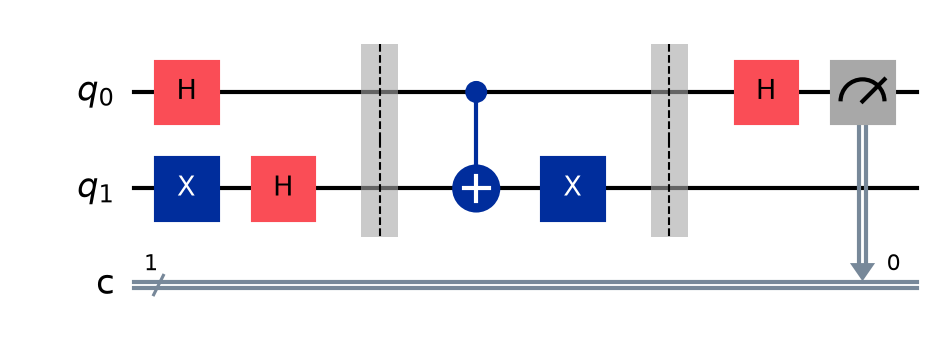
\includegraphics[width=0.55\textwidth]{deutsch_circuito.png}

\small El circuito de Deutsch para $f_3$ dibujado por Qiskit. Entre las dos barreras está el oráculo: un CNOT ($x$ controla $y$) y una $X$ sobre $y$. El cable de arriba es $\mathsf{q}_0 = x$.
\end{cajafigura}

\noindent Con $1000$ disparos para cada función se obtiene:
\begin{codigo}[language={}]
f1 {'0': 1000}
f2 {'1': 1000}
f3 {'1': 1000}
f4 {'0': 1000}
\end{codigo}

\begin{cajafigura}
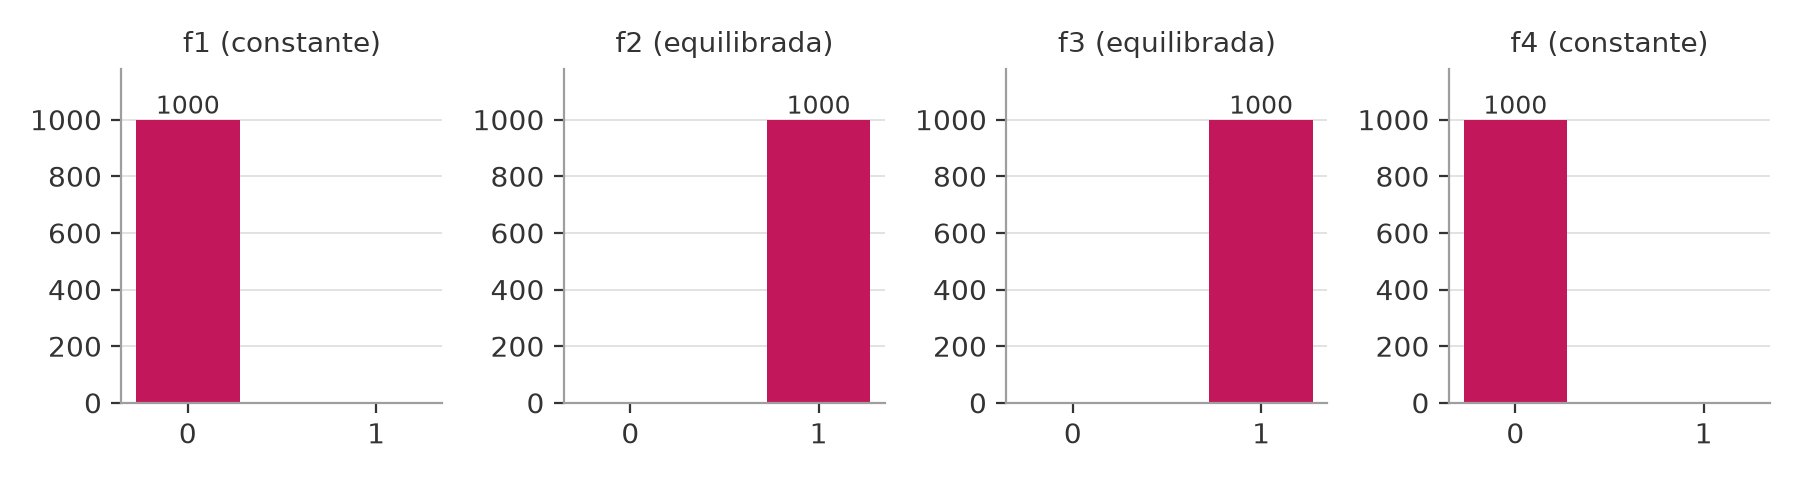
\includegraphics[width=\textwidth]{deutsch_histogramas.png}

\small Resultados del algoritmo de Deutsch con $1000$ disparos. Las funciones constantes dan siempre $0$ y las equilibradas siempre $1$, sin un solo error: el algoritmo es \textbf{determinista}, no probabilístico.
\end{cajafigura}

\noindent Por último, comprobamos el estado final exacto para $f_3$ (quitando la medición):
\begin{codigo}
qc = deutsch("f3").remove_final_measurements(inplace=False)
psi = Statevector.from_label("00").evolve(qc)
print(np.round(psi.data.real * sqrt(2), 3))      # [-0. -1.  0.  1.]
\end{codigo}
\noindent El vector $\frac{1}{\sqrt2}(0, -1, 0, 1)$ en la base $\ket{00},\ket{01},\ket{10},\ket{11}$ es $\frac{1}{\sqrt2}(-\ket{01}+\ket{11}) = -\ket{-}\ket{1}$, el resultado del Ejercicio 6.1.6.

\cleardoublepage
\section{Resumen: un ejemplo guiado}

\noindent Seguimos una sola función, la del ejemplo del libro: $f = f_3$, con $f(0) = 1$ y $f(1) = 0$ (NOT). En cada caja, la parte superior es el cálculo y la inferior, el concepto.

\pasoguiado{Paso 1. El problema}
{$f(0) = 1$, $f(1) = 0$, pero no lo sabemos: solo podemos consultar $f$. ¿Es constante o equilibrada?}
{\textbf{Problema de Deutsch:} decidir si $f(0)\oplus f(1)$ vale $0$ (constante) o $1$ (equilibrada). \textbf{Modelo de consultas:} el coste es el número de evaluaciones de $f$.}

\pasoguiado{Paso 2. Clásicamente, dos consultas}
{Consultamos $f(0) = 1$. Siguen siendo posibles $f_4$ (constante) y $f_3$ (equilibrada). Hay que consultar también $f(1)$.}
{Ningún algoritmo clásico determinista lo resuelve con una consulta.}

\pasoguiado{Paso 3. El oráculo}
{$U_f\ket{y}\ket{x} = \ket{y\oplus f(x)}\ket{x}$: \; $U_f\ket{00} = \ket{10}$, \; $U_f\ket{01} = \ket{01}$, \; $U_f\ket{10} = \ket{00}$, \; $U_f\ket{11} = \ket{11}$.}
{\textbf{Oráculo:} evalúa $f$ de forma reversible guardando la entrada y haciendo XOR en la salida. Es una permutación, $U_f^2 = I$, y es unitaria aunque $f$ no sea invertible.}

\pasoguiado{Paso 4. Primer intento}
{$U_f\,\ket{0}\ket{+} = \tfrac{1}{\sqrt2}(\ket{10}+\ket{01})$: al medir sale $(y, x) = (1, 0)$ o $(0, 1)$, cada uno con probabilidad $\frac12$.}
{\textbf{Superposición sin interferencia} equivale a consultar una entrada al azar: no basta.}

\pasoguiado{Paso 5. El retroceso de fase}
{$U_f\ket{-}\ket{0} = -\ket{-}\ket{0}$ \;(pues $f(0) = 1$), \qquad $U_f\ket{-}\ket{1} = +\ket{-}\ket{1}$ \;(pues $f(1) = 0$).}
{\textbf{Retroceso de fase:} con la salida en $\ket{-}$, el oráculo multiplica $\ket{x}$ por $(-1)^{f(x)}$ y deja la salida igual.}

\pasoguiado{Paso 6. Superposición}
{$\ket{\varphi_1} = (H\otimes H)\ket{1}\ket{0} = \ket{-}\ket{+} = \tfrac12(\ket{00}+\ket{01}-\ket{10}-\ket{11})$.}
{Las Hadamard ponen la entrada en superposición de las dos entradas y la salida en $\ket{-}$. \textbf{Orden de Qiskit:} la salida $y$ (abajo) es el factor de la izquierda.}

\pasoguiado{Paso 7. Una consulta}
{$\ket{\varphi_2} = \ket{-}\otimes\tfrac{1}{\sqrt2}\big(-\ket{0}+\ket{1}\big) = -\ket{-}\ket{-}$.}
{Cada componente recibe su signo: la información sobre $f$ está ahora en una \textbf{fase relativa}. El estado es un \textbf{producto}: no hay entrelazamiento.}

\pasoguiado{Paso 8. Interferencia}
{$\ket{\varphi_3} = (I\otimes H)\ket{\varphi_2} = -\ket{-}\ket{1}$, porque $H\ket{-} = \ket{1}$: las amplitudes de $\ket{0}$ se cancelan ($\tfrac12 - \tfrac12 = 0$).}
{\textbf{Interferencia:} la Hadamard final convierte la fase relativa en un resultado de la base estándar. Es un \textbf{cambio de base}.}

\pasoguiado{Paso 9. Medir}
{Se obtiene $1$ con probabilidad $|-1|^2 = 1$: $f$ es equilibrada. Qiskit: \texttt{\{'1': 1000\}}.}
{El resultado es $f(0)\oplus f(1)$ con certeza y \textbf{una sola consulta}. El signo $-1$ (que distinguiría $f_3$ de $f_2$) es una fase global: no se observa.}

\begin{center}
\small\renewcommand{\arraystretch}{1.15}
\begin{tabular}{c|l|l}
\textbf{Paso} & \textbf{Qué hicimos} & \textbf{Concepto} \\ \hline
1 & ¿Constante o equilibrada? & Problema de Deutsch, modelo de consultas \\
2 & Consultar $f(0)$ & Cota clásica: dos consultas \\
3 & $U_f\ket{y}\ket{x} = \ket{y\oplus f(x)}\ket{x}$ & Oráculo reversible y unitario \\
4 & Entrada en $\ket{+}$ & Superposición sin interferencia no basta \\
5 & Salida en $\ket{-}$ & Retroceso de fase \\
6 & $H\otimes H$ & Superposición; orden de Qiskit \\
7 & Aplicar $U_f$ & Información en la fase relativa \\
8 & $H$ arriba & Interferencia, cambio de base \\
9 & Medir & $f(0)\oplus f(1)$ con certeza, una consulta
\end{tabular}
\end{center}

% =====================================================================
\chapter{El algoritmo de Deutsch--Jozsa}

\noindent El algoritmo de Deutsch--Jozsa \cite{deutsch1992, cleve1998} generaliza el de Deutsch a funciones de $n$ bits. Con una sola consulta distingue una función constante de una equilibrada, mientras que un algoritmo clásico determinista necesita $2^{n-1}+1$ consultas: es el primer ejemplo de \textbf{ventaja exponencial}. La herramienta nueva es la transformada de Hadamard de $n$ qubits, $H^{\otimes n}$, que aparecerá en todos los capítulos siguientes. Corresponde a la sección 6.2 de Yanofsky.

\cleardoublepage
\section{El problema y la solución clásica}

\noindent Consideramos funciones $f:\bits{n}\to\{0,1\}$, que reciben una cadena de $n$ bits y devuelven un bit. Escribimos las cadenas en negrita, $\bx\in\bits{n}$, y a menudo las identificamos con el número natural que representan en binario, de $0$ a $2^n-1$.

\begin{teoria}{Definición: funciones constantes y equilibradas}
Una función $f:\bits{n}\to\{0,1\}$ es \textbf{constante} si toma el mismo valor en todas las entradas, y \textbf{equilibrada} si toma el valor $0$ en exactamente la mitad de las entradas ($2^{n-1}$) y el valor $1$ en la otra mitad.
\end{teoria}

\begin{ejercicio}{Ejercicio 6.2.1 (Yanofsky): ¿cuántas funciones hay?}
\textbf{Todas.} Para cada una de las $2^n$ entradas hay que elegir una salida entre dos: hay $2^{2^n}$ funciones.

\textbf{Equilibradas.} Una función equilibrada queda determinada por el conjunto de las $2^{n-1}$ entradas que van a $1$, que es un subconjunto de tamaño $2^{n-1}$ de un conjunto de $2^n$ elementos: hay $\binom{2^n}{2^{n-1}}$.

\textbf{Constantes.} Exactamente $2$: la constante $0$ y la constante $1$.
\[
\renewcommand{\arraystretch}{1.2}
\begin{array}{c|r|r|r|r}
n & \text{funciones} & \text{equilibradas} & \text{constantes} & \text{ninguna de las dos} \\ \hline
1 & 4 & 2 & 2 & 0 \\
2 & 16 & 6 & 2 & 8 \\
3 & 256 & 70 & 2 & 184 \\
4 & 65\,536 & 12\,870 & 2 & 52\,664
\end{array}
\]
Para $n\ge2$ la mayoría de las funciones no son ni constantes ni equilibradas: el problema solo tiene sentido con la \textbf{promesa} de que $f$ es de uno de los dos tipos.
\end{ejercicio}

\begin{teoria}{El problema de Deutsch--Jozsa}
Se da $f:\bits{n}\to\{0,1\}$ como caja negra, con la \textbf{promesa} de que es constante o equilibrada. Hay que decidir cuál de las dos cosas es. Para $n = 1$ es el problema de Deutsch.
\end{teoria}

\begin{teoria}{Proposición: cota clásica}
Todo algoritmo clásico determinista que resuelva el problema sin error necesita, en el peor caso, $2^{n-1}+1$ consultas, y con ese número basta.
\end{teoria}

\begin{demo}
\textit{Bastan.} Se consulta $f$ en $2^{n-1}+1$ entradas distintas. Si aparecen dos valores distintos, $f$ no es constante, luego es equilibrada. Si todos coinciden, $f$ toma el mismo valor en más de la mitad de las entradas, luego no es equilibrada, y por la promesa es constante.

\textit{Hacen falta.} Supongamos que un algoritmo hace como mucho $2^{n-1}$ consultas. Lo enfrentamos a un ``adversario'' que responde $0$ a todas. Al terminar, el algoritmo ha visto a lo sumo $2^{n-1}$ ceros. Hay entonces dos funciones compatibles con todo lo que ha visto: la constante $0$, y una función equilibrada que vale $0$ en las entradas consultadas (y en otras, si hacen falta para completar $2^{n-1}$ ceros) y $1$ en las $2^{n-1}$ restantes. La segunda existe porque se han consultado como mucho $2^{n-1}$ entradas. Las dos funciones producen la misma ejecución, así que el algoritmo da la misma respuesta para ambas y falla en una. \hfill$\square$
\end{demo}

\begin{aclaracion}{Nota Aclaratoria: la ventaja exponencial es frente a algoritmos exactos}
Si se permite un pequeño error, un algoritmo clásico \textbf{aleatorio} lo hace muy bien: se consultan $k$ entradas elegidas al azar y se responde ``constante'' si todas coinciden. Si $f$ es constante, nunca falla. Si $f$ es equilibrada, cada consulta da $0$ o $1$ con probabilidad $\frac12$ cada uno, de forma independiente, así que la probabilidad de que las $k$ coincidan es $2\cdot(\tfrac12)^k = 2^{1-k}$; con $k = 11$ consultas el error es menor que $0{,}001$ para todo $n$. La ventaja exponencial de Deutsch--Jozsa es, por tanto, frente a algoritmos clásicos que no se equivocan nunca. En el Capítulo~3 (Simon) la ventaja sobrevivirá también frente a los algoritmos aleatorios.
\end{aclaracion}

\cleardoublepage
\section{El algoritmo cuántico}

\subsection{El oráculo de $n$ qubits}

\noindent El oráculo se define igual que en el Capítulo~1, ahora con un registro de entrada de $n$ qubits \Yan{6.44}:
\[ U_f\big(\ket{y}\ket{\bx}\big) = \ket{y\oplus f(\bx)}\ket{\bx}, \qquad \bx\in\bits{n},\; y\in\{0,1\}. \]
\begin{center}
\begin{quantikz}
\lstick{$\ket{\bx}$} & \qwbundle{n} & \gate[2]{U_f} & \rstick{$\ket{\bx}$} \\
\lstick{$\ket{y}$} & & & \rstick{$\ket{y\oplus f(\bx)}$}
\end{quantikz}
\end{center}
La barra con una $n$ indica un registro de $n$ qubits. En Qiskit, $\bx$ ocupa $\mathsf{q}_0,\dots,\mathsf{q}_{n-1}$ y $y$ es $\mathsf{q}_n$, de modo que el índice de $\ket{y}\ket{\bx}$ en la base es $y\cdot2^n + \bx$. La demostración del Capítulo~1 se aplica literalmente: $U_f$ es una permutación, $U_f^2 = I$ y $U_f$ es unitaria.

\begin{ejemplo}{Ejemplo 6.2.1 (Yanofsky): el oráculo de una función equilibrada de 2 bits}
La función de \Yan{6.45} es
\[ f(\texttt{00}) = 1, \quad f(\texttt{01}) = 1, \quad f(\texttt{10}) = 0, \quad f(\texttt{11}) = 0, \]
equilibrada (dos ceros y dos unos). En el orden de Qiskit, con la base ordenada como $\ket{y\,x_1x_0}$ de $\ket{000}$ a $\ket{111}$, el oráculo intercambia $\ket{0}\ket{\bx}\leftrightarrow\ket{1}\ket{\bx}$ cuando $f(\bx) = 1$ y deja fijos los demás vectores:
\[
U_f:\quad \ket{000}\leftrightarrow\ket{100}, \qquad \ket{001}\leftrightarrow\ket{101}, \qquad \ket{010}, \ket{011}, \ket{110}, \ket{111} \text{ fijos},
\]
\[
U_f = \begin{array}{c} \scriptstyle 000\\ \scriptstyle 001\\ \scriptstyle 010\\ \scriptstyle 011\\ \scriptstyle 100\\ \scriptstyle 101\\ \scriptstyle 110\\ \scriptstyle 111 \end{array}
\!\!\begin{pmatrix}
\cdot&\cdot&\cdot&\cdot&1&\cdot&\cdot&\cdot\\
\cdot&\cdot&\cdot&\cdot&\cdot&1&\cdot&\cdot\\
\cdot&\cdot&1&\cdot&\cdot&\cdot&\cdot&\cdot\\
\cdot&\cdot&\cdot&1&\cdot&\cdot&\cdot&\cdot\\
1&\cdot&\cdot&\cdot&\cdot&\cdot&\cdot&\cdot\\
\cdot&1&\cdot&\cdot&\cdot&\cdot&\cdot&\cdot\\
\cdot&\cdot&\cdot&\cdot&\cdot&\cdot&1&\cdot\\
\cdot&\cdot&\cdot&\cdot&\cdot&\cdot&\cdot&1
\end{pmatrix}
\]
(los puntos son ceros). La matriz \Yan{6.46} del libro intercambia $\ket{00,0}\leftrightarrow\ket{00,1}$ y $\ket{01,0}\leftrightarrow\ket{01,1}$: son los mismos pares de estados con el qubit $y$ escrito a la derecha.
\end{ejemplo}

\begin{ejercicio}{Ejercicios 6.2.2 y 6.2.3 (Yanofsky)}
\textbf{6.2.2.} La función de \Yan{6.47} es $f(\texttt{00}) = f(\texttt{01}) = 0$, $f(\texttt{10}) = f(\texttt{11}) = 1$ (equilibrada; $f(\bx)$ es el primer bit por la izquierda de $\bx$). Su oráculo intercambia
\[ \ket{010}\leftrightarrow\ket{110}, \qquad \ket{011}\leftrightarrow\ket{111}, \]
y deja fijos $\ket{000}, \ket{001}, \ket{100}, \ket{101}$. Es un CNOT con control en $\mathsf{q}_1$ y objetivo en $y = \mathsf{q}_2$.

\textbf{6.2.3.} Para la constante $1$, el oráculo cambia siempre $y$: $\ket{0}\ket{\bx}\leftrightarrow\ket{1}\ket{\bx}$ para los cuatro $\bx$. Es $X\otimes I\otimes I$, la matriz con dos bloques identidad $4\times4$ fuera de la diagonal, $\left(\begin{smallmatrix} 0 & I_4\\ I_4 & 0\end{smallmatrix}\right)$.
\end{ejercicio}

\subsection{La transformada de Hadamard de $n$ qubits}

\noindent Para poner $n$ qubits en superposición se aplica una Hadamard a cada uno, es decir, la matriz $H^{\otimes n} = H\otimes\cdots\otimes H$. Yanofsky busca el patrón calculando $H$, $H^{\otimes2}$ y $H^{\otimes3}$ \Yan{6.48--6.60}. La clave es escribir las entradas de $H$ como potencias de $-1$:
\[ H = \frac{1}{\sqrt2}\begin{pmatrix} 1 & 1 \\ 1 & -1 \end{pmatrix}, \qquad H_{ij} = \frac{1}{\sqrt2}(-1)^{ij}, \quad i,j\in\{0,1\}, \]
pues el producto $ij$ de dos bits (que es su AND) solo vale $1$ en la esquina inferior derecha.

\begin{teoria}{Definición: producto binario de cadenas}
Para $\bx, \bz\in\bits{n}$,
\[ \bx\cdot\bz = x_{n-1}z_{n-1}\oplus\cdots\oplus x_1z_1\oplus x_0z_0 \in\{0,1\}, \qquad \text{(Yanofsky: } \langle\bx,\bz\rangle\text{, \Yan{6.54}).} \]
Es la paridad del número de posiciones en que $\bx$ y $\bz$ valen $1$ a la vez. Escribimos también $\bx\oplus\bz$ para el XOR bit a bit \Yan{6.55} y $\bcero$ para la cadena de $n$ ceros.
\end{teoria}

\begin{teoria}{Proposición: propiedades del producto binario}
Para $\bx, \bx', \bz, \bz'\in\bits{n}$:
\begin{enumerate}
\item $(\bx\oplus\bx')\cdot\bz = (\bx\cdot\bz)\oplus(\bx'\cdot\bz)$ y $\bx\cdot(\bz\oplus\bz') = (\bx\cdot\bz)\oplus(\bx\cdot\bz')$ \;\Yan{6.56, 6.57};
\item $\bcero\cdot\bz = \bx\cdot\bcero = 0$ \;\Yan{6.58, 6.59};
\item $\bx\cdot\bz = \bz\cdot\bx$;
\item $(-1)^{a}(-1)^{b} = (-1)^{a\oplus b}$ para bits $a, b$.
\end{enumerate}
\end{teoria}

\begin{demo}
Las propiedades 2 y 3 son inmediatas. Para la 4: $a + b$ y $a\oplus b$ solo difieren cuando $a = b = 1$ ($2$ frente a $0$), y ambos números son pares, así que $(-1)^{a+b} = (-1)^{a\oplus b}$. Para la 1, en cada posición $(x_k\oplus x'_k)z_k = x_kz_k\oplus x'_kz_k$ (es la distributividad en $\F$: basta comprobar los ocho casos o notar que, si $z_k = 0$, los dos lados valen $0$, y si $z_k = 1$, los dos valen $x_k\oplus x'_k$); sumando con $\oplus$ las $n$ posiciones y reordenando (la operación $\oplus$ es asociativa y conmutativa) se obtiene la igualdad. La segunda igualdad se sigue de la primera y de la simetría.

\textit{Comentario.} Como observa Yanofsky en una nota a pie de página, $\bits{n}$ con $\oplus$ es un espacio vectorial sobre el cuerpo de dos elementos $\F = \{0,1\}$, y $\bx\cdot\bz$ es una forma bilineal simétrica sobre él. Esta estructura será esencial en el Capítulo~3. \hfill$\square$
\end{demo}

\begin{teoria}{Teorema: fórmula de $H^{\otimes n}$}
Para todo $n\ge1$ y todas las cadenas $\bz$ (fila) y $\bx$ (columna),
\[ \big(H^{\otimes n}\big)_{\bz\bx} = \frac{1}{\sqrt{2^n}}\,(-1)^{\bx\cdot\bz}. \qquad \Yan{6.61} \]
Equivalentemente, para cada cadena $\bx$,
\[ H^{\otimes n}\ket{\bx} = \frac{1}{\sqrt{2^n}}\sum_{\bz\in\bits{n}}(-1)^{\bx\cdot\bz}\ket{\bz} \qquad \Yan{6.64} \]
y, en particular,
\[ H^{\otimes n}\ket{\bcero} = \frac{1}{\sqrt{2^n}}\sum_{\bz\in\bits{n}}\ket{\bz}. \qquad \Yan{6.63} \]
\end{teoria}

\begin{demo}
Por inducción sobre $n$ (esto resuelve también el Ejercicio 6.2.4, que pide probar que el factor es $2^{-n/2}$). Para $n = 1$ es la fórmula $H_{ij} = \frac{1}{\sqrt2}(-1)^{ij}$.

Supongamos la fórmula cierta para $n$. Escribimos una cadena de $n+1$ bits como $\bx = x_n\bx'$, con $x_n$ el bit de la izquierda y $\bx'$ los $n$ restantes, y $H^{\otimes(n+1)} = H\otimes H^{\otimes n}$. Por la definición del producto de Kronecker, la entrada en la fila $z_n\bz'$ y la columna $x_n\bx'$ es el producto de la entrada $(z_n, x_n)$ del primer factor por la entrada $(\bz', \bx')$ del segundo:
\begin{align*}
\big(H^{\otimes(n+1)}\big)_{\bz\bx} &= H_{z_nx_n}\,\big(H^{\otimes n}\big)_{\bz'\bx'} = \frac{1}{\sqrt2}(-1)^{x_nz_n}\cdot\frac{1}{\sqrt{2^n}}(-1)^{\bx'\cdot\bz'} \\
&= \frac{1}{\sqrt{2^{n+1}}}(-1)^{x_nz_n\oplus\,\bx'\cdot\bz'} = \frac{1}{\sqrt{2^{n+1}}}(-1)^{\bx\cdot\bz},
\end{align*}
usando la propiedad 4 y que $\bx\cdot\bz = x_nz_n\oplus\bx'\cdot\bz'$ por definición. Esto prueba la fórmula para $n+1$.

La segunda forma es la primera leída por columnas: $H^{\otimes n}\ket{\bx}$ es la columna $\bx$, cuya entrada $\bz$ es $2^{-n/2}(-1)^{\bx\cdot\bz}$. Con $\bx = \bcero$, todos los signos son $+1$ por la propiedad 2. \hfill$\square$
\end{demo}

\begin{aclaracion}{Nota Aclaratoria: la fórmula no depende del orden de los qubits}
$H^{\otimes n}$ es la misma matriz con la convención de Yanofsky y con la de Qiskit, porque todos sus factores son iguales; y $\bx\cdot\bz$ no cambia si se reordenan a la vez las posiciones de $\bx$ y de $\bz$. Por eso la fórmula \Yan{6.61} se puede usar tal cual. Además, $H^{\otimes n}$ es real y simétrica (pues $\bx\cdot\bz = \bz\cdot\bx$) y $(H^{\otimes n})^2 = (H^2)^{\otimes n} = I$.
\end{aclaracion}

\begin{ejemplo}{Ejemplo: $H^{\otimes2}$ y $H^{\otimes3}$ con números}
Con filas y columnas ordenadas de $\texttt{00}$ a $\texttt{11}$, \Yan{6.51}:
\[ H^{\otimes2} = \frac12\begin{pmatrix} 1&1&1&1\\1&-1&1&-1\\1&1&-1&-1\\1&-1&-1&1 \end{pmatrix}. \]
Comprobación de una entrada con la fórmula: fila $\texttt{11}$, columna $\texttt{01}$: $\texttt{01}\cdot\texttt{11} = 0\oplus1 = 1$, así que la entrada es $\frac12(-1)^1 = -\frac12$. Es la cuarta fila y segunda columna, en efecto $-\frac12$.

Para $n = 3$, $\sqrt8\,H^{\otimes3}$ es \Yan{6.60}
\[
\begin{pmatrix}
1&1&1&1&1&1&1&1\\ 1&-1&1&-1&1&-1&1&-1\\ 1&1&-1&-1&1&1&-1&-1\\ 1&-1&-1&1&1&-1&-1&1\\
1&1&1&1&-1&-1&-1&-1\\ 1&-1&1&-1&-1&1&-1&1\\ 1&1&-1&-1&-1&-1&1&1\\ 1&-1&-1&1&-1&1&1&-1
\end{pmatrix}.
\]
Cada fila salvo la primera tiene cuatro $+1$ y cuatro $-1$: \textbf{suma cero}. Este hecho es el lema siguiente.
\end{ejemplo}

\begin{teoria}{Lema: suma de signos}
Para todo $\bz\in\bits{n}$,
\[ \sum_{\bx\in\bits{n}}(-1)^{\bx\cdot\bz} = \begin{cases} 2^n & \text{si } \bz = \bcero, \\ 0 & \text{si } \bz\neq\bcero. \end{cases} \]
\end{teoria}

\begin{demo}
Si $\bz = \bcero$, todos los sumandos valen $1$. Si $\bz\neq\bcero$, hay una posición $k$ con $z_k = 1$; sea $\mathbf{e}_k$ la cadena con un $1$ solo en la posición $k$. La aplicación $\bx\mapsto\bx\oplus\mathbf{e}_k$ es una biyección de $\bits{n}$ en sí mismo que agrupa las cadenas en parejas $\{\bx, \bx\oplus\mathbf{e}_k\}$. Por la propiedad 1, $(\bx\oplus\mathbf{e}_k)\cdot\bz = \bx\cdot\bz\oplus z_k = \bx\cdot\bz\oplus1$: los dos miembros de cada pareja tienen signos opuestos y se cancelan. La suma total es $0$. \hfill$\square$
\end{demo}

\noindent El lema dice que las columnas de $\sqrt{2^n}\,H^{\otimes n}$ son ortogonales a la primera, que es el vector de unos. Es otra forma de ver que $H^{\otimes n}$ es unitaria.

\subsection{Primer intento}

\noindent Como en el Capítulo~1, si la entrada es un estado de la base $\ket{\bx}$ y la salida está en $\ket{-}$ \Yan{6.65}, el lema del retroceso de fase (cuya demostración no usa que $x$ sea un solo bit) da
\[ U_f\big(\ket{-}\ket{\bx}\big) = (-1)^{f(\bx)}\ket{-}\ket{\bx}. \qquad \Yan{6.70} \]
Es una fase global y no da información. Hay que poner la entrada en superposición.

\subsection{El algoritmo}

\begin{center}
\begin{quantikz}
\lstick{$\ket{\bcero}$ \;($\bx$)} & \qwbundle{n} \slice{$\ket{\varphi_0}$} & \gate{H^{\otimes n}} \slice{$\ket{\varphi_1}$} & \gate[2]{U_f} \slice{$\ket{\varphi_2}$} & \gate{H^{\otimes n}} \slice{$\ket{\varphi_3}$} & \meter{} & \setwiretype{c} \\
\lstick{$\ket{1}$ \;($y$)} & & \gate{H} & & & &
\end{quantikz}
\end{center}
En matrices, con el orden de Qiskit, $\ket{\varphi_3} = (I\otimes H^{\otimes n})\,U_f\,(H\otimes H^{\otimes n})\,\ket{1}\ket{\bcero}$.

\begin{convencion}{la fórmula del algoritmo}
El libro escribe \Yan{6.72} $(H^{\otimes n}\otimes I)\,U_f\,(H^{\otimes n}\otimes H)\ket{\bcero,1}$: los factores de cada producto tensorial aparecen en el orden contrario al nuestro, por la misma razón que en el Capítulo~1.
\end{convencion}

\begin{teoria}{Teorema: corrección del algoritmo de Deutsch--Jozsa}
Para toda $f:\bits{n}\to\{0,1\}$,
\[ \ket{\varphi_3} = \ket{-}\otimes\sum_{\bz\in\bits{n}} a_{\bz}\ket{\bz}, \qquad a_{\bz} = \frac{1}{2^n}\sum_{\bx\in\bits{n}}(-1)^{f(\bx)\oplus\,\bx\cdot\bz}. \]
En particular, la probabilidad de obtener $\bcero$ al medir el registro de arriba es
\[ \Pr(\bcero) = \left(\frac{1}{2^n}\sum_{\bx}(-1)^{f(\bx)}\right)^2 = \left(\frac{N_0 - N_1}{2^n}\right)^2, \]
donde $N_0$ y $N_1$ son el número de entradas con $f(\bx) = 0$ y $f(\bx) = 1$. Por tanto:
\begin{itemize}
\item si $f$ es \textbf{constante}, se obtiene $\bcero$ con probabilidad $1$;
\item si $f$ es \textbf{equilibrada}, se obtiene $\bcero$ con probabilidad $0$.
\end{itemize}
Basta \textbf{una consulta} y el resultado es seguro: se responde ``constante'' si y solo si se mide $\bcero$.
\end{teoria}

\begin{demo}
\textit{Paso 0.} $\ket{\varphi_0} = \ket{1}\ket{\bcero}$.

\textit{Paso 1.} Por el teorema de $H^{\otimes n}$, $\ket{\varphi_1} = H\ket{1}\otimes H^{\otimes n}\ket{\bcero} = \ket{-}\otimes\frac{1}{\sqrt{2^n}}\sum_{\bx}\ket{\bx}$ \Yan{6.74}.

\textit{Paso 2.} Por linealidad y el retroceso de fase, $\ket{\varphi_2} = \ket{-}\otimes\frac{1}{\sqrt{2^n}}\sum_{\bx}(-1)^{f(\bx)}\ket{\bx}$ \Yan{6.75}.

\textit{Paso 3.} Aplicando $H^{\otimes n}$ a cada $\ket{\bx}$ con la fórmula del teorema \Yan{6.76}:
\[ \ket{\varphi_3} = \ket{-}\otimes\frac{1}{\sqrt{2^n}}\sum_{\bx}(-1)^{f(\bx)}\,\frac{1}{\sqrt{2^n}}\sum_{\bz}(-1)^{\bx\cdot\bz}\ket{\bz} = \ket{-}\otimes\sum_{\bz}\Big(\frac{1}{2^n}\sum_{\bx}(-1)^{f(\bx)\oplus\,\bx\cdot\bz}\Big)\ket{\bz}, \]
intercambiando las sumas (finitas) y usando la propiedad 4. Esto es \Yan{6.77}.

\textit{Medición.} El estado es un producto con el qubit de abajo en $\ket{-}$, así que la probabilidad de obtener $\bz$ arriba es $|a_{\bz}|^2$. Para $\bz = \bcero$, $\bx\cdot\bcero = 0$ y $a_{\bcero} = \frac{1}{2^n}\sum_{\bx}(-1)^{f(\bx)} = \frac{N_0 - N_1}{2^n}$, pues cada entrada con $f(\bx) = 0$ aporta $+1$ y cada una con $f(\bx) = 1$ aporta $-1$. Si $f$ es constante, $N_0 - N_1 = \pm2^n$ y $a_{\bcero} = \pm1$ \Yan{6.79, 6.80}; como $\sum_{\bz}|a_{\bz}|^2 = 1$, las demás amplitudes son $0$ y se obtiene $\bcero$ con certeza. Si $f$ es equilibrada, $N_0 = N_1$ y $a_{\bcero} = 0$ \Yan{6.81}. \hfill$\square$
\end{demo}

\begin{ejercicio}{Ejercicio 6.2.5 (Yanofsky): ¿y si nos engañan?}
Si $f$ no es ni constante ni equilibrada, el teorema sigue valiendo: se obtiene $\bcero$ con probabilidad $\big((N_0 - N_1)/2^n\big)^2$, que está \textbf{estrictamente} entre $0$ y $1$ (no es $0$ porque $N_0\neq N_1$, ni $1$ porque $|N_0-N_1| < 2^n$). El algoritmo responde a veces ``constante'' y a veces ``equilibrada'', sin que ninguna respuesta tenga sentido.

Ejemplo: $f = \mathrm{AND}$ de dos bits, $f(\texttt{11}) = 1$ y $f = 0$ en las otras tres entradas. Entonces $N_0 = 3$, $N_1 = 1$ y $\Pr(\texttt{00}) = (2/4)^2 = \frac14$. Las cuatro amplitudes son
\[ a_{\bz} = \tfrac14\big(1 + (-1)^{\texttt{01}\cdot\bz} + (-1)^{\texttt{10}\cdot\bz} - (-1)^{\texttt{11}\cdot\bz}\big): \qquad a_{\texttt{00}} = a_{\texttt{01}} = a_{\texttt{10}} = \tfrac12, \quad a_{\texttt{11}} = -\tfrac12, \]
así que los cuatro resultados salen con probabilidad $\frac14$ (Experimento 2).
\end{ejercicio}

\begin{ejemplo}{Ejemplo completo: la función equilibrada \Yan{6.45}}
Sea $f(\texttt{00}) = f(\texttt{01}) = 1$, $f(\texttt{10}) = f(\texttt{11}) = 0$, con $n = 2$.
\begin{align*}
\ket{\varphi_0} &= \ket{1}\ket{00}, \\
\ket{\varphi_1} &= \ket{-}\otimes\tfrac12\big(\ket{00}+\ket{01}+\ket{10}+\ket{11}\big), \\
\ket{\varphi_2} &= \ket{-}\otimes\tfrac12\big(-\ket{00}-\ket{01}+\ket{10}+\ket{11}\big).
\end{align*}
Para $\ket{\varphi_3}$ calculamos las cuatro amplitudes $a_{\bz} = \frac14\sum_{\bx}(-1)^{f(\bx)}(-1)^{\bx\cdot\bz}$, es decir, el producto de la fila $\bz$ de $2H^{\otimes2}$ por el vector de signos $(-1,-1,+1,+1)$:
\[
a_{\texttt{00}} = \tfrac14(-1-1+1+1) = 0, \quad
a_{\texttt{01}} = \tfrac14(-1+1+1-1) = 0, \]
\[
a_{\texttt{10}} = \tfrac14(-1-1-1-1) = -1, \quad
a_{\texttt{11}} = \tfrac14(-1+1-1+1) = 0.
\]
Así $\ket{\varphi_3} = -\ket{-}\ket{10}$: se mide $\texttt{10}$ con certeza. Como no es $\texttt{00}$, $f$ es equilibrada.

\textit{Por qué sale justo $\texttt{10}$:} $(-1)^{f(\bx)} = -(-1)^{x_1}$, donde $x_1$ es el primer bit por la izquierda, y $(-1)^{x_1} = (-1)^{\bx\cdot\texttt{10}}$. El vector de signos es, salvo el signo global, una columna de $2H^{\otimes2}$, y la Hadamard la devuelve al vector de la base $\ket{\texttt{10}}$.
\end{ejemplo}

\begin{tfg}
La amplitud que decide el algoritmo es un \textbf{producto interno}. Con $\ket{s} = H^{\otimes n}\ket{\bcero}$ y la matriz diagonal de signos $Z_f = \sum_{\bx}(-1)^{f(\bx)}\ket{\bx}\bra{\bx}$,
\[ a_{\bcero} = \bra{\bcero}H^{\otimes n}Z_fH^{\otimes n}\ket{\bcero} = \braket{s}{Z_f\,s}, \qquad \Pr(\bcero) = |\braket{s}{Z_f\,s}|^2. \]
Es una \textbf{fidelidad} entre los estados $\ket{s}$ y $Z_f\ket{s}$, y se estima exactamente como el kernel cuántico $K(\mathbf{x},\mathbf{y}) = |\braket{\phi(\mathbf{x})}{\phi(\mathbf{y})}|^2$: preparando un estado, deshaciendo otro y midiendo la frecuencia de $\ket{0\cdots0}$ (Capítulo~3 del cuaderno). En el \texttt{ZZFeatureMap} de Havlíček et al.\ \cite{havlicek2019supervised}, $Z_f$ se sustituye por una matriz diagonal de fases $e^{i\phi(\mathbf{x})}$ que dependen del dato.
\end{tfg}

\cleardoublepage
\section{Implementación en Qiskit}

\subsection{Un oráculo para cualquier función}

\noindent Para funciones de varios bits construimos $U_f$ directamente a partir de su definición, como matriz de permutación. La función recibe y devuelve enteros, que son las cadenas de bits leídas en binario al modo de Qiskit:
\begin{codigo}
def oraculo(f, n, m, etiqueta="U_f"):
    """U_f |y>|x> = |y xor f(x)>|x>: x en los n primeros qubits, y en los m siguientes."""
    N = 2 ** (n + m)
    U = np.zeros((N, N))
    for x in range(2 ** n):
        for y in range(2 ** m):
            U[(y ^ f(x)) * 2 ** n + x, y * 2 ** n + x] = 1
    return UnitaryGate(U, label=etiqueta)
\end{codigo}
\noindent La entrada $(\text{fila}, \text{columna}) = \big((y\oplus f(x))\,2^n + x,\; y\,2^n + x\big)$ es exactamente ``la columna de $\ket{y}\ket{\bx}$ tiene su $1$ en la fila de $\ket{y\oplus f(\bx)}\ket{\bx}$''. Al añadir la puerta con \texttt{qc.append(oraculo(...), range(n + m))}, el primer qubit de la lista es el bit menos significativo del índice, de acuerdo con el orden de Qiskit. (Construir así el oráculo no es eficiente para $n$ grande, pues la matriz tiene $4^{n+m}$ entradas, pero es perfecto para comprobar el algoritmo; en el Capítulo~4 se construye uno con puertas.)

\subsection{Experimento 2: Deutsch--Jozsa con funciones de 2 bits}

\begin{codigo}
def deutsch_jozsa(f, n):
    qc = QuantumCircuit(n + 1, n)
    qc.x(n)
    qc.h(range(n + 1))
    qc.barrier()
    qc.append(oraculo(f, n, 1), range(n + 1))
    qc.barrier()
    qc.h(range(n))
    qc.measure(range(n), range(n))
    return qc
\end{codigo}

\begin{cajafigura}
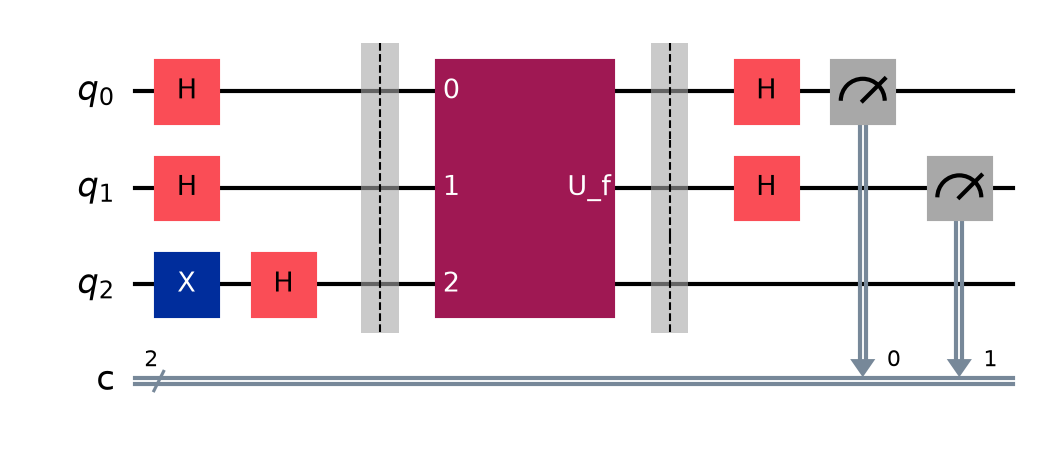
\includegraphics[width=0.58\textwidth]{dj_circuito.png}

\small El circuito de Deutsch--Jozsa con $n = 2$: $\mathsf{q}_0, \mathsf{q}_1$ forman el registro $\bx$ y $\mathsf{q}_2$ es $y$.
\end{cajafigura}

\noindent Lo ejecutamos con las funciones \Yan{6.45} y \Yan{6.47}, con la constante $1$ y con el AND del Ejercicio 6.2.5, con $1000$ disparos:
\begin{codigo}[language={}]
(6.45) equilibrada {'10': 1000}
(6.47) equilibrada {'10': 1000}
constante 1 {'00': 1000}
AND (ni lo uno ni lo otro) {'11': 230, '10': 234, '00': 266, '01': 270}
\end{codigo}

\begin{cajafigura}
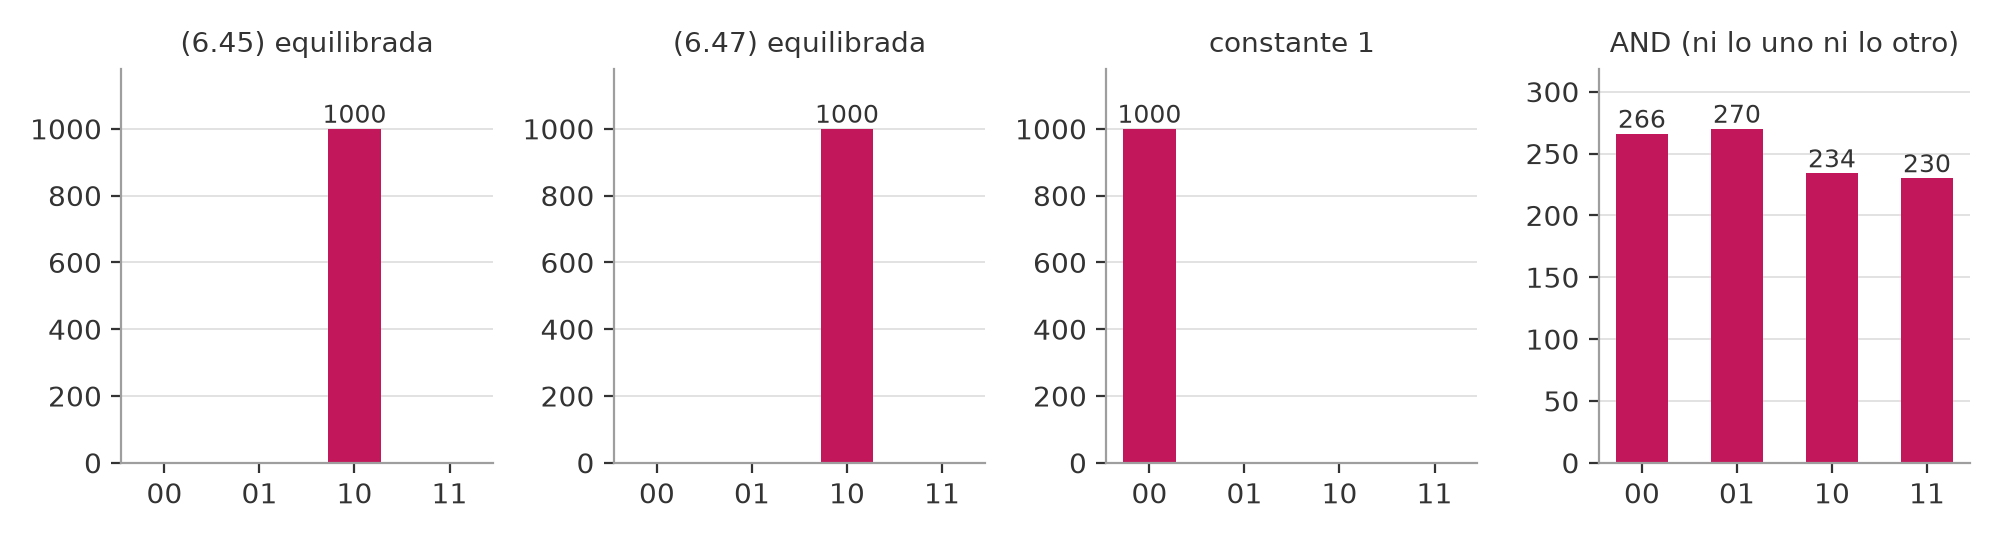
\includegraphics[width=\textwidth]{dj_histogramas.png}

\small Las dos funciones equilibradas nunca dan $\texttt{00}$ (ambas dan $\texttt{10}$, como en el ejemplo completo); la constante da siempre $\texttt{00}$; el AND, que incumple la promesa, da los cuatro resultados con frecuencias próximas a $\frac14 = 250$.
\end{cajafigura}

\noindent Las probabilidades exactas, calculadas con el método \texttt{probabilities\_dict} de \texttt{Statevector}, son $1$ para $\texttt{10}$ en las dos equilibradas, $1$ para $\texttt{00}$ en la constante y $0{,}25$ para cada resultado con el AND. También se comprueba que el estado final de \Yan{6.45} es exactamente $\ket{-}\otimes(-\ket{10})$:
\begin{codigo}
esperado = Statevector(np.kron(np.array([1, -1]) / sqrt(2), -np.eye(4)[2]))
print(Statevector.from_label("000").evolve(qc).equiv(esperado))    # True
\end{codigo}

\subsection{Experimento 3: una función equilibrada de 3 bits al azar}

\noindent Elegimos al azar una función equilibrada de $3$ bits (una permutación aleatoria de cuatro ceros y cuatro unos). Resultó ser
\[ f = (\texttt{000}\mapsto0,\; \texttt{001}\mapsto1,\; \texttt{010}\mapsto1,\; \texttt{011}\mapsto0,\; \texttt{100}\mapsto1,\; \texttt{101}\mapsto1,\; \texttt{110}\mapsto0,\; \texttt{111}\mapsto0). \]
Con $1000$ disparos se obtuvo \texttt{\{'011': 237, '010': 239, '110': 253, '111': 271\}}: nunca $\texttt{000}$, como predice el teorema. La constante $0$ dio \texttt{\{'000': 1000\}}.

\cleardoublepage
\section{Resumen: un ejemplo guiado}

\noindent Seguimos la función equilibrada de \Yan{6.45}: $f(\texttt{00}) = f(\texttt{01}) = 1$, $f(\texttt{10}) = f(\texttt{11}) = 0$.

\pasoguiado{Paso 1. El problema}
{$f:\bits{2}\to\{0,1\}$, con la promesa de que es constante o equilibrada. De las $16$ funciones de $2$ bits, $2$ son constantes y $6$ equilibradas.}
{\textbf{Problema de Deutsch--Jozsa} (con promesa). Funciones equilibradas: $\binom{2^n}{2^{n-1}}$.}

\pasoguiado{Paso 2. Clásicamente}
{Consultamos $f(\texttt{10}) = 0$ y $f(\texttt{11}) = 0$: todavía puede ser la constante $0$. Hace falta una tercera consulta: $2^{n-1}+1 = 3$.}
{\textbf{Cota clásica determinista:} $2^{n-1}+1$ consultas (argumento del adversario). Con azar y un error pequeño bastan unas pocas.}

\pasoguiado{Paso 3. El oráculo}
{$U_f$ intercambia $\ket{000}\leftrightarrow\ket{100}$ y $\ket{001}\leftrightarrow\ket{101}$ (las entradas con $f = 1$) y deja fijos los otros cuatro.}
{$U_f\ket{y}\ket{\bx} = \ket{y\oplus f(\bx)}\ket{\bx}$: permutación, involución, unitaria. En Qiskit, $\bx$ arriba ($\mathsf{q}_0, \mathsf{q}_1$) e $y$ abajo ($\mathsf{q}_2$).}

\pasoguiado{Paso 4. Superposición uniforme}
{$\ket{\varphi_1} = \ket{-}\otimes\tfrac12(\ket{00}+\ket{01}+\ket{10}+\ket{11})$.}
{$H^{\otimes n}\ket{\bcero} = 2^{-n/2}\sum_{\bx}\ket{\bx}$: la primera columna de $H^{\otimes n}$ es toda de unos.}

\pasoguiado{Paso 5. Una consulta}
{$\ket{\varphi_2} = \ket{-}\otimes\tfrac12(-\ket{00}-\ket{01}+\ket{10}+\ket{11})$.}
{\textbf{Retroceso de fase} en todas las componentes a la vez: los signos son $(-1)^{f(\bx)}$.}

\pasoguiado{Paso 6. La fórmula de $H^{\otimes n}$}
{Fila $\texttt{10}$ de $2H^{\otimes2}$: $(1, 1, -1, -1)$, pues $\texttt{00}\cdot\texttt{10} = \texttt{01}\cdot\texttt{10} = 0$ y $\texttt{10}\cdot\texttt{10} = \texttt{11}\cdot\texttt{10} = 1$.}
{$(H^{\otimes n})_{\bz\bx} = 2^{-n/2}(-1)^{\bx\cdot\bz}$, con el \textbf{producto binario} $\bx\cdot\bz$ (paridad de los unos comunes). Se demuestra por inducción.}

\pasoguiado{Paso 7. Interferencia}
{$a_{\texttt{00}} = \tfrac14(-1-1+1+1) = 0$, \quad $a_{\texttt{10}} = \tfrac14(-1-1-1-1) = -1$, \quad $a_{\texttt{01}} = a_{\texttt{11}} = 0$.}
{\textbf{Lema de la suma de signos:} $\sum_{\bx}(-1)^{\bx\cdot\bz} = 0$ si $\bz\neq\bcero$. La amplitud de $\bcero$ es la media de los signos: $\frac{N_0 - N_1}{2^n}$.}

\pasoguiado{Paso 8. Medir}
{Sale $\texttt{10}$ con certeza (Qiskit: \texttt{\{'10': 1000\}}). No es $\texttt{00}$: $f$ es equilibrada.}
{\textbf{Constante} $\iff$ se mide $\bcero$ con probabilidad $1$; \textbf{equilibrada} $\iff$ probabilidad $0$. Una consulta frente a $2^{n-1}+1$.}

\pasoguiado{Paso 9. Si incumplen la promesa}
{AND: $\Pr(\texttt{00}) = \big(\tfrac{3-1}{4}\big)^2 = \tfrac14$.}
{Sin la promesa el algoritmo no decide nada: $\Pr(\bcero) = \big(\frac{N_0-N_1}{2^n}\big)^2$ está estrictamente entre $0$ y $1$.}

\begin{center}
\small\renewcommand{\arraystretch}{1.15}
\begin{tabular}{c|l|l}
\textbf{Paso} & \textbf{Qué hicimos} & \textbf{Concepto} \\ \hline
1 & ¿Constante o equilibrada? & Problema con promesa; contar funciones \\
2 & Consultas clásicas & Cota $2^{n-1}+1$ (adversario) \\
3 & $U_f$ de 3 qubits & Oráculo de $n$ qubits; orden de Qiskit \\
4 & $H^{\otimes2}\ket{00}$ & Superposición uniforme \\
5 & Aplicar $U_f$ & Retroceso de fase en paralelo \\
6 & Fila de $H^{\otimes2}$ & Fórmula de $H^{\otimes n}$, producto binario \\
7 & Amplitudes de $\ket{\varphi_3}$ & Interferencia, suma de signos \\
8 & Medir $\texttt{10}$ & Una consulta, sin error \\
9 & AND & El papel de la promesa
\end{tabular}
\end{center}

% =====================================================================
\chapter{El algoritmo de periodicidad de Simon}

\noindent El algoritmo de Simon \cite{simon1997} busca un \textbf{patrón oculto} en una función: una cadena $\bc$ tal que $f$ toma el mismo valor en $\bx$ y en $\bx\oplus\bc$. Es el primer algoritmo de este cuaderno que \textbf{combina} una parte cuántica, que se repite varias veces y da resultados aleatorios, con una parte \textbf{clásica}, que resuelve un sistema de ecuaciones lineales sobre el cuerpo de dos elementos. Su ventaja es exponencial incluso frente a algoritmos clásicos aleatorios, y su estructura (encontrar un período con la transformada de Hadamard o de Fourier) es la que después usa Shor. Corresponde a la sección 6.3 de Yanofsky.

\cleardoublepage
\section{El problema y la solución clásica}

\begin{teoria}{El problema de Simon}
Se da $f:\bits{n}\to\bits{n}$ como caja negra, con la promesa de que existe una cadena $\bc\in\bits{n}$ tal que, para todas $\bx, \by\in\bits{n}$,
\[ f(\bx) = f(\by) \iff \by = \bx \text{ o } \by = \bx\oplus\bc. \]
La cadena $\bc$ se llama \textbf{período} de $f$. Hay que encontrar $\bc$.
\end{teoria}

\begin{aclaracion}{Nota Aclaratoria: el enunciado del libro}
Yanofsky escribe la condición como ``$f(\bx) = f(\by)$ si y solo si $\bx = \by\oplus\bc$'' \Yan{6.82}. Tomada al pie de la letra, con $\bx = \by$ y $\bc\neq\bcero$ diría que $f(\bx)\neq f(\bx)$, lo cual es absurdo; la lectura correcta es la de arriba, que incluye el caso trivial $\by = \bx$. Para $\bc = \bcero$ las dos lecturas coinciden.
\end{aclaracion}

\begin{teoria}{Proposición: forma de las funciones de Simon}
Si $\bc = \bcero$, $f$ es inyectiva (y, por tanto, biyectiva). Si $\bc\neq\bcero$, $f$ es \textbf{dos a uno}: cada valor de la imagen tiene exactamente dos preimágenes, de la forma $\{\bx, \bx\oplus\bc\}$, y la imagen tiene $2^{n-1}$ elementos.
\end{teoria}

\begin{demo}
Si $\bc = \bcero$, la promesa dice que $f(\bx) = f(\by)$ solo si $\by = \bx$: $f$ es inyectiva, y una aplicación inyectiva de un conjunto finito en sí mismo es biyectiva. Si $\bc\neq\bcero$, para cada $\bx$ las cadenas $\bx$ y $\bx\oplus\bc$ son distintas, tienen la misma imagen, y ninguna otra cadena tiene esa imagen. Las parejas $\{\bx, \bx\oplus\bc\}$ forman una partición de $\bits{n}$ (la relación ``$\by = \bx$ o $\by = \bx\oplus\bc$'' es de equivalencia, porque $(\bx\oplus\bc)\oplus\bc = \bx$), con $2^n/2 = 2^{n-1}$ clases, y $f$ envía clases distintas a valores distintos. \hfill$\square$
\end{demo}

\begin{ejemplo}{Ejemplo 6.3.1 (Yanofsky) y Ejercicio 6.3.1}
\textbf{Con $\bc = \texttt{101}$} ($n = 3$): las parejas $\{\bx, \bx\oplus\texttt{101}\}$ son
\[ \{\texttt{000}, \texttt{101}\}, \quad \{\texttt{001}, \texttt{100}\}, \quad \{\texttt{010}, \texttt{111}\}, \quad \{\texttt{011}, \texttt{110}\}, \]
y la promesa exige $f(\texttt{000}) = f(\texttt{101})$, $f(\texttt{001}) = f(\texttt{100})$, $f(\texttt{010}) = f(\texttt{111})$ y $f(\texttt{011}) = f(\texttt{110})$, con cuatro valores distintos. (El libro lista las ocho igualdades, pero cada una aparece dos veces.)

\textbf{Con $\bc = \texttt{011}$} (Ejercicio 6.3.1): $\texttt{000}\oplus\texttt{011} = \texttt{011}$, $\texttt{001}\oplus\texttt{011} = \texttt{010}$, $\texttt{100}\oplus\texttt{011} = \texttt{111}$ y $\texttt{101}\oplus\texttt{011} = \texttt{110}$, así que
\[ f(\texttt{000}) = f(\texttt{011}), \quad f(\texttt{001}) = f(\texttt{010}), \quad f(\texttt{100}) = f(\texttt{111}), \quad f(\texttt{101}) = f(\texttt{110}), \]
y los cuatro valores tienen que ser distintos entre sí.
\end{ejemplo}

\begin{teoria}{Proposición: solución clásica}
Clásicamente, $\bc$ se encuentra en cuanto se observa una \textbf{colisión}, dos entradas distintas $\bx_1\neq\bx_2$ con $f(\bx_1) = f(\bx_2)$: entonces $\bc = \bx_1\oplus\bx_2$ \Yan{6.85}. Consultando $2^{n-1}+1$ entradas distintas se garantiza encontrar una colisión si $\bc\neq\bcero$, y si no aparece ninguna se concluye que $\bc = \bcero$.
\end{teoria}

\begin{demo}
Si $f(\bx_1) = f(\bx_2)$ con $\bx_1\neq\bx_2$, la promesa da $\bx_2 = \bx_1\oplus\bc$; aplicando $\oplus\,\bx_1$ a los dos lados, $\bx_1\oplus\bx_2 = \bc$ (porque $\bx_1\oplus\bx_1 = \bcero$). Si $\bc\neq\bcero$, la imagen de $f$ tiene $2^{n-1}$ elementos; entre $2^{n-1}+1$ valores de $f$ hay dos iguales por el principio del palomar. Si no hay colisión entre $2^{n-1}+1$ entradas, $\bc\neq\bcero$ es imposible. \hfill$\square$
\end{demo}

\begin{aclaracion}{Nota Aclaratoria: ¿y con un algoritmo aleatorio?}
Consultando entradas al azar se encuentra una colisión mucho antes, por la \textbf{paradoja del cumpleaños}: con unas $2^{n/2}$ consultas la probabilidad de colisión ya es apreciable. Simon demostró que ningún algoritmo clásico, ni siquiera aleatorio, puede hacerlo esencialmente mejor: necesita del orden de $2^{n/2}$ consultas \cite{simon1997}. Como el algoritmo cuántico usa del orden de $n$, la ventaja es exponencial también frente a los algoritmos aleatorios, a diferencia de Deutsch--Jozsa.
\end{aclaracion}

\cleardoublepage
\section{El algoritmo cuántico}

\subsection{El circuito}

\noindent El oráculo tiene ahora un registro de salida de $n$ qubits y hace el XOR bit a bit \Yan{6.83}:
\[ U_f\big(\ket{\bw}\ket{\bx}\big) = \ket{\bw\oplus f(\bx)}\ket{\bx}, \qquad \bx,\bw\in\bits{n}. \]
Como en los capítulos anteriores, es una permutación y su propia inversa. En Qiskit, $\bx$ ocupa $\mathsf{q}_0,\dots,\mathsf{q}_{n-1}$ (arriba) y $\bw$ ocupa $\mathsf{q}_n,\dots,\mathsf{q}_{2n-1}$ (abajo). La parte cuántica del algoritmo es \Yan{6.86}
\begin{center}
\begin{quantikz}
\lstick{$\ket{\bcero}$ \;($\bx$)} & \qwbundle{n} \slice{$\ket{\varphi_0}$} & \gate{H^{\otimes n}} \slice{$\ket{\varphi_1}$} & \gate[2]{U_f} \slice{$\ket{\varphi_2}$} & \gate{H^{\otimes n}} \slice{$\ket{\varphi_3}$} & \meter{} & \setwiretype{c} \\
\lstick{$\ket{\bcero}$ \;($\bw$)} & \qwbundle{n} & & & & &
\end{quantikz}
\end{center}
es decir, $\ket{\varphi_3} = (I\otimes H^{\otimes n})\,U_f\,(I\otimes H^{\otimes n})\,\ket{\bcero}\ket{\bcero}$ (el libro: $(H^{\otimes n}\otimes I)\,U_f\,(H^{\otimes n}\otimes I)\ket{\bcero,\bcero}$, \Yan{6.87}). Obsérvese que esta vez el registro de salida empieza en $\ket{\bcero}$, no en $\ket{-}$: aquí no se usa el retroceso de fase, sino el entrelazamiento entre los dos registros.

\begin{teoria}{Teorema: distribución de los resultados}
Al medir el registro de arriba de $\ket{\varphi_3}$ se obtiene una cadena $\bz$ con probabilidad
\[ \Pr(\bz) = \begin{cases} \dfrac{1}{2^{n-1}} & \text{si } \bz\cdot\bc = 0, \\[2mm] 0 & \text{si } \bz\cdot\bc = 1, \end{cases} \qquad\text{cuando } \bc\neq\bcero, \]
y $\Pr(\bz) = 2^{-n}$ para todo $\bz$ cuando $\bc = \bcero$. Es decir: \textbf{cada ejecución devuelve una cadena uniformemente al azar entre las que cumplen $\bz\cdot\bc = 0$}.
\end{teoria}

\begin{demo}
\textit{Los estados.} Como en Deutsch--Jozsa,
\[ \ket{\varphi_1} = \frac{1}{\sqrt{2^n}}\sum_{\bx}\ket{\bcero}\ket{\bx}, \qquad \ket{\varphi_2} = \frac{1}{\sqrt{2^n}}\sum_{\bx}\ket{f(\bx)}\ket{\bx} \;\;\Yan{6.90}, \]
\[ \ket{\varphi_3} = \frac{1}{2^n}\sum_{\bx}\sum_{\bz}(-1)^{\bx\cdot\bz}\,\ket{f(\bx)}\ket{\bz} \;\;\Yan{6.91}. \]

\textit{Caso $\bc\neq\bcero$.} Agrupamos los sumandos por el valor $\bw = f(\bx)$. Por la proposición anterior, cada $\bw$ de la imagen tiene exactamente dos preimágenes, $\bx_{\bw}$ y $\bx_{\bw}\oplus\bc$, así que el coeficiente de $\ket{\bw}\ket{\bz}$ es
\[ \frac{1}{2^n}\Big((-1)^{\bx_{\bw}\cdot\bz} + (-1)^{(\bx_{\bw}\oplus\bc)\cdot\bz}\Big) = \frac{(-1)^{\bx_{\bw}\cdot\bz}}{2^n}\Big(1 + (-1)^{\bc\cdot\bz}\Big) \;\;\Yan{6.93}, \]
usando $(\bx_{\bw}\oplus\bc)\cdot\bz = \bx_{\bw}\cdot\bz\oplus\bc\cdot\bz$ y $(-1)^{a\oplus b} = (-1)^a(-1)^b$. Si $\bc\cdot\bz = 1$, el paréntesis vale $0$: \textbf{las dos contribuciones interfieren destructivamente}. Si $\bc\cdot\bz = 0$, el coeficiente vale $\pm 2/2^n$. La probabilidad de medir $\bz$ arriba es la suma de los cuadrados de los coeficientes de $\ket{\bw}\ket{\bz}$ sobre todos los $\bw$; si $\bc\cdot\bz = 0$ hay $2^{n-1}$ valores $\bw$ en la imagen, y
\[ \Pr(\bz) = 2^{n-1}\cdot\Big(\frac{2}{2^n}\Big)^2 = \frac{2^{n-1}\cdot4}{4^n} = \frac{1}{2^{n-1}}. \]

\textit{Comprobación de que suman $1$.} Por el lema de la suma de signos, el número de cadenas con $\bz\cdot\bc = 0$ es $\sum_{\bz}\frac{1+(-1)^{\bz\cdot\bc}}{2} = \frac{2^n + 0}{2} = 2^{n-1}$, y $2^{n-1}\cdot2^{-(n-1)} = 1$.

\textit{Caso $\bc = \bcero$.} Ahora $f$ es inyectiva, los kets $\ket{f(\bx)}\ket{\bz}$ son todos distintos y cada uno tiene coeficiente $\pm2^{-n}$. Para cada $\bz$ hay $2^n$ de ellos, luego $\Pr(\bz) = 2^n\cdot4^{-n} = 2^{-n}$. \hfill$\square$
\end{demo}

\begin{aclaracion}{Nota Aclaratoria: la intuición}
Si se midiera primero el registro de abajo (lo que no cambia la distribución del de arriba, porque las operaciones posteriores solo actúan arriba) y saliera $\bw$, el registro de arriba quedaría en $\frac{1}{\sqrt2}(\ket{\bx_{\bw}} + \ket{\bx_{\bw}\oplus\bc})$: una superposición de las dos únicas entradas con ese valor, que ``contiene'' $\bc$ en la diferencia. Pero medir este estado daría $\bx_{\bw}$ o $\bx_{\bw}\oplus\bc$ al azar, sin revelar $\bc$. La $H^{\otimes n}$ final transforma ese ``desplazamiento por $\bc$'' en una \textbf{restricción sobre el resultado}, $\bz\cdot\bc = 0$, que es la misma para todos los $\bw$. Es el análogo binario de un hecho de la transformada de Fourier: una función periódica tiene la transformada concentrada en las frecuencias ``ortogonales'' al período.
\end{aclaracion}

\begin{ejemplo}{Ejemplo completo: la función \Yan{6.94}, con $\bc = \texttt{101}$}
La función es
\[
\begin{array}{c|cccccccc}
\bx & \texttt{000} & \texttt{001} & \texttt{010} & \texttt{011} & \texttt{100} & \texttt{101} & \texttt{110} & \texttt{111} \\ \hline
f(\bx) & \texttt{100} & \texttt{001} & \texttt{101} & \texttt{111} & \texttt{001} & \texttt{100} & \texttt{111} & \texttt{101}
\end{array}
\]
Las parejas con el mismo valor son $\{\texttt{000},\texttt{101}\}\mapsto\texttt{100}$, $\{\texttt{001},\texttt{100}\}\mapsto\texttt{001}$, $\{\texttt{010},\texttt{111}\}\mapsto\texttt{101}$ y $\{\texttt{011},\texttt{110}\}\mapsto\texttt{111}$: en todas, $\bx\oplus\bx' = \texttt{101}$.

\textit{Estados.} $\ket{\varphi_1} = \frac{1}{\sqrt8}\sum_{\bx}\ket{\texttt{000}}\ket{\bx}$ y $\ket{\varphi_2} = \frac{1}{\sqrt8}\big(\ket{\texttt{100}}\ket{\texttt{000}} + \ket{\texttt{001}}\ket{\texttt{001}} + \ket{\texttt{101}}\ket{\texttt{010}} + \cdots + \ket{\texttt{101}}\ket{\texttt{111}}\big)$.

\textit{Un coeficiente a mano.} El coeficiente de $\ket{\texttt{101}}\ket{\texttt{010}}$ en $\ket{\varphi_3}$ (valor $\bw = \texttt{101}$, resultado $\bz = \texttt{010}$) recibe las contribuciones de $\bx = \texttt{010}$ y $\bx = \texttt{111}$:
\[ \tfrac18\big((-1)^{\texttt{010}\cdot\texttt{010}} + (-1)^{\texttt{111}\cdot\texttt{010}}\big) = \tfrac18\big((-1)^1 + (-1)^1\big) = -\tfrac14. \]
El de $\ket{\texttt{101}}\ket{\texttt{001}}$: $\tfrac18\big((-1)^{\texttt{010}\cdot\texttt{001}} + (-1)^{\texttt{111}\cdot\texttt{001}}\big) = \tfrac18(1 - 1) = 0$, y en efecto $\texttt{001}\cdot\texttt{101} = 1$.

\textit{Resultado.} Haciendo las $64$ cuentas (Yanofsky las escribe todas en las páginas 191--192) sobreviven solo los $\bz$ con $\bz\cdot\texttt{101} = 0$:
\begin{align*}
\ket{\varphi_3} = \tfrac14\Big[ &\big(\ket{\texttt{100}} + \ket{\texttt{001}} + \ket{\texttt{101}} + \ket{\texttt{111}}\big)\ket{\texttt{000}} \\ + &\big(\ket{\texttt{100}} + \ket{\texttt{001}} - \ket{\texttt{101}} - \ket{\texttt{111}}\big)\ket{\texttt{010}} \\
+ &\big(\ket{\texttt{100}} - \ket{\texttt{001}} + \ket{\texttt{101}} - \ket{\texttt{111}}\big)\ket{\texttt{101}} \\ + &\big(\ket{\texttt{100}} - \ket{\texttt{001}} - \ket{\texttt{101}} + \ket{\texttt{111}}\big)\ket{\texttt{111}} \Big].
\end{align*}
Cada uno de los cuatro resultados $\texttt{000}, \texttt{010}, \texttt{101}, \texttt{111}$ sale con probabilidad $4\cdot\frac{1}{16} = \frac14 = 2^{-(3-1)}$, como predice el teorema. (Es la última expresión de la página 192 del libro, con los registros en el orden de Qiskit.)

\textit{Encontrar $\bc$.} Escribimos $\bc = c_2c_1c_0$ ($c_0$ es el bit de la derecha). Las ecuaciones $\bz\cdot\bc = 0$ son
\[ \texttt{000}\cdot\bc = 0 \;\text{(no dice nada)}, \qquad \texttt{010}\cdot\bc = c_1 = 0, \]
\[ \texttt{101}\cdot\bc = c_2\oplus c_0 = 0, \qquad \texttt{111}\cdot\bc = c_2\oplus c_1\oplus c_0 = 0. \]
De la segunda, $c_1 = 0$; de la tercera, $c_2 = c_0$. Las soluciones son $\texttt{000}$ y $\texttt{101}$, y como $f$ no es inyectiva (por ejemplo, $f(\texttt{000}) = f(\texttt{101})$), $\bc = \texttt{101}$.
\end{ejemplo}

\begin{ejercicio}{Ejercicio 6.3.2 (Yanofsky): la función \Yan{6.99}}
La función es
\[
\begin{array}{c|cccccccc}
\bx & \texttt{000} & \texttt{001} & \texttt{010} & \texttt{011} & \texttt{100} & \texttt{101} & \texttt{110} & \texttt{111} \\ \hline
f(\bx) & \texttt{000} & \texttt{100} & \texttt{100} & \texttt{000} & \texttt{010} & \texttt{110} & \texttt{110} & \texttt{010}
\end{array}
\]
Parejas: $\{\texttt{000},\texttt{011}\}\mapsto\texttt{000}$, $\{\texttt{001},\texttt{010}\}\mapsto\texttt{100}$, $\{\texttt{100},\texttt{111}\}\mapsto\texttt{010}$, $\{\texttt{101},\texttt{110}\}\mapsto\texttt{110}$; en todas la diferencia es $\texttt{011}$, así que $\bc = \texttt{011}$. Las cadenas con $\bz\cdot\texttt{011} = 0$ son $\texttt{000}, \texttt{011}, \texttt{100}, \texttt{111}$, y
\begin{align*}
\ket{\varphi_3} = \tfrac14\Big[ &\big(\ket{\texttt{000}} + \ket{\texttt{100}} + \ket{\texttt{010}} + \ket{\texttt{110}}\big)\ket{\texttt{000}} \\ + &\big(\ket{\texttt{000}} + \ket{\texttt{100}} - \ket{\texttt{010}} - \ket{\texttt{110}}\big)\ket{\texttt{011}} \\
+ &\big(\ket{\texttt{000}} - \ket{\texttt{100}} + \ket{\texttt{010}} - \ket{\texttt{110}}\big)\ket{\texttt{100}} \\ + &\big(\ket{\texttt{000}} - \ket{\texttt{100}} - \ket{\texttt{010}} + \ket{\texttt{110}}\big)\ket{\texttt{111}} \Big].
\end{align*}
Por ejemplo, el coeficiente de $\ket{\texttt{010}}\ket{\texttt{011}}$ viene de $\bx = \texttt{100}$ y $\texttt{111}$: $\frac18\big((-1)^{0} + (-1)^{0}\big) = \frac14$; el de $\ket{\texttt{100}}\ket{\texttt{011}}$ viene de $\texttt{001}$ y $\texttt{010}$: $\frac18\big((-1)^1 + (-1)^1\big) = -\frac14$. Con los resultados $\texttt{100}$ y $\texttt{011}$: $c_2 = 0$ y $c_1\oplus c_0 = 0$, luego $\bc\in\{\texttt{000}, \texttt{011}\}$ y $\bc = \texttt{011}$.
\end{ejercicio}

\subsection{La parte clásica: ecuaciones lineales sobre $\F$}

\noindent Cada ejecución da una ecuación lineal $\bz\cdot\bc = 0$ para las $n$ incógnitas $c_{n-1},\dots,c_0\in\{0,1\}$. Es un sistema lineal homogéneo sobre el cuerpo $\F = \{0,1\}$ (con $\oplus$ como suma), y se resuelve por \textbf{eliminación gaussiana} exactamente como sobre $\mathbb{R}$: ``sumar una ecuación a otra'' es hacer el XOR de las cadenas, y no hace falta dividir porque el único coeficiente no nulo es $1$.

\begin{teoria}{Proposición: cuándo el sistema determina $\bc$}
Sea $\bc\neq\bcero$ y sean $\bz_1,\dots,\bz_k$ cadenas con $\bz_i\cdot\bc = 0$. Si el subespacio $W$ que generan tiene dimensión $n-1$, el conjunto de soluciones de $\{\bz_i\cdot\mathbf{u} = 0\}_{i=1}^k$ es exactamente $\{\bcero, \bc\}$.
\end{teoria}

\begin{demo}
Sea $Z$ la matriz $k\times n$ sobre $\F$ cuyas filas son las $\bz_i$. Las soluciones son el núcleo de $Z$, y el rango de $Z$ es $\dim W = n-1$. Por el teorema del rango (válido sobre cualquier cuerpo), el núcleo tiene dimensión $n - (n-1) = 1$, así que tiene $2^1 = 2$ elementos. Como $\bcero$ y $\bc$ son soluciones y son distintos, son todas. \hfill$\square$
\end{demo}

\begin{ejemplo}{Ejemplo 6.3.2 (Yanofsky): eliminación con $n = 7$}
Siete ejecuciones dan las ecuaciones $\bz_i\cdot\bc = 0$ con
\[ \text{(i) } \texttt{1010110}, \; \text{(ii) } \texttt{0010001}, \; \text{(iii) } \texttt{1100101}, \; \text{(iv) } \texttt{0011011}, \]
\[ \text{(v) } \texttt{0101001}, \; \text{(vi) } \texttt{0011010}, \; \text{(vii) } \texttt{0110111}. \]
Los pasos del libro (comprobados uno a uno con código) son:
\begin{enumerate}
\item (iii) $\oplus$= (i): (iii) pasa a $\texttt{0110011}$ (se limpia la primera columna).
\item (v) $\oplus$= (iii) y (vii) $\oplus$= (iii): (v) $= \texttt{0011010}$, (vii) $= \texttt{0000100}$.
\item (i), (iii), (iv), (v), (vi) $\oplus$= (ii): $\texttt{1000111}$, $\texttt{0100010}$, $\texttt{0001010}$, $\texttt{0001011}$, $\texttt{0001011}$.
\item (v), (vi) $\oplus$= (iv) y (i) $\oplus$= (vii): (v) $=$ (vi) $= \texttt{0000001}$, (i) $= \texttt{1000011}$.
\item (i), (ii), (vi) $\oplus$= (v): (i) $= \texttt{1000010}$, (ii) $= \texttt{0010000}$, (vi) $= \texttt{0000000}$.
\end{enumerate}
Numerando los bits de $\bc$ de izquierda a derecha como hace el libro, $\bc = d_1d_2\cdots d_7$, queda
\[ d_1\oplus d_6 = 0, \quad d_3 = 0, \quad d_2\oplus d_6 = 0, \quad d_4\oplus d_6 = 0, \quad d_7 = 0, \quad d_5 = 0. \]
Hay $6$ ecuaciones independientes (la (vi) se anuló: era combinación de las demás), el rango es $6 = n-1$ y las soluciones son $d_6 = 0$ (todo ceros) o $d_6 = 1$, que da $\bc = \texttt{1101010}$.
\end{ejemplo}

\begin{aclaracion}{Una corrección al libro: el Ejercicio 6.3.3 no tiene solución única}
El Ejercicio 6.3.3 pide resolver
\[ \texttt{11110000},\; \texttt{01101001},\; \texttt{10010110},\; \texttt{00111100}, \]
\[ \texttt{11111111},\; \texttt{11000011},\; \texttt{10001110},\; \texttt{01110001}, \]
y da como pista $\bc = \texttt{10011001}$. Esa cadena cumple las ocho ecuaciones, pero \textbf{no es la única}: el sistema tiene rango $5$, no $7$, y por el teorema del rango sus soluciones forman un subespacio de dimensión $8 - 5 = 3$, con $8$ elementos. Las siete soluciones no nulas son
\[ \texttt{10011001},\; \texttt{01011010},\; \texttt{11000011},\; \texttt{00111100},\; \texttt{10100101},\; \texttt{01100110},\; \texttt{11111111}. \]
El motivo es que tres de las ecuaciones son combinaciones de otras:
\[ \text{(v)} = \text{(ii)}\oplus\text{(iii)}, \qquad \text{(vi)} = \text{(iv)}\oplus\text{(v)}, \qquad \text{(viii)} = \text{(v)}\oplus\text{(vii)}, \]
por ejemplo $\texttt{01101001}\oplus\texttt{10010110} = \texttt{11111111}$. Quedan $8 - 3 = 5$ ecuaciones independientes. En una ejecución real del algoritmo de Simon se seguiría ejecutando el circuito hasta que el rango llegara a $n - 1 = 7$; con estas ocho ecuaciones todavía no se puede afirmar cuál es $\bc$.
\end{aclaracion}

\subsection{¿Cuántas ejecuciones hacen falta?}

\noindent Yanofsky afirma que el período se encuentra ``con $n$ evaluaciones de la función'' \Yan{p.~195}. No es exactamente así: los resultados son aleatorios y pueden repetirse o ser combinaciones de los anteriores (en el Experimento 4 una ejecución da tres veces seguidas el mismo resultado). Lo correcto es que el número \textbf{medio} de ejecuciones es menor que $n+1$, y se demuestra a continuación.

\begin{teoria}{Teorema: número de ejecuciones del algoritmo de Simon}
Sea $\bc\neq\bcero$ y sea $V = \{\bz : \bz\cdot\bc = 0\}$, un subespacio de dimensión $n-1$. Si se ejecuta la parte cuántica hasta que los resultados generen $V$:
\begin{enumerate}
\item la probabilidad de que basten exactamente $n-1$ ejecuciones es $\prod_{j=1}^{n-1}\big(1 - 2^{-j}\big) > \frac14$;
\item el número medio de ejecuciones es $\displaystyle\sum_{j=1}^{n-1}\frac{1}{1-2^{-j}} < n + 1$.
\end{enumerate}
\end{teoria}

\begin{demo}
Por el teorema anterior, cada ejecución devuelve un elemento de $V$ uniformemente al azar, independientemente de las demás. Supongamos que los resultados obtenidos hasta ahora generan un subespacio $W\subseteq V$ de dimensión $r < n-1$. La siguiente ejecución aumenta la dimensión si y solo si su resultado no está en $W$, lo que ocurre con probabilidad
\[ p_r = 1 - \frac{|W|}{|V|} = 1 - \frac{2^r}{2^{n-1}} = 1 - 2^{-(n-1-r)}. \]

\textit{Apartado 1.} Bastan $n-1$ ejecuciones si y solo si cada una aumenta la dimensión, con $r = 0, 1, \dots, n-2$; la probabilidad es $\prod_{r=0}^{n-2}p_r = \prod_{j=1}^{n-1}(1-2^{-j})$ (cambiando $j = n-1-r$). Para acotarla usamos que $(1-a)(1-b)\ge 1-a-b$ si $a, b\ge0$, que por inducción da $\prod_k(1-a_k)\ge 1-\sum_k a_k$:
\[ \prod_{j=1}^{n-1}(1-2^{-j}) = \tfrac12\prod_{j=2}^{n-1}(1-2^{-j}) \ge \tfrac12\Big(1 - \sum_{j=2}^{\infty}2^{-j}\Big) = \tfrac12\cdot\tfrac12 = \tfrac14, \]
con desigualdad estricta para $n\ge3$ (para $n = 2$ vale $\frac12$).

\textit{Apartado 2.} Mientras la dimensión es $r$, el número de ejecuciones hasta aumentarla es una variable geométrica de parámetro $p_r$, cuya media es $1/p_r$. Por la linealidad de la esperanza, el número medio total es
\[ \sum_{r=0}^{n-2}\frac{1}{p_r} = \sum_{j=1}^{n-1}\frac{1}{1-2^{-j}} = \sum_{j=1}^{n-1}\Big(1 + \frac{1}{2^j-1}\Big) = (n-1) + \sum_{j=1}^{n-1}\frac{1}{2^j-1}. \]
Como $2^j - 1\ge 2^{j-1}$, la última suma es menor que $\sum_{j\ge1}2^{-(j-1)} = 2$, y el total es menor que $n+1$. (Numéricamente, $\sum_{j\ge1}\frac{1}{2^j-1}\approx1{,}607$.) \hfill$\square$
\end{demo}

\begin{ejemplo}{Ejemplo: los números para $n = 3$}
$V$ tiene $4$ elementos. Con $r = 0$ (aún no hay nada útil), cualquier resultado distinto de $\texttt{000}$ sirve: $p_0 = \frac34$. Con $r = 1$ ($W$ tiene $2$ elementos), sirven $2$ de los $4$: $p_1 = \frac12$. La probabilidad de terminar en $2$ ejecuciones es $\frac34\cdot\frac12 = \frac38 = 0{,}375$, y la media es $\frac43 + 2 = \frac{10}{3}\approx3{,}33$. Una simulación de $20\,000$ repeticiones da una media de $3{,}34$.
\end{ejemplo}

\begin{aclaracion}{Nota Aclaratoria: el caso $\bc = \bcero$ y el algoritmo completo}
Si no se sabe de antemano que $\bc\neq\bcero$, se procede así: se ejecuta el circuito hasta que el rango de los resultados sea al menos $n-1$. Si llega a $n$, el sistema solo tiene la solución $\bcero$ y $\bc = \bcero$. Si es $n-1$, hay una única solución no nula $\bc'$, y con dos consultas clásicas se comprueba si $f(\bcero) = f(\bc')$: si es así, $\bc = \bc'$; si no, $\bc = \bcero$. En total se usan $O(n)$ consultas y $O(n^3)$ operaciones clásicas (la eliminación gaussiana).
\end{aclaracion}

\cleardoublepage
\section{Implementación en Qiskit}

\subsection{Experimento 4: el algoritmo de Simon con las funciones del libro}

\noindent Usamos la función \texttt{oraculo(f, n, m)} del capítulo anterior con $m = n = 3$, y una función auxiliar que convierte la tabla de valores del libro en una función de enteros:
\begin{codigo}
def de_tabla(tabla):
    """Convierte un diccionario {'01': '1', ...} en una función entera."""
    return lambda x: int(tabla[format(x, "0%db" % len(next(iter(tabla))))], 2)

def simon(f, n):
    qc = QuantumCircuit(2 * n, n)
    qc.h(range(n))
    qc.barrier()
    qc.append(oraculo(f, n, n), range(2 * n))
    qc.barrier()
    qc.h(range(n))
    qc.measure(range(n), range(n))
    return qc

f_694 = {"000": "100", "001": "001", "010": "101", "011": "111",
         "100": "001", "101": "100", "110": "111", "111": "101"}
\end{codigo}

\begin{cajafigura}
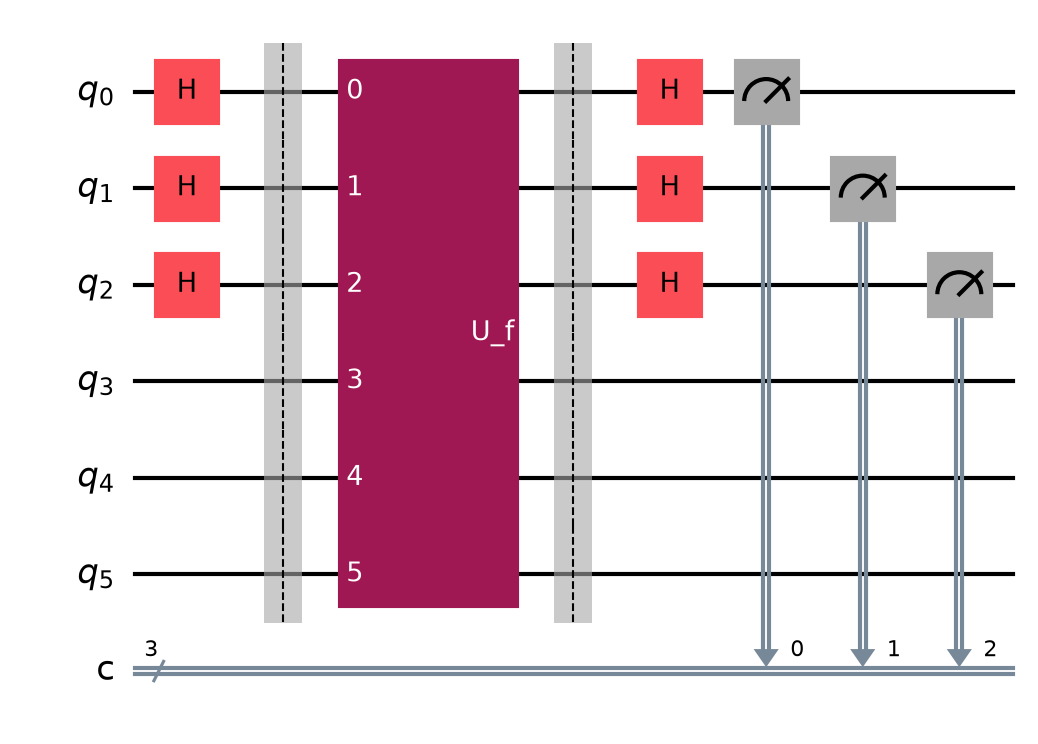
\includegraphics[width=0.5\textwidth]{simon_circuito.png}

\small El circuito de Simon con $n = 3$: el registro $\bx$ son $\mathsf{q}_0,\mathsf{q}_1,\mathsf{q}_2$ (arriba) y el registro de salida $\mathsf{q}_3,\mathsf{q}_4,\mathsf{q}_5$ (abajo); solo se mide el de arriba.
\end{cajafigura}

\noindent Con $1000$ disparos:
\begin{codigo}[language={}]
Simon (6.94) {'111': 246, '101': 238, '000': 250, '010': 266}
Simon (6.99) {'011': 257, '111': 264, '100': 245, '000': 234}
\end{codigo}

\begin{cajafigura}
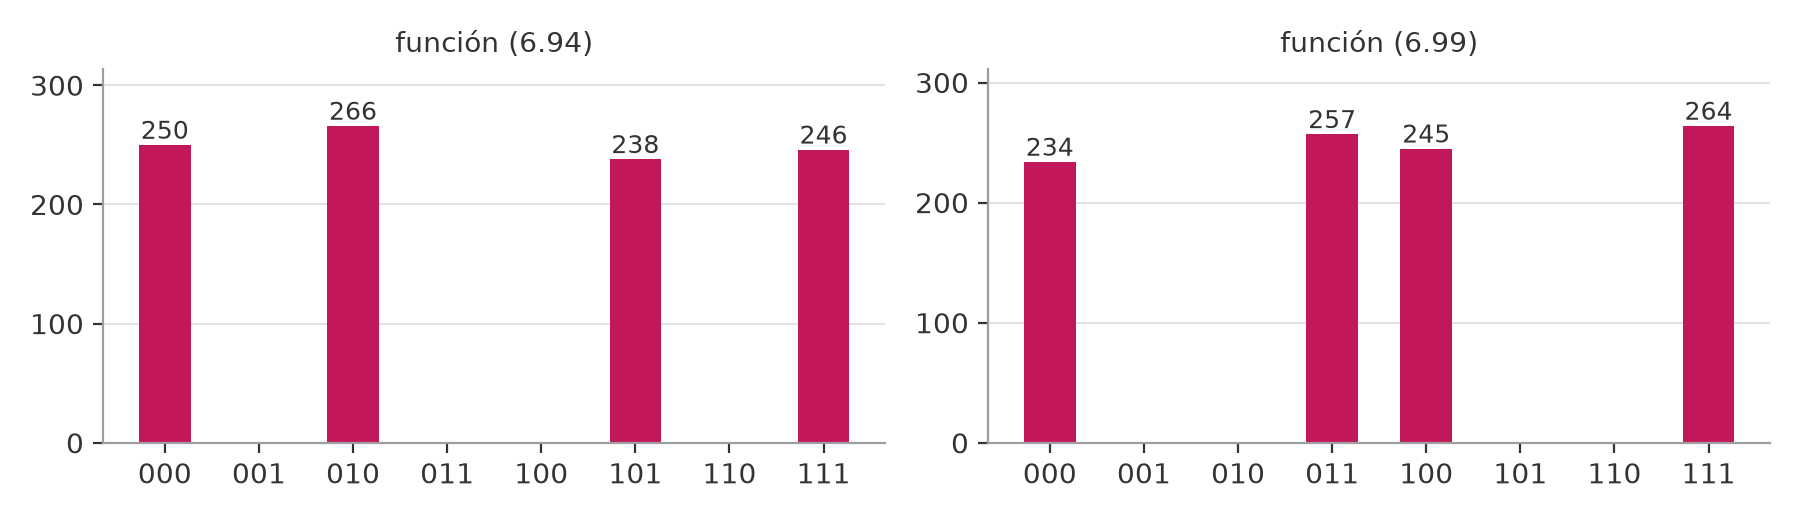
\includegraphics[width=\textwidth]{simon_histogramas.png}

\small Solo aparecen las cuatro cadenas con $\bz\cdot\bc = 0$ ($\bc = \texttt{101}$ a la izquierda y $\bc = \texttt{011}$ a la derecha), cada una con frecuencia próxima a $\frac14$.
\end{cajafigura}

\subsection{Experimento 5: el algoritmo completo, ejecución a ejecución}

\noindent Para resolver el sistema programamos la eliminación gaussiana sobre $\F$, guardando cada cadena como un entero para que ``sumar ecuaciones'' sea el XOR \texttt{\^{}}:
\begin{codigo}
def resolver_F2(ecuaciones, n):
    """Rango y soluciones c != 0 de z.c = 0 (mod 2), por eliminación gaussiana."""
    filas, pivotes = [], []
    for z in ecuaciones:
        v = int(z, 2)
        for fila, p in zip(filas, pivotes):   # reducir con las filas ya guardadas
            if v >> p & 1:
                v ^= fila
        if v:                                 # nueva fila independiente
            p = v.bit_length() - 1
            for i in range(len(filas)):       # forma escalonada reducida
                if filas[i] >> p & 1:
                    filas[i] ^= v
            filas.append(v)
            pivotes.append(p)
    ...   # se recorren los valores de las variables libres (ver el programa)
    return len(filas), soluciones
\end{codigo}
\noindent Ejecutamos el circuito de disparo en disparo (\texttt{get\_bitstrings()} da el resultado de cada disparo en orden) hasta que el rango es $n-1 = 2$:
\begin{codigo}[language={}]
(6.94): ejecuciones ['000', '111', '101'] -> rango 2 -> c = ['101']
(6.99): ejecuciones ['111', '111', '111', '100'] -> rango 2 -> c = ['011']
\end{codigo}
\noindent En el primer caso el resultado $\texttt{000}$ no aporta nada y hacen falta $3$ ejecuciones; en el segundo, $\texttt{111}$ sale tres veces seguidas y hacen falta $4$. Las dos cifras están cerca de la media teórica $\frac{10}{3}$.

\noindent Por último, el mismo programa resuelve los sistemas del libro:
\begin{codigo}[language={}]
Ejemplo 6.3.2:   (6, ['1101010'])
Ejercicio 6.3.3: (5, ['10011001', '01011010', '11000011', '00111100',
                      '10100101', '01100110', '11111111'])
\end{codigo}
\noindent El Ejemplo 6.3.2 tiene rango $6 = n-1$ y solución única; el Ejercicio 6.3.3 tiene rango $5$ y siete soluciones no nulas, como se explicó en la corrección.

\cleardoublepage
\section{Resumen: un ejemplo guiado}

\noindent Seguimos la función de \Yan{6.94}, con período $\bc = \texttt{101}$.

\pasoguiado{Paso 1. El problema}
{$f(\texttt{000}) = f(\texttt{101}) = \texttt{100}$, \; $f(\texttt{001}) = f(\texttt{100}) = \texttt{001}$, \; $f(\texttt{010}) = f(\texttt{111}) = \texttt{101}$, \; $f(\texttt{011}) = f(\texttt{110}) = \texttt{111}$.}
{\textbf{Problema de Simon:} $f(\bx) = f(\by)\iff\by\in\{\bx, \bx\oplus\bc\}$. Si $\bc\neq\bcero$, $f$ es \textbf{dos a uno}.}

\pasoguiado{Paso 2. Clásicamente}
{Si encontramos $f(\texttt{000}) = f(\texttt{101})$, entonces $\bc = \texttt{000}\oplus\texttt{101} = \texttt{101}$. Para garantizarlo hacen falta $2^{n-1}+1 = 5$ consultas.}
{\textbf{Colisión} $\Rightarrow$ período. Clásicamente: $2^{n-1}+1$ (determinista), del orden de $2^{n/2}$ (aleatorio).}

\pasoguiado{Paso 3. Superposición y consulta}
{$\ket{\varphi_2} = \frac{1}{\sqrt8}\sum_{\bx}\ket{f(\bx)}\ket{\bx}$: cada valor $\bw$ aparece junto a sus dos preimágenes.}
{El oráculo de $n+n$ qubits \textbf{entrelaza} la entrada con la salida. Aquí no hay retroceso de fase: la salida empieza en $\ket{\bcero}$.}

\pasoguiado{Paso 4. Interferencia}
{Coeficiente de $\ket{\texttt{101}}\ket{\texttt{001}}$: $\frac18\big((-1)^{\texttt{010}\cdot\texttt{001}} + (-1)^{\texttt{111}\cdot\texttt{001}}\big) = \frac18(1-1) = 0$.}
{Las preimágenes $\bx$ y $\bx\oplus\bc$ contribuyen con $(-1)^{\bx\cdot\bz}(1 + (-1)^{\bc\cdot\bz})$: se cancelan si $\bz\cdot\bc = 1$.}

\pasoguiado{Paso 5. Medir}
{Se obtiene $\texttt{000}, \texttt{010}, \texttt{101}$ o $\texttt{111}$, cada uno con probabilidad $\frac14$. Qiskit: \texttt{\{'111': 246, '101': 238, '000': 250, '010': 266\}}.}
{Cada ejecución da un $\bz$ \textbf{uniforme} en $\{\bz:\bz\cdot\bc = 0\}$, un subespacio de dimensión $n-1$.}

\pasoguiado{Paso 6. Ecuaciones}
{$\texttt{010}\cdot\bc = c_1 = 0$, \quad $\texttt{101}\cdot\bc = c_2\oplus c_0 = 0$ \;$\Rightarrow$\; $\bc\in\{\texttt{000}, \texttt{101}\}$ \;$\Rightarrow$\; $\bc = \texttt{101}$.}
{\textbf{Eliminación gaussiana sobre $\F$}. Con rango $n-1$ las soluciones son exactamente $\{\bcero,\bc\}$ (teorema del rango).}

\pasoguiado{Paso 7. Cuántas veces}
{Ejecuciones de Qiskit: $\texttt{000}$ (inútil), $\texttt{111}$, $\texttt{101}$: rango $2$ tras $3$ ejecuciones. Media teórica para $n = 3$: $\frac{10}{3}$.}
{Número medio de ejecuciones $< n+1$; probabilidad de terminar en $n-1$ ejecuciones $> \frac14$. (Yanofsky dice ``$n$ evaluaciones'': es la idea, no un número exacto.)}

\begin{center}
\small\renewcommand{\arraystretch}{1.15}
\begin{tabular}{c|l|l}
\textbf{Paso} & \textbf{Qué hicimos} & \textbf{Concepto} \\ \hline
1 & Tabla de $f$ & Período $\bc$; funciones dos a uno \\
2 & Buscar una colisión & Cota clásica; paradoja del cumpleaños \\
3 & $U_f$ sobre la superposición & Entrelazamiento entrada--salida \\
4 & Un coeficiente a mano & Interferencia destructiva si $\bz\cdot\bc = 1$ \\
5 & Medir & $\bz$ uniforme en $\bc^{\perp}$ \\
6 & Resolver & Álgebra lineal sobre $\F$ \\
7 & Contar ejecuciones & Media $< n+1$
\end{tabular}
\end{center}

% =====================================================================
\chapter{El algoritmo de búsqueda de Grover}

\noindent El algoritmo de Grover \cite{grover1996} busca un elemento marcado entre $N = 2^n$ posibles con unas $\frac{\pi}{4}\sqrt N$ consultas, frente a las del orden de $N$ que necesita cualquier algoritmo clásico. La ventaja es ``solo'' cuadrática, pero el problema es mucho más general que los de los capítulos anteriores (no hay ninguna promesa sobre la estructura de $f$) y se sabe que ningún algoritmo cuántico puede hacerlo mejor \cite{bennett1997}. Combina dos reflexiones: la \textbf{inversión de fase} y la \textbf{inversión respecto de la media}. Yanofsky deja sin demostrar por qué hay que repetirlas unas $\sqrt N$ veces; aquí se demuestra, con la interpretación geométrica que el libro recomienda. Corresponde a la sección 6.4 de Yanofsky.

\cleardoublepage
\section{El problema y la solución clásica}

\begin{teoria}{El problema de búsqueda}
Se da $f:\bits{n}\to\{0,1\}$ como caja negra, con la promesa de que hay \textbf{exactamente una} cadena $\bx_0$ con $f(\bx_0) = 1$ \Yan{6.100}:
\[ f(\bx) = \begin{cases} 1 & \text{si } \bx = \bx_0, \\ 0 & \text{si } \bx\neq\bx_0. \end{cases} \]
Hay que encontrar $\bx_0$. Escribimos $N = 2^n$ para el número de candidatos.
\end{teoria}

\noindent Es la versión abstracta de buscar en una lista desordenada: $f(\bx)$ responde a la pregunta ``¿es $\bx$ el elemento buscado?''.

\begin{teoria}{Proposición: cota clásica}
Un algoritmo clásico determinista necesita $N-1$ consultas en el peor caso. Uno aleatorio que acierte con probabilidad al menos $\frac12$ necesita del orden de $N$ consultas (al menos $N/2 - 1$).
\end{teoria}

\begin{demo}
\textit{Determinista.} Con $N-1$ consultas basta: si todas dan $0$, el elemento es el que falta. Si se hacen $k\le N-2$ consultas, un adversario responde $0$ a todas; quedan al menos dos candidatos no consultados, ambos compatibles con todo lo observado, y el algoritmo falla en uno de ellos.

\textit{Aleatorio.} Supongamos que $\bx_0$ se elige uniformemente al azar. Mientras no se encuentra $\bx_0$, todas las respuestas son $0$, así que el algoritmo no aprende nada salvo qué cadenas descartar. La probabilidad de que $\bx_0$ esté entre las $k$ cadenas consultadas es $k/N$; si no está, el algoritmo tiene que adivinar entre las $N-k$ restantes y acierta con probabilidad $1/(N-k)$. En total,
\[ \Pr(\text{éxito})\le\frac{k}{N} + \frac{N-k}{N}\cdot\frac{1}{N-k} = \frac{k+1}{N}, \]
y para que valga al menos $\frac12$ hace falta $k\ge\frac N2 - 1$. (Si funciona con probabilidad $\ge\frac12$ para todo $\bx_0$, también la tiene en media sobre $\bx_0$ elegido al azar.) \hfill$\square$
\end{demo}

\noindent En media, un algoritmo que consulta en orden aleatorio encuentra $\bx_0$ tras unas $N/2$ consultas \Yan{p.~196}. Grover lo hace con unas $\frac{\pi}{4}\sqrt N$: para $N = 10^6$, unas $785$ consultas en lugar de medio millón.

\cleardoublepage
\section{El algoritmo cuántico}

\subsection{El oráculo y un primer intento}

\noindent El oráculo es el mismo de Deutsch--Jozsa, $U_f\ket{y}\ket{\bx} = \ket{y\oplus f(\bx)}\ket{\bx}$: solo cambia $y$ cuando $\bx = \bx_0$.

\begin{ejercicio}{Ejercicio 6.4.1 (Yanofsky): los oráculos de búsqueda para $n = 2$}
En el orden de Qiskit (base $\ket{y\,x_1x_0}$), el oráculo que marca $\bx_0$ intercambia $\ket{0}\ket{\bx_0}\leftrightarrow\ket{1}\ket{\bx_0}$ y deja fijos los otros seis vectores. Es decir, en la matriz $8\times8$ (identidad salvo un intercambio de dos columnas):
\[
\renewcommand{\arraystretch}{1.2}
\begin{array}{c|c}
\bx_0 & \text{vectores que se intercambian} \\ \hline
\texttt{00} & \ket{000}\leftrightarrow\ket{100} \\
\texttt{01} & \ket{001}\leftrightarrow\ket{101} \\
\texttt{10} & \ket{010}\leftrightarrow\ket{110} \quad\text{(el de \Yan{6.101})} \\
\texttt{11} & \ket{011}\leftrightarrow\ket{111}
\end{array}
\]
En \Yan{6.101}, con el orden de Yanofsky, el intercambio es $\ket{10,0}\leftrightarrow\ket{10,1}$: los mismos dos estados. Cada uno de estos oráculos es una puerta $X$ sobre $y$ \textbf{controlada} por los dos qubits de $\bx$, con los controles ``en $0$'' donde $\bx_0$ tiene un $0$ (Experimento 7).
\end{ejercicio}

\noindent \textbf{Primer intento} \Yan{6.102}: poner $\bx$ en superposición uniforme, $y$ en $\ket{0}$, y consultar. Se obtiene $\ket{\varphi_2} = \frac{1}{\sqrt N}\sum_{\bx}\ket{f(\bx)}\ket{\bx}$. Al medir, $y = 1$ con probabilidad $\frac1N$ (solo la componente $\bx_0$ tiene $y = 1$), y en ese caso el registro de arriba da $\bx_0$. Pero eso es tan improbable como acertar al azar. Hace falta amplificar la amplitud de $\bx_0$.

\subsection{Primer ingrediente: la inversión de fase}

\noindent Con $y$ en $\ket{-}$, el lema del retroceso de fase da $U_f\big(\ket{-}\ket{\bx}\big) = (-1)^{f(\bx)}\ket{-}\ket{\bx}$ \Yan{6.113}. Sobre el registro de arriba, el efecto es el operador diagonal
\[ Z_f = \sum_{\bx}(-1)^{f(\bx)}\ket{\bx}\bra{\bx} = I - 2\ket{\bx_0}\bra{\bx_0}, \]
que \textbf{cambia el signo de la amplitud de $\bx_0$} y deja las demás igual. Es la \textbf{inversión de fase}.

\begin{ejemplo}{Ejemplo: inversión de fase con $n = 2$}
Con $\bx_0 = \texttt{10}$ y el estado uniforme $\frac12(1,1,1,1)^T$ (componentes $\texttt{00}, \texttt{01}, \texttt{10}, \texttt{11}$), la inversión de fase da $\frac12(1,1,-1,1)^T$ \Yan{p.~198}. Medir no distingue nada: $|\pm\frac12|^2 = \frac14$ para las cuatro cadenas. La fase separa $\bx_0$ de las demás, pero no de forma observable.
\end{ejemplo}

\begin{aclaracion}{Nota Aclaratoria: el qubit auxiliar se prepara una sola vez}
Yanofsky escribe la inversión de fase como $U_f(I\otimes H)$ aplicada a $\ket{\bx,1}$ \Yan{6.109}, e incluye esa $H$ dentro del bucle del algoritmo \Yan{6.134}. Leído al pie de la letra, aplicar $H$ en cada iteración devolvería $y$ de $\ket{-}$ a $\ket{1}$ y estropearía el algoritmo. Lo correcto es preparar $\ket{-} = H\ket{1}$ \textbf{una vez} al principio: por el lema del retroceso de fase, $\ket{-}$ es un autovector de $U_f$ y \textbf{sigue siendo $\ket{-}$ tras cada consulta}, así que cada aplicación posterior de $U_f$ actúa como $Z_f$ sobre el registro de arriba.
\end{aclaracion}

\subsection{Segundo ingrediente: la inversión respecto de la media}

\noindent Dada una lista de números $v_1,\dots,v_N$ con media $a = \frac1N\sum_i v_i$, \textbf{invertir respecto de la media} es reflejar cada número al otro lado de $a$, a la misma distancia \Yan{6.114, 6.115}:
\[ v_i' = a + (a - v_i) = 2a - v_i. \]

\begin{ejemplo}{Ejemplo: la lista $53, 38, 17, 23, 79$ (figuras 6.1 y 6.2 del libro)}
La media es $a = \frac{210}{5} = 42$. Entonces $v_1' = 84 - 53 = 31$, $v_2' = 84 - 38 = 46$, $v_3' = 67$, $v_4' = 61$, $v_5' = 5$. La media de la lista nueva sigue siendo $\frac{31+46+67+61+5}{5} = 42$: los números que estaban $11$ por encima quedan $11$ por debajo, y al revés.
\begin{cajafigura}
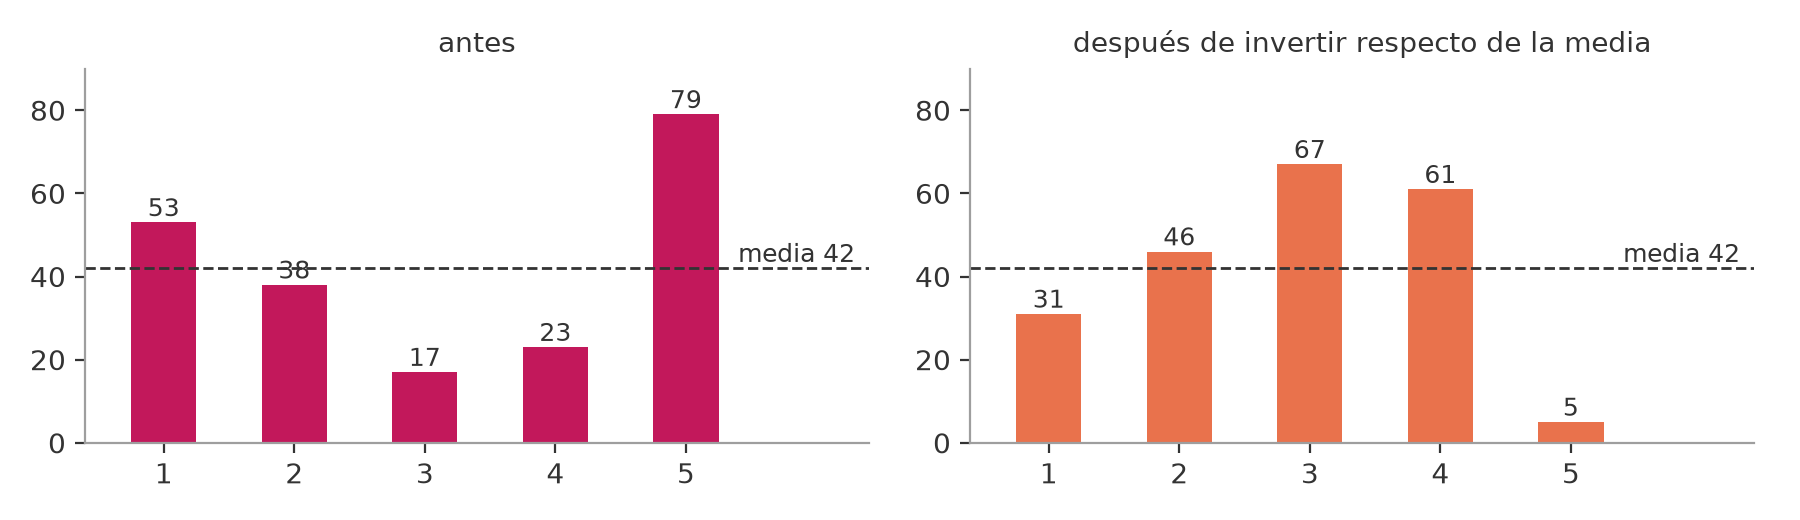
\includegraphics[width=0.95\textwidth]{grover_media.png}
\end{cajafigura}
\end{ejemplo}

\begin{ejercicio}{Ejercicio 6.4.2 (Yanofsky)}
Para $5, 38, 62, 58, 21, 35$: la media es $\frac{219}{6} = 36{,}5$ y $2a = 73$, así que la lista invertida es
\[ 73-5 = 68, \quad 73-38 = 35, \quad 73-62 = 11, \quad 73-58 = 15, \quad 73-21 = 52, \quad 73-35 = 38, \]
de media $\frac{219}{6} = 36{,}5$ otra vez.
\end{ejercicio}

\noindent En forma matricial, la media se obtiene con la matriz $A$ de tamaño $N\times N$ con todas las entradas iguales a $\frac1N$ \Yan{6.116, 6.122}: $AV$ es el vector con todas las componentes iguales a la media de $V$. La inversión es entonces $V' = 2AV - V = (-I + 2A)V$ \Yan{6.118}. Para la lista anterior, $(-I+2A)(53, 38, 17, 23, 79)^T = (31, 46, 67, 61, 5)^T$ \Yan{6.121}, comprobado con \texttt{numpy}.

\begin{teoria}{Proposición: la inversión respecto de la media es una reflexión unitaria}
Sea $N = 2^n$, $A$ la matriz $N\times N$ con todas las entradas $\frac1N$, $D = -I + 2A$ y $\ket{s} = H^{\otimes n}\ket{\bcero} = \frac{1}{\sqrt N}\sum_{\bx}\ket{\bx}$. Entonces:
\begin{enumerate}
\item $A^2 = A$ \;(Ejercicio 6.4.3), y de hecho $A = \ket{s}\bra{s}$;
\item $D$ es unitaria y $D^2 = I$;
\item $D = 2\ket{s}\bra{s} - I = H^{\otimes n}\big(2\ket{\bcero}\bra{\bcero} - I\big)H^{\otimes n}$.
\end{enumerate}
Geométricamente, $D$ es la \textbf{reflexión respecto de la recta generada por $\ket{s}$}: deja fijo $\ket{s}$ y cambia el signo de todo vector ortogonal a $\ket{s}$.
\end{teoria}

\begin{demo}
\textit{1.} La entrada $(\bx,\by)$ de $\ket{s}\bra{s}$ es $\braket{\bx}{s}\braket{s}{\by} = \frac{1}{\sqrt N}\cdot\frac{1}{\sqrt N} = \frac1N$, así que $A = \ket{s}\bra{s}$. Como $\braket{s}{s} = N\cdot\frac1N = 1$, $A^2 = \ket{s}\braket{s}{s}\bra{s} = \ket{s}\bra{s} = A$. (Directamente: la entrada $(\bx,\by)$ de $A^2$ es $\sum_{\bz}\frac1N\cdot\frac1N = N\cdot\frac{1}{N^2} = \frac1N$.)

\textit{2.} $D$ es real y simétrica, luego $D^\dagger = D$, y \Yan{6.124}
\[ D^\dagger D = D^2 = (-I+2A)^2 = I - 4A + 4A^2 = I - 4A + 4A = I. \]

\textit{3.} La primera igualdad es $D = -I + 2A$ con $A = \ket{s}\bra{s}$. Para la segunda, como $H^{\otimes n}$ es autoadjunta, $(H^{\otimes n})^2 = I$ y $H^{\otimes n}\ket{\bcero} = \ket{s}$:
\[ H^{\otimes n}\big(2\ket{\bcero}\bra{\bcero} - I\big)H^{\otimes n} = 2\big(H^{\otimes n}\ket{\bcero}\big)\big(H^{\otimes n}\ket{\bcero}\big)^\dagger - (H^{\otimes n})^2 = 2\ket{s}\bra{s} - I. \]

\textit{Reflexión.} $D\ket{s} = 2\ket{s}\braket{s}{s} - \ket{s} = \ket{s}$, y si $\braket{s}{\psi} = 0$, $D\ket{\psi} = -\ket{\psi}$. \hfill$\square$
\end{demo}

\noindent La inversión de fase también es una reflexión: $Z_f = I - 2\ket{\bx_0}\bra{\bx_0}$ deja fijo todo vector ortogonal a $\ket{\bx_0}$ y cambia el signo de $\ket{\bx_0}$. Grover alterna dos reflexiones, y la composición de dos reflexiones es un \textbf{giro}. Esta es la clave de la demostración de la sección siguiente.

\begin{ejemplo}{Ejemplo 6.4.1 (Yanofsky) y Ejercicio 6.4.4: las dos operaciones juntas}
Partimos de $(10, 10, 10, 10, 10)$ y marcamos siempre la cuarta componente (el vector no está normalizado; lo que importa es el mecanismo). Cada fila es una iteración: primero se cambia el signo de la cuarta componente y después se invierte respecto de la media.
\[
\renewcommand{\arraystretch}{1.25}
\begin{array}{c|c|c|c|c}
k & \text{media } a & \text{componentes 1, 2, 3, 5} & \text{componente 4 (marcada)} & \text{diferencia} \\ \hline
1 & 6 & 2 & 22 & 20 \\
2 & -2{,}8 & -7{,}6 & 16{,}4 & 24 \\
3 & -9{,}36 & -11{,}12 & -2{,}32 & 8{,}8
\end{array}
\]
Por ejemplo, en la fila 2 la lista tras la inversión de fase es $(2, 2, 2, -22, 2)$, de media $\frac{8-22}{5} = -2{,}8$. La fila 3 es el Ejercicio 6.4.4: \textbf{el resultado empeora}. La cuarta componente, que llevaba ventaja, queda por debajo de las demás en valor absoluto ($|-2{,}32| < |-11{,}12|$). Es lo que Yanofsky llama ``pasarse de cocción'' (\textit{overcook}). Observemos también que la suma de los cuadrados es $500$ en todas las filas: las dos operaciones conservan la norma, como debe ser para matrices unitarias.
\end{ejemplo}

\subsection{El algoritmo}

\noindent Llamamos \textbf{iteración de Grover} a $G = D\,Z_f$ (primero la inversión de fase, después la inversión respecto de la media).

\begin{teoria}{Algoritmo de Grover (versión corregida del enunciado del libro)}
\begin{enumerate}
\item Preparar el registro de $n$ qubits en $\ket{\bcero}$ y el qubit auxiliar en $\ket{1}$.
\item Aplicar $H^{\otimes n}$ al registro (queda $\ket{s}$) y $H$ al auxiliar (queda $\ket{-}$), \textbf{una sola vez}.
\item Repetir $k = \lfloor\pi/(4\theta)\rfloor$ veces, donde $\theta = \arcsin(1/\sqrt N)$ (para $N$ grande, $k\approx\frac{\pi}{4}\sqrt N$):
\begin{enumerate}
\item[3a.] inversión de fase: aplicar $U_f$ (que actúa como $Z_f$ sobre el registro);
\item[3b.] inversión respecto de la media: aplicar $D = -I + 2A$ al registro.
\end{enumerate}
\item Medir el registro.
\end{enumerate}
\end{teoria}

\begin{center}
\begin{quantikz}
\lstick{$\ket{\bcero}$ \;($\bx$)} & \qwbundle{n} & \gate{H^{\otimes n}} & \gate[2]{U_f}\gategroup[2,steps=2,style={dashed,rounded corners,fill=rosaclaro!20,inner xsep=2pt},background,label style={label position=above,anchor=north,yshift=0.3cm}]{repetir $k$ veces} & \gate{-I+2A} & \meter{} & \setwiretype{c} \\
\lstick{$\ket{1}$ \;($y$)} & & \gate{H} & & & &
\end{quantikz}
\end{center}

\begin{aclaracion}{Una corrección al libro: el número de iteraciones}
Yanofsky dice que hay que repetir el paso 3 ``$\sqrt{2^n}$ veces'' \Yan{p.~202}. El orden de magnitud es correcto, pero \textbf{el número exacto importa}, porque el algoritmo es periódico y pasarse lo estropea:
\begin{itemize}
\item para $n = 3$, $\sqrt8\approx2{,}83$, que redondeado da $3$ iteraciones y una probabilidad de éxito de solo $0{,}330$; con $k = \lfloor\pi/(4\theta)\rfloor = 2$ iteraciones (las que hace el propio ejemplo del libro) es $0{,}945$;
\item para $n = 4$, $\sqrt{16} = 4$ iteraciones dan $0{,}582$, mientras que $k = 3$ da $0{,}961$.
\end{itemize}
El número correcto es aproximadamente $\frac{\pi}{4}\sqrt{2^n}\approx 0{,}785\sqrt{2^n}$, y se demuestra en el teorema siguiente.
\end{aclaracion}

\begin{ejemplo}{Ejemplo 6.4.2 (Yanofsky): $n = 3$, $\bx_0 = \texttt{101}$}
Escribimos las amplitudes del registro (componentes $\texttt{000}$ a $\texttt{111}$; la de $\texttt{101}$ es la sexta).

\textit{Superposición.} $\ket{\varphi_2} = \frac{1}{\sqrt8}(1,1,1,1,1,1,1,1)$ \Yan{6.136}.

\textit{Iteración 1.} Inversión de fase: $\frac{1}{\sqrt8}(1,1,1,1,1,-1,1,1)$. Media: $a = \frac18\cdot\frac{7-1}{\sqrt8} = \frac{3}{4\sqrt8}$ \Yan{6.138}. Inversión: las no marcadas pasan a $2a - \frac{1}{\sqrt8} = \frac{3}{2\sqrt8} - \frac{2}{2\sqrt8} = \frac{1}{2\sqrt8}$, y la marcada a $2a + \frac{1}{\sqrt8} = \frac{5}{2\sqrt8}$ \Yan{6.139--6.141}.

\textit{Iteración 2.} Inversión de fase: la sexta pasa a $-\frac{5}{2\sqrt8}$. Media: $a = \frac18\cdot\frac{7 - 5}{2\sqrt8} = \frac{1}{8\sqrt8}$ \Yan{6.143}. Inversión: no marcadas $\frac{2}{8\sqrt8} - \frac{1}{2\sqrt8} = -\frac{1}{4\sqrt8}$; marcada $\frac{2}{8\sqrt8} + \frac{5}{2\sqrt8} = \frac{11}{4\sqrt8}$ \Yan{6.144--6.146}.

\textit{Medición.} $\Pr(\texttt{101}) = \big(\frac{11}{4\sqrt8}\big)^2 = \frac{121}{128}\approx0{,}9453$ y cada una de las otras siete sale con probabilidad $\frac{1}{128}$ ($7\cdot\frac{1}{128} + \frac{121}{128} = 1$). Los decimales del libro son $\frac{11}{4\sqrt8}\approx0{,}97227$ y $-\frac{1}{4\sqrt8}\approx-0{,}08839$.
\begin{cajafigura}
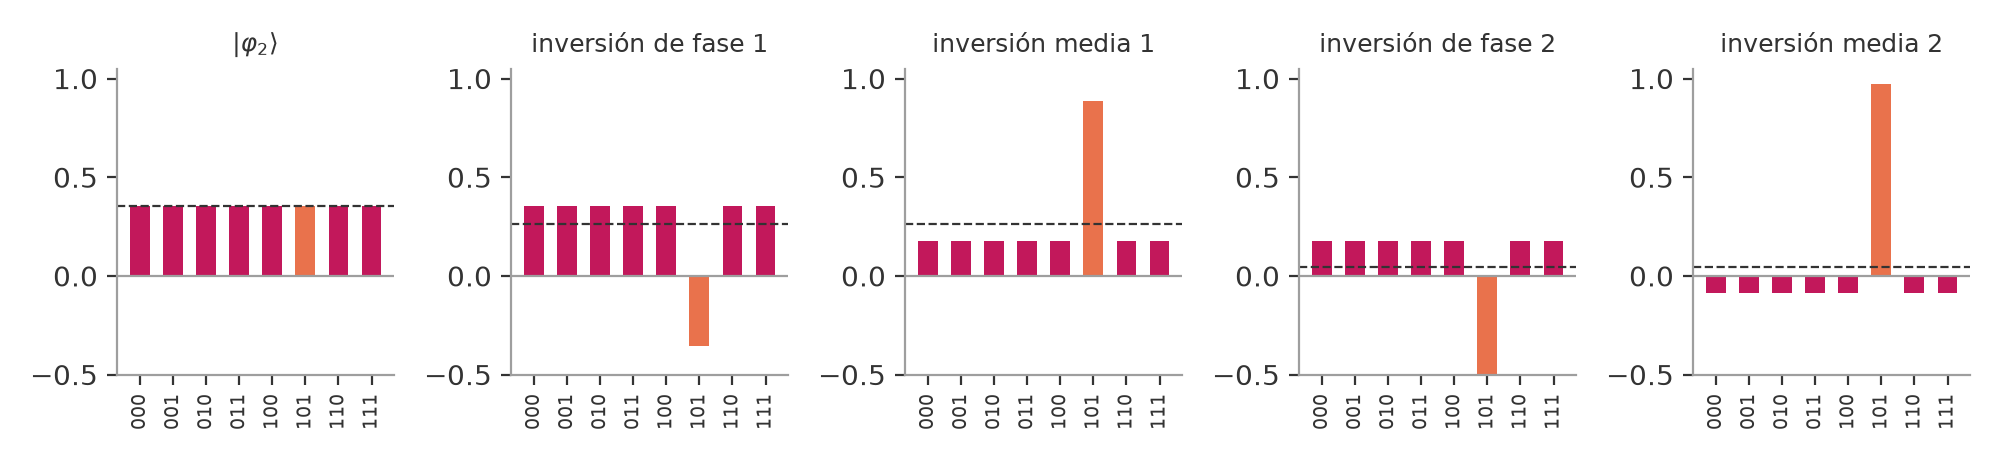
\includegraphics[width=\textwidth]{grover_amplitudes.png}

\small Las amplitudes en cada paso (en salmón, la de $\texttt{101}$; la línea discontinua es la media). Cada inversión de fase baja la marcada por debajo de cero; cada inversión respecto de la media la sube muy por encima.
\end{cajafigura}
\end{ejemplo}

\subsection{Demostración: por qué $\frac{\pi}{4}\sqrt N$ iteraciones}

\noindent Yanofsky afirma que la prueba ``está fuera del alcance del texto'' pero usa ``una geometría muy bonita''. Es esta.

\begin{teoria}{Teorema: el algoritmo de Grover gira el estado}
Sean $\ket{\beta} = \ket{\bx_0}$, $\ket{\alpha} = \frac{1}{\sqrt{N-1}}\sum_{\bx\neq\bx_0}\ket{\bx}$ y $\theta\in(0,\frac{\pi}{2}]$ con $\sin\theta = \frac{1}{\sqrt N}$. Entonces, para todo $k\ge0$,
\[ G^k\ket{s} = \cos\big((2k+1)\theta\big)\ket{\alpha} + \sin\big((2k+1)\theta\big)\ket{\beta}, \]
y la probabilidad de obtener $\bx_0$ tras $k$ iteraciones es $\sin^2\big((2k+1)\theta\big)$.
\end{teoria}

\begin{demo}
\textit{El plano invariante.} $\ket{\alpha}$ y $\ket{\beta}$ son ortonormales (tienen soporte disjunto y norma $1$), y
\[ \ket{s} = \frac{1}{\sqrt N}\sum_{\bx}\ket{\bx} = \sqrt{\frac{N-1}{N}}\,\ket{\alpha} + \frac{1}{\sqrt N}\ket{\beta} = \cos\theta\ket{\alpha} + \sin\theta\ket{\beta}, \]
pues $\cos\theta = \sqrt{1 - 1/N}$. Veamos que $Z_f$ y $D$ envían el plano $P = \mathrm{span}\{\ket{\alpha},\ket{\beta}\}$ a sí mismo y calculemos sus matrices en la base $(\ket{\alpha},\ket{\beta})$.

\textit{Inversión de fase.} $Z_f\ket{\alpha} = \ket{\alpha}$ (no contiene $\bx_0$) y $Z_f\ket{\beta} = -\ket{\beta}$:
$Z_f|_P = \left(\begin{smallmatrix} 1 & 0\\ 0 & -1\end{smallmatrix}\right)$, la reflexión respecto del eje $\ket{\alpha}$.

\textit{Inversión respecto de la media.} $D = 2\ket{s}\bra{s} - I$, y $\ket{s} = (\cos\theta, \sin\theta)^T$ en esta base. Para $\ket{v}\in P$, $D\ket{v} = 2\braket{s}{v}\ket{s} - \ket{v}\in P$, con matriz
\[ D|_P = 2\begin{pmatrix}\cos\theta\\ \sin\theta\end{pmatrix}\begin{pmatrix}\cos\theta & \sin\theta\end{pmatrix} - I = \begin{pmatrix} 2\cos^2\theta - 1 & 2\sin\theta\cos\theta \\ 2\sin\theta\cos\theta & 2\sin^2\theta - 1\end{pmatrix} = \begin{pmatrix}\cos2\theta & \sin2\theta \\ \sin2\theta & -\cos2\theta\end{pmatrix}. \]

\textit{La iteración es un giro.} Multiplicando,
\[ G|_P = D|_P\,Z_f|_P = \begin{pmatrix}\cos2\theta & \sin2\theta \\ \sin2\theta & -\cos2\theta\end{pmatrix}\begin{pmatrix} 1 & 0\\ 0 & -1\end{pmatrix} = \begin{pmatrix}\cos2\theta & -\sin2\theta \\ \sin2\theta & \cos2\theta\end{pmatrix}, \]
que es el \textbf{giro de ángulo $2\theta$}. Por tanto $G^k|_P$ es el giro de ángulo $2k\theta$ (la potencia de un giro es el giro del ángulo multiplicado, por las fórmulas de adición del seno y el coseno, o por inducción), y aplicado a $\ket{s}$, que forma un ángulo $\theta$ con $\ket{\alpha}$, da el vector de ángulo $(2k+1)\theta$:
\[ G^k\ket{s} = \cos\big((2k+1)\theta\big)\ket{\alpha} + \sin\big((2k+1)\theta\big)\ket{\beta}. \]

\textit{Probabilidad.} La amplitud de $\ket{\bx_0} = \ket{\beta}$ es $\sin((2k+1)\theta)$, y el qubit auxiliar está en $\ket{-}$, factorizado. Por la regla de Born, $\Pr(\bx_0) = \sin^2((2k+1)\theta)$. \hfill$\square$
\end{demo}

\begin{center}
\begin{tikzpicture}[scale=3.2, >={Stealth}]
  \def\t{20.7}
  \draw[->, gray] (-0.15,0) -- (1.25,0) node[right, tinta] {$\ket{\alpha}$ (no marcadas)};
  \draw[->, gray] (0,-0.5) -- (0,1.2) node[above, tinta] {$\ket{\beta} = \ket{\bx_0}$};
  \draw[thick, ->, rosa] (0,0) -- ({cos(\t)},{sin(\t)}) node[right] {$\ket{s}$};
  \draw[thick, ->, salmon] (0,0) -- ({cos(\t)},{-sin(\t)}) node[right] {$Z_f\ket{s}$};
  \draw[thick, ->, rosa] (0,0) -- ({cos(3*\t)},{sin(3*\t)}) node[above right] {$G\ket{s}$};
  \draw[thick, ->, rosa] (0,0) -- ({cos(5*\t)},{sin(5*\t)}) node[above] {$G^2\ket{s}$};
  \draw[dashed, gray] (0,0) -- ({1.15*cos(\t)},{1.15*sin(\t)});
  \draw[gray] (0.32,0) arc (0:\t:0.32); \node[tinta, font=\small] at (0.42,0.07) {$\theta$};
  \draw[gray] ({0.22*cos(\t)},{0.22*sin(\t)}) arc (\t:3*\t:0.22); \node[tinta, font=\small] at (0.24,0.28) {$2\theta$};
\end{tikzpicture}
\end{center}
\noindent \textit{Figura:} el caso $N = 8$ ($\theta\approx20{,}7^\circ$). $Z_f$ refleja $\ket{s}$ respecto del eje horizontal; $D$ refleja el resultado respecto de la recta de $\ket{s}$ (discontinua). El efecto neto es un giro de $2\theta$ hacia $\ket{\bx_0}$. Tras dos iteraciones el ángulo es $5\theta\approx103{,}5^\circ$, ya muy cerca de la vertical: $\sin^2(5\theta) = 0{,}945$.

\begin{teoria}{Corolario: número de iteraciones}
Con $k = \lfloor\pi/(4\theta)\rfloor$ iteraciones, la probabilidad de éxito es al menos $1 - \frac1N$, y $k\le\frac{\pi}{4}\sqrt N$.
\end{teoria}

\begin{demo}
De $\frac{\pi}{4\theta} - 1 < k\le\frac{\pi}{4\theta}$ se obtiene, multiplicando por $2\theta$ y sumando $\theta$, $\frac{\pi}{2} - \theta < (2k+1)\theta\le\frac{\pi}{2} + \theta$. Es decir, el ángulo final dista de $\frac{\pi}{2}$ como mucho $\theta$, y como $\sin^2$ es simétrica respecto de $\frac{\pi}{2}$ y creciente en $[0,\frac{\pi}{2}]$,
\[ \sin^2\big((2k+1)\theta\big)\ge\sin^2\big(\tfrac{\pi}{2} - \theta\big) = \cos^2\theta = 1 - \tfrac1N. \]
Además, $\theta\ge\sin\theta = \frac{1}{\sqrt N}$ (pues $\sin t\le t$ para $t\ge0$), luego $k\le\frac{\pi}{4\theta}\le\frac{\pi}{4}\sqrt N$. \hfill$\square$
\end{demo}

\begin{ejemplo}{Ejemplo: los números para $n = 3$ y $n = 4$}
$n = 3$: $\theta = \arcsin(1/\sqrt8)\approx0{,}3614$, $\frac{\pi}{4\theta}\approx2{,}17$, $k = 2$ y $\Pr = \sin^2(5\theta) = \frac{121}{128}\approx0{,}945\ge1 - \frac18$.

$n = 4$: $\theta = \arcsin(\frac14)\approx0{,}2527$, $\frac{\pi}{4\theta}\approx3{,}11$, $k = 3$ y $\Pr = \sin^2(7\theta)\approx0{,}961\ge1 - \frac{1}{16}$.

Con más iteraciones el estado sigue girando y \textbf{se aleja} de $\ket{\bx_0}$: para $n = 3$, $\Pr = 0{,}330$ con $k = 3$ y $0{,}012$ con $k = 4$, y vuelve a acercarse con $k = 6$ ($0{,}9998$). Esto explica el ``exceso de cocción'' del Ejercicio 6.4.4.
\end{ejemplo}

\begin{ejercicio}{Ejercicio 6.4.5 (Yanofsky): $n = 4$, $\bx_0 = \texttt{1101}$}
Hay $16$ amplitudes, todas iguales a $\frac14$ al principio. Por simetría, en cada paso las $15$ no marcadas son iguales entre sí; llamamos $u$ a su valor y $m$ al de la marcada. Cada iteración hace $m\mapsto -m$ y luego, con $a = \frac{15u - m}{16}$, $u\mapsto2a - u$ y $-m\mapsto 2a + m$.
\[
\renewcommand{\arraystretch}{1.35}
\begin{array}{c|c|c|c|c}
k & \text{media } a & u & m & \Pr(\texttt{1101}) = m^2 \\ \hline
0 & - & \frac14 & \frac14 & 0{,}0625 \\
1 & \frac{7}{32} & \frac{3}{16} & \frac{11}{16} & 0{,}4727 \\
2 & \frac{17}{128} & \frac{5}{64} & \frac{61}{64} & 0{,}9084 \\
3 & \frac{7}{512} & -\frac{13}{256} & \frac{251}{256} & \mathbf{0{,}9613} \\
4 & -\frac{223}{2048} & -\frac{171}{1024} & \frac{781}{1024} & 0{,}5817
\end{array}
\]
Por ejemplo, en la iteración 1: $a = \frac{15\cdot\frac14 - \frac14}{16} = \frac{14/4}{16} = \frac{7}{32}$, $u = \frac{7}{16} - \frac14 = \frac{3}{16}$ y $m = \frac{7}{16} + \frac14 = \frac{11}{16}$. Comprobación de la norma en $k = 3$: $15\cdot\frac{169}{65536} + \frac{63001}{65536} = \frac{65536}{65536} = 1$. Lo óptimo son $3$ iteraciones, como da el corolario; con las $4$ que sugiere el libro la probabilidad cae a $0{,}58$. Los valores de $m$ coinciden con $\sin\big((2k+1)\theta\big)$ para $\theta = \arcsin\frac14$.
\end{ejercicio}

\begin{aclaracion}{Nota Aclaratoria: varias soluciones y optimalidad}
\textbf{Varias soluciones.} Si hay $t$ cadenas marcadas \Yan{p.~204}, la misma demostración vale con $\ket{\beta}$ la superposición uniforme de las marcadas, $\ket{\alpha}$ la de las no marcadas y $\sin\theta = \sqrt{t/N}$. El número de iteraciones es $\lfloor\pi/(4\theta)\rfloor\approx\frac{\pi}{4}\sqrt{N/t}$ (el libro da $\sqrt{N/t}$, que es el orden de magnitud). Un caso curioso: si $t = N/4$, $\theta = \frac{\pi}{6}$ y \textbf{una} iteración da probabilidad $\sin^2(\frac{\pi}{2}) = 1$. Si $t$ no se conoce, hay variantes que eligen el número de iteraciones al azar \cite{boyer1998}.

\textbf{Optimalidad.} Bennett, Bernstein, Brassard y Vazirani \cite{bennett1997} demostraron que todo algoritmo cuántico que resuelva el problema de búsqueda necesita del orden de $\sqrt N$ consultas: Grover es óptimo. Por eso la ventaja cuántica en búsqueda no estructurada es cuadrática y no exponencial.
\end{aclaracion}

\begin{tfg}
El ángulo inicial del algoritmo es $\sin^2\theta = |\braket{s}{\bx_0}|^2 = \frac1N = 2^{-n}$: el estado uniforme y un estado de la base son \textbf{casi ortogonales} cuando hay muchos qubits. Es el mismo fenómeno que está detrás de la \textbf{concentración exponencial} de los kernels cuánticos (Thanasilp et al.\ \cite{thanasilp2024exponential}): en un espacio de dimensión $2^n$, dos estados ``típicos'' tienen fidelidad $|\braket{\phi(\mathbf{x})}{\phi(\mathbf{y})}|^2$ del orden de $2^{-n}$, y distinguir valores tan pequeños con disparos requiere del orden de $2^n$ repeticiones. Grover saca partido de amplitudes de tamaño $2^{-n/2}$ amplificándolas coherentemente; un kernel estimado midiendo no puede hacerlo.
\end{tfg}

\cleardoublepage
\section{Implementación en Qiskit}

\subsection{Experimento 6: el oráculo y la difusión con puertas}

\noindent Esta vez construimos las dos reflexiones con puertas, como se haría en un ordenador cuántico real. El oráculo es una $X$ multicontrolada sobre el auxiliar (\texttt{mcx}), con puertas $X$ antes y después sobre los qubits en los que $\bx_0$ tiene un $0$, para que el control se active con $\ket{\bx_0}$ y solo con él:
\begin{codigo}
def oraculo_grover(marcado, n):
    qc = QuantumCircuit(n + 1, name="U_f")
    ceros = [q for q in range(n) if not (marcado >> q) & 1]
    if ceros:
        qc.x(ceros)
    qc.mcx(list(range(n)), n)
    if ceros:
        qc.x(ceros)
    return qc
\end{codigo}
\noindent Para la difusión usamos la proposición: $D = H^{\otimes n}(2\ket{\bcero}\bra{\bcero} - I)H^{\otimes n}$. A su vez, $I - 2\ket{\bcero}\bra{\bcero} = X^{\otimes n}\big(I - 2\ket{1\cdots1}\bra{1\cdots1}\big)X^{\otimes n}$, y $I - 2\ket{1\cdots1}\bra{1\cdots1}$ es la $Z$ multicontrolada, que se obtiene como $H$, $X$ multicontrolada y $H$ sobre el último qubit. Juntando,
\[ H^{\otimes n}X^{\otimes n}\,(\text{MCZ})\,X^{\otimes n}H^{\otimes n} = H^{\otimes n}\big(I - 2\ket{\bcero}\bra{\bcero}\big)H^{\otimes n} = -D. \]
\begin{codigo}
def difusion(n):
    """-(H X MCZ X H) = -I + 2A, salvo el signo global."""
    qc = QuantumCircuit(n, name="-I+2A")
    qc.h(range(n))
    qc.x(range(n))
    qc.h(n - 1)
    qc.mcx(list(range(n - 1)), n - 1)
    qc.h(n - 1)
    qc.x(range(n))
    qc.h(range(n))
    return qc
\end{codigo}
\noindent El circuito implementa $-D$: difiere de $D$ en una \textbf{fase global} $-1$, que no afecta a ninguna probabilidad. Lo comprobamos para $n = 2, 3, 4$:
\begin{codigo}[language={}]
n=2: Operator(difusion) == -(-I+2A): True     oráculo con puertas == U_f: True
n=3: Operator(difusion) == -(-I+2A): True     oráculo con puertas == U_f: True
n=4: Operator(difusion) == -(-I+2A): True     oráculo con puertas == U_f: True
\end{codigo}

\subsection{Experimento 7: el algoritmo completo}

\begin{codigo}
def grover(marcado, n, iteraciones, medir=True):
    qc = QuantumCircuit(n + 1, n)
    qc.x(n)
    qc.h(n)                 # qubit auxiliar en |->, una sola vez
    qc.h(range(n))
    for _ in range(iteraciones):
        qc.barrier()
        qc.compose(oraculo_grover(marcado, n), range(n + 1), inplace=True)
        qc.compose(difusion(n), range(n), inplace=True)
    if medir:
        qc.measure(range(n), range(n))
    return qc
\end{codigo}

\begin{cajafigura}
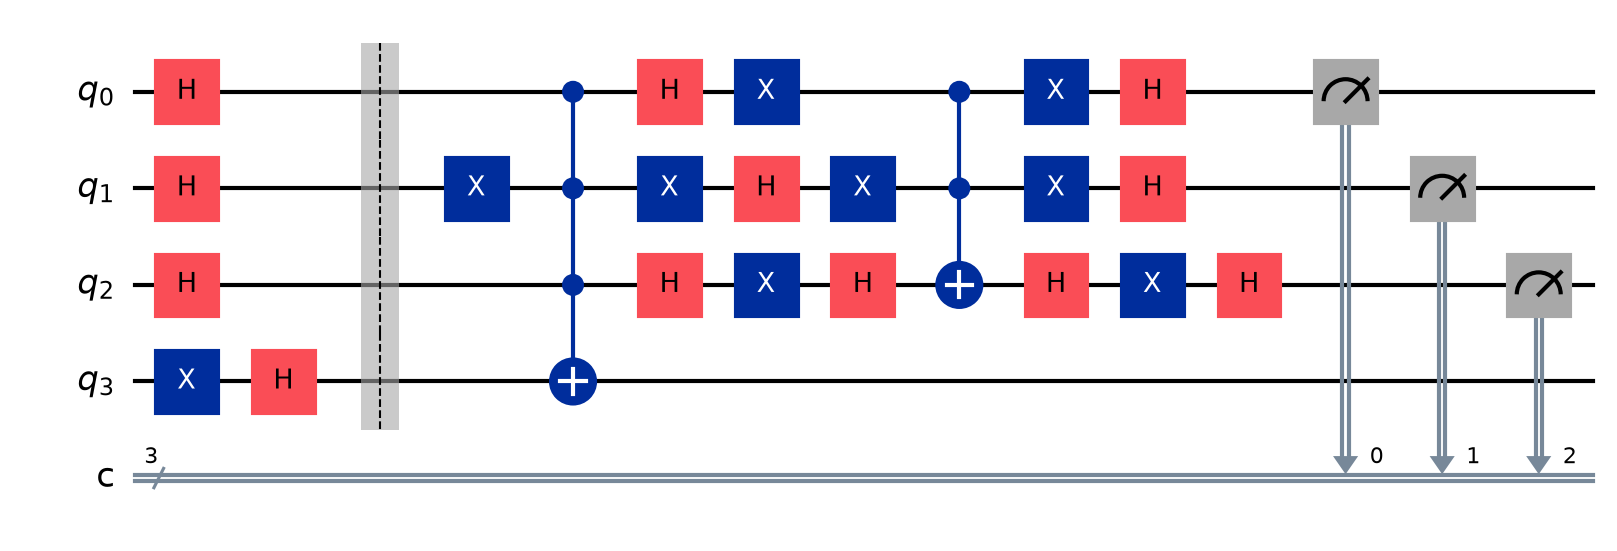
\includegraphics[width=\textwidth]{grover_circuito.png}

\small Una iteración de Grover para $n = 3$ y $\bx_0 = \texttt{101}$. El oráculo es la $X$ con tres controles sobre $\mathsf{q}_3$, rodeada de $X$ sobre $\mathsf{q}_1$ (el bit central de $\texttt{101}$ es $0$); después viene la difusión.
\end{cajafigura}

\noindent Las probabilidades exactas (con \texttt{Statevector}) coinciden con la fórmula $\sin^2((2k+1)\theta)$ del teorema en todos los casos:
\[
\renewcommand{\arraystretch}{1.2}
\begin{array}{c|ccccccc}
k & 0 & 1 & 2 & 3 & 4 & 5 & 6 \\ \hline
n = 3,\ \texttt{101} & 0{,}12500 & 0{,}78125 & \mathbf{0{,}94531} & 0{,}33008 & 0{,}01221 & 0{,}54797 & 0{,}99979 \\
n = 4,\ \texttt{1101} & 0{,}06250 & 0{,}47266 & 0{,}90845 & \mathbf{0{,}96132} & 0{,}58170 & 0{,}12549 & 0{,}02038
\end{array}
\]

\begin{cajafigura}
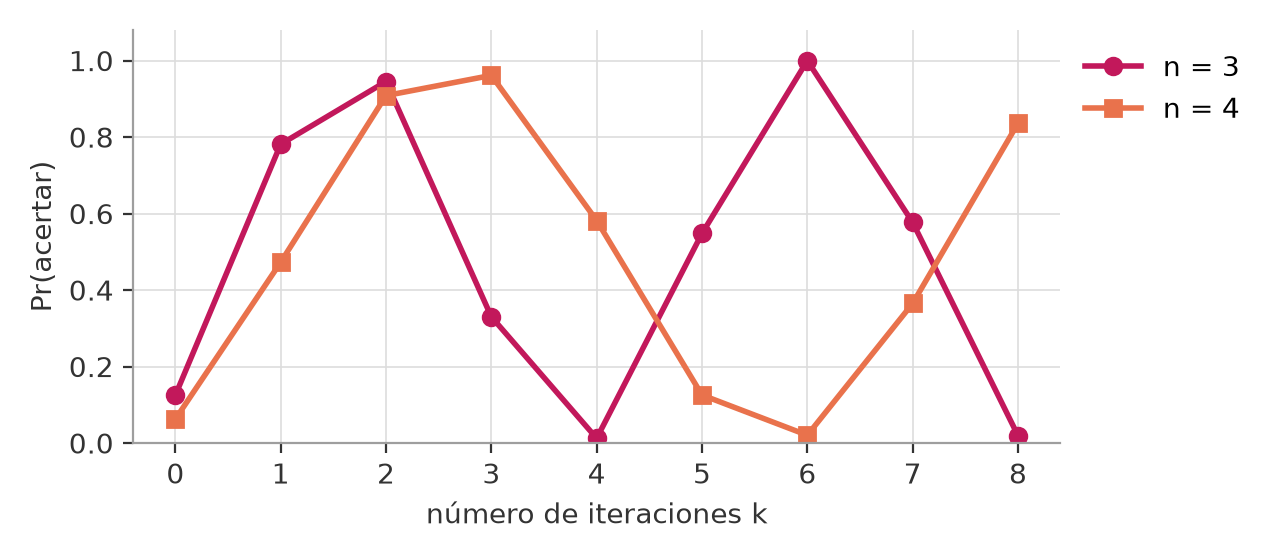
\includegraphics[width=0.8\textwidth]{grover_probabilidad.png}

\small Probabilidad de acertar frente al número de iteraciones. Es periódica: el estado gira en el plano $\{\ket{\alpha},\ket{\beta}\}$. Los máximos están en $k = 2$ para $n = 3$ y en $k = 3$ para $n = 4$.
\end{cajafigura}

\noindent Las amplitudes del registro tras $k = 1$ y $k = 2$, multiplicadas por $\sqrt8$, son
\begin{codigo}[language={}]
k=1: [-0.5  -0.5  -0.5  -0.5  -0.5  -2.5  -0.5  -0.5 ]
k=2: [-0.25 -0.25 -0.25 -0.25 -0.25  2.75 -0.25 -0.25]
\end{codigo}
\noindent que son las del Ejemplo 6.4.2 ($\frac{1}{2\sqrt8}, \frac{5}{2\sqrt8}$ y $-\frac{1}{4\sqrt8}, \frac{11}{4\sqrt8}$) multiplicadas por $(-1)^k$: cada difusión aporta el signo global $-1$ del Experimento 6.

\noindent Finalmente, con $1000$ disparos:
\begin{codigo}[language={}]
2 iteraciones: {'101': 932, '110': 11, '011': 7, '100': 9, '000': 15, '111': 8, '010': 8, '001': 10}
3 iteraciones: {'011': 102, '100': 99, '101': 346, '001': 91, '110': 81, '000': 86, '010': 93, '111': 102}
\end{codigo}

\begin{cajafigura}
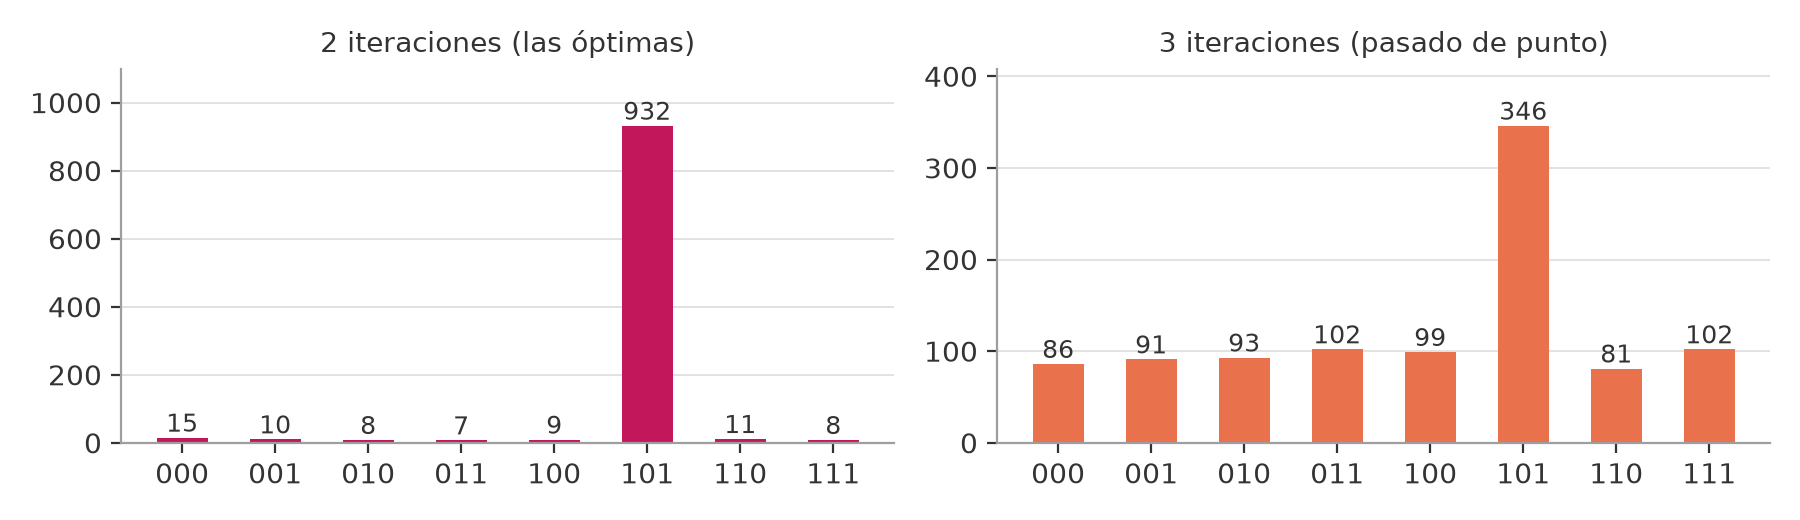
\includegraphics[width=\textwidth]{grover_histogramas.png}

\small Con las $2$ iteraciones óptimas, $\texttt{101}$ sale el $93{,}2\%$ de las veces (teórico: $94{,}5\%$). Con $3$, como sugiere el redondeo de $\sqrt8$, solo el $34{,}6\%$ (teórico: $33{,}0\%$).
\end{cajafigura}

\cleardoublepage
\section{Resumen: un ejemplo guiado}

\noindent Seguimos el ejemplo del libro: $n = 3$, $N = 8$ y el elemento marcado es $\bx_0 = \texttt{101}$.

\pasoguiado{Paso 1. El problema}
{$f(\texttt{101}) = 1$ y $f(\bx) = 0$ para las otras siete cadenas. Hay que encontrar $\texttt{101}$.}
{\textbf{Búsqueda no estructurada.} Clásicamente, $N-1 = 7$ consultas en el peor caso y unas $N/2$ en media.}

\pasoguiado{Paso 2. Superposición uniforme}
{$\ket{s} = \tfrac{1}{\sqrt8}(1,1,1,1,1,1,1,1)$, \quad $\Pr(\texttt{101}) = \tfrac18$.}
{$\ket{s} = H^{\otimes n}\ket{\bcero} = \cos\theta\ket{\alpha} + \sin\theta\ket{\beta}$, con $\sin\theta = \frac{1}{\sqrt N}$.}

\pasoguiado{Paso 3. Inversión de fase}
{$\tfrac{1}{\sqrt8}(1,1,1,1,1,-1,1,1)$: con el auxiliar en $\ket{-}$, el oráculo cambia el signo de $\texttt{101}$.}
{$Z_f = I - 2\ket{\bx_0}\bra{\bx_0}$ (retroceso de fase): \textbf{reflexión} respecto de $\ket{\alpha}$. El auxiliar se prepara en $\ket{-}$ una sola vez.}

\pasoguiado{Paso 4. Inversión respecto de la media}
{Media $\frac{3}{4\sqrt8}$; \quad nuevas amplitudes $\frac{1}{2\sqrt8}$ (siete veces) y $\frac{5}{2\sqrt8}$; \quad $\Pr(\texttt{101}) = \frac{25}{32}\approx0{,}78$.}
{$D = -I+2A = 2\ket{s}\bra{s} - I$: \textbf{reflexión} respecto de $\ket{s}$; unitaria porque $A^2 = A$. Se implementa como $H^{\otimes n}(2\ket{\bcero}\bra{\bcero}-I)H^{\otimes n}$.}

\pasoguiado{Paso 5. Dos reflexiones, un giro}
{$G|_P = \begin{pmatrix}\cos2\theta & -\sin2\theta\\ \sin2\theta & \cos2\theta\end{pmatrix}$, \quad $\theta\approx20{,}7^\circ$: cada iteración gira $41{,}4^\circ$ hacia $\ket{\texttt{101}}$.}
{\textbf{Teorema:} $G^k\ket{s}$ forma un ángulo $(2k+1)\theta$ con $\ket{\alpha}$, y $\Pr(\bx_0) = \sin^2((2k+1)\theta)$.}

\pasoguiado{Paso 6. Segunda iteración}
{Amplitudes $-\frac{1}{4\sqrt8}$ (siete veces) y $\frac{11}{4\sqrt8}\approx0{,}972$; \quad $\Pr(\texttt{101}) = \frac{121}{128}\approx0{,}945 = \sin^2(5\theta)$.}
{$k = \lfloor\pi/(4\theta)\rfloor = 2$ iteraciones: $\Pr\ge1-\frac1N$.}

\pasoguiado{Paso 7. No pasarse}
{Con $k = 3$: $\Pr = 0{,}330$. Qiskit, $1000$ disparos: $932$ aciertos con $k = 2$ y $346$ con $k = 3$.}
{El número de iteraciones es $\approx\frac{\pi}{4}\sqrt N$, \textbf{no} $\sqrt N$: el giro continúa y se aleja de la solución. Ventaja \textbf{cuadrática}, que es óptima.}

\begin{center}
\small\renewcommand{\arraystretch}{1.15}
\begin{tabular}{c|l|l}
\textbf{Paso} & \textbf{Qué hicimos} & \textbf{Concepto} \\ \hline
1 & Buscar $\texttt{101}$ & Búsqueda no estructurada; cota clásica $\sim N$ \\
2 & $H^{\otimes3}\ket{000}$ & Estado uniforme, ángulo $\theta$ \\
3 & Cambiar un signo & Inversión de fase = reflexión \\
4 & $v\mapsto2a - v$ & Inversión respecto de la media = reflexión \\
5 & $G = DZ_f$ & Dos reflexiones = giro de $2\theta$ \\
6 & Segunda iteración & $\sin^2(5\theta) = \frac{121}{128}$ \\
7 & Tercera iteración & Pasarse de cocción; $k\approx\frac{\pi}{4}\sqrt N$
\end{tabular}
\end{center}

% ========================= BIBLIOGRAFÍA =============================
\cleardoublepage
\begin{thebibliography}{99}

\bibitem{yanofsky2008}
N.~S.~Yanofsky y M.~A.~Mannucci.
\newblock \emph{Quantum Computing for Computer Scientists}.
\newblock Cambridge University Press, 2008. Capítulo 6, secciones 6.1--6.4.

\bibitem{deutsch1985}
D.~Deutsch.
\newblock Quantum theory, the Church--Turing principle and the universal quantum computer.
\newblock \emph{Proceedings of the Royal Society of London A}, 400:97--117, 1985.

\bibitem{deutsch1992}
D.~Deutsch y R.~Jozsa.
\newblock Rapid solution of problems by quantum computation.
\newblock \emph{Proceedings of the Royal Society of London A}, 439:553--558, 1992.

\bibitem{cleve1998}
R.~Cleve, A.~Ekert, C.~Macchiavello y M.~Mosca.
\newblock Quantum algorithms revisited.
\newblock \emph{Proceedings of the Royal Society of London A}, 454:339--354, 1998.

\bibitem{simon1997}
D.~R.~Simon.
\newblock On the power of quantum computation.
\newblock \emph{SIAM Journal on Computing}, 26(5):1474--1483, 1997. (Versión de congreso: FOCS 1994.)

\bibitem{grover1996}
L.~K.~Grover.
\newblock A fast quantum mechanical algorithm for database search.
\newblock En \emph{Proceedings of the 28th Annual ACM Symposium on Theory of Computing (STOC)}, 212--219, 1996.

\bibitem{boyer1998}
M.~Boyer, G.~Brassard, P.~Høyer y A.~Tapp.
\newblock Tight bounds on quantum searching.
\newblock \emph{Fortschritte der Physik}, 46:493--505, 1998.

\bibitem{bennett1997}
C.~H.~Bennett, E.~Bernstein, G.~Brassard y U.~Vazirani.
\newblock Strengths and weaknesses of quantum computing.
\newblock \emph{SIAM Journal on Computing}, 26(5):1510--1523, 1997.

\bibitem{nielsen2010}
M.~A.~Nielsen e I.~L.~Chuang.
\newblock \emph{Quantum Computation and Quantum Information}.
\newblock Cambridge University Press, edición del 10.º aniversario, 2010.

\bibitem{watrous2024understanding}
J.~Watrous.
\newblock \emph{Understanding Quantum Information and Computation}.
\newblock IBM Quantum Learning.
\newblock \url{https://quantum.cloud.ibm.com/learning}

\bibitem{havlicek2019supervised}
V.~Havlíček, A.~D.~Córcoles, K.~Temme, A.~W.~Harrow, A.~Kandala, J.~M.~Chow y J.~M.~Gambetta.
\newblock Supervised learning with quantum-enhanced feature spaces.
\newblock \emph{Nature}, 567:209--212, 2019.

\bibitem{thanasilp2024exponential}
S.~Thanasilp, S.~Wang, M.~Cerezo y Z.~Holmes.
\newblock Exponential concentration in quantum kernel methods.
\newblock \emph{Nature Communications}, 15:5200, 2024.

\end{thebibliography}

\end{document}
